\documentclass[12pt]{article}

\usepackage[margin=1in,footskip=0.25in]{geometry}
\usepackage[hyphens]{url}
\usepackage{graphicx}% demo option just for the example
\usepackage{caption}
\usepackage{color}
\usepackage{hyperref}
\usepackage{textcomp}
\usepackage{fancyhdr}
\pagestyle{fancy}
% http://tex.stackexchange.com/questions/20890/define-an-escape-underscore-environment
\usepackage[T1]{fontenc}
\catcode`\_=12


\lhead{OpenWarp Configuration and Deployment Guide}
%\rhead{this is page \thepage}
\cfoot{Topcoder \textcopyright{} 2016}
\renewcommand{\headrulewidth}{0.4pt}
\renewcommand{\footrulewidth}{0.4pt}

%opening
\title{Deployment Guide}
\author{yedtoss}

\newcommand{\ROOT}{{\textbf{\$ROOT}}}
\newcommand{\NEMOHFORTRAN}{{\textbf{\$NEMOH{\_}FORTRAN}}}
\newcommand{\NEMOHPYTHON}{{\textbf{\$NEMOH{\_}PYTHON}}}
\newcommand{\FORTRANBUILD}{{\textbf{\$FORTRAN{\_}BUILD}}}
\newcommand{\MINGWROOT}{{\textbf{\$MINGW{\_}ROOT}}}
\newcommand{\INSTALLDIR}{{\textbf{\$INSTALL{\_}DIR}}}



\begin{document}\sloppy

\maketitle
\thispagestyle{empty}
\tableofcontents
\newpage

\section{INTRODUCTION}
OpenWarp is a web application that can mesh and simulate a body of an offshore structure.
It computes the first-order forces (added mass, radiation damping, and diffraction forces) on the body and solves the radiation-diffraction problem of first order.

The OpenWarp software package is composed of three main parts. The first part is the meshing tool. The tool can take as input a raw body in STEP, STL, or IGS format and generate its corresponding shell.
The second part of OpenWarp, called Nemoh Solver, is an application that solves the problem of seakeeping in hydrodynamics. It uses the boundary element method to solve for bodies partially immersed (floating) or completely immersed in a fluid of infinite or constant finite depth, with or without forward speed subject to sinusoidal waves. It can be used with the first-order or higher-order panel method.
The third part postprocesses the results obtained by Nemoh Solver and generates TECPLOT files of diffraction, radiation, and excitation forces. Added mass and damping coefficients are also generated in TECPLOT format.

OpenWarp operates on an input mesh. To get the input mesh in the correct format, one should use the meshing tool, which can generate a thin or non-thin mesh from an existing body described in STEP, STL, or IGS format. To solve the radiation and diffraction problem, we must represent the body with multiple (thin) quadrilateral elements or shells.
OpenWarp includes a web application which can be used to mesh, simulate, and postprocess a body. This web application has a graphical interface that is powered by a server which the user runs locally.

OpenWarp has been developed by the Department of Energy and Topcoder. It is expected to be used by people developing Wave Energy Conversion (WEC) devices in the United States. Until now the testing of new WEC devices has been expensive and time-consuming. OpenWarp will spur innovation by enabling wave-energy startups to develop, analyze, and optimize their devices more quickly.

\section{OVERVIEW}
Immediately below, we list the notations used in this document and describe the software dependencies for OpenWarp deployment. In subsequent sections, we give detailed instructions for deploying OpenWarp on Windows and on OS X. Finally, we describe how to configure OpenWarp and give a practical usage example

\section{NOTATIONS}

The following notations are used in this document.
\begin{description}
	\item[\ROOT{}] : the top-level directory of the Nemoh software package.
	\item[\NEMOHFORTRAN]: the directory \ROOT{}/NemohImproved/Nemoh/ 
	\item[\FORTRANBUILD{}]: the build directory for the FORTRAN version of Nemoh.
	\item[\MINGWROOT]: the directory where MinGW will be installed.
	\item [\INSTALLDIR] is used in the following to mean the root directory containing the files you get when you install the currently available installer for each os.
	\item [\NEMOHPYTHON]: the directory \ROOT{}/openwarpgui/nemoh
\end{description}


\section{DEPENDENCIES}
OpenWarp is compatible with Windows and OS X.
Below are the software packages needed to install the application. Section 5 provides step-by-step instructions for Windows installation and section 6 does likewise for OS X.

\subsection{Windows}

\begin{itemize}
\item \textbf{Windows 7/8 64 bits} (Other versions might work but not tested)
\item MinGW $4.8.1$ \url{http://sourceforge.net/projects/MinGWbuilds/files/host-windows/releases/4.8.1/}
\item BLAS \url{http://icl.cs.utk.edu/lapack-for-windows/lapack/\#libraries} 
\item LAPACK  \url{http://icl.cs.utk.edu/lapack-for-windows/lapack/\#libraries} 
\item OpenMP provided by MinGW
\item HDF5 $>=1.8.11$  \url{http://www.hdfgroup.org/HDF5/}  Optionally provided by Anaconda
\item HDFView \url{http://www.hdfgroup.org/products/java/release/download.html}
Python 2.7 Optionally provided by Anaconda
\item H5py $>= 2.3.1$ Optionally provided by Anaconda
\item NumPy Optionally provided by Anaconda
\item CMake $>= 2.8$ \url{http://www.cmake.org/cmake/resources/software.html}
\item Anaconda (with Python 2.7) $>= 2.1.0$ \url{http://continuum.io/downloads} 
\item ParaView $>=4.1$  \url{http://www.paraview.org/download/}
\end{itemize}



\subsection{OS X}
\label{mac-deps}
\begin{itemize}
\item \textbf{MAC OS X 10.10 64 bits} (Other versions might work but not tested)
\item Homebrew (brew command) \url{http://brew.sh/}
\item GCC $>= 4.8$ installed by brew
\item Xcode Command Line Tools installed by brew
\item BLAS provided by XCode commands 
\item LAPACK  Provided by XCode commands
\item OpenMP provided by GCC
\item HDF5 $>=1.8.11$  \url{http://www.hdfgroup.org/HDF5/} Optionally provided by Anaconda
\item HDFView \url{http://www.hdfgroup.org/products/java/release/download.html}
\item Python $2.7$ Optionally provided by Anaconda
\item H5py $>= 2.3.1$ Optionally provided by Anaconda
\item NumPy Optionally provided by Anaconda
\item CMake $>= 2.8$ installed by brew 
\item Anaconda (with Python$ 2.7$) $>= 2.1.0$ \url{http://continuum.io/downloads} 
\item ParaView $>=4.1$  \url{http://www.paraview.org/download/}

\end{itemize}

\subsection{Linux}

\begin{itemize}
	\item Linux/Ubuntu 14.04 64 bits (Other versions might work but not tested)
	\item Except from Homebrew and XCode, Linux shared the same dependencies as MAC OSX as listed in section \ref{mac-deps}.
\end{itemize}

\section{Building from scratch}

\subsection{WINDOWS DEPLOYMENT FROM SCRATCH}
\label{ws}

Only 64-bit versions of Windows 7 and Windows 8 are supported.
To deploy the application on Windows, perform the following steps:

\begin{itemize}
	\item Download MinGW (64-bit) from \url{http://sourceforge.net/projects/mingwbuilds/files/host-windows/releases/4.8.1/64-bit/threads-posix/sjlj/x64-4.8.1-release-posix-sjlj-rev5.7z/download}.
	
	\item Extract it to a directory, making sure that the directory name contains no spaces. Let's denote this directory as \MINGWROOT.
	
	\item Add \MINGWROOT{}\textbackslash{}bin and \MINGWROOT{}\textbackslash{}lib to the beginning of your Windows PATH by opening the System control panel and editing Properties $\rightarrow$ Advanced System Settings  $\rightarrow$ Advanced tab  $\rightarrow$ Environment Variables  $\rightarrow$ Path as shown in this screenshot:
	
	\vspace{\abovedisplayskip}
	\begin{minipage}{\linewidth}
		\centering
		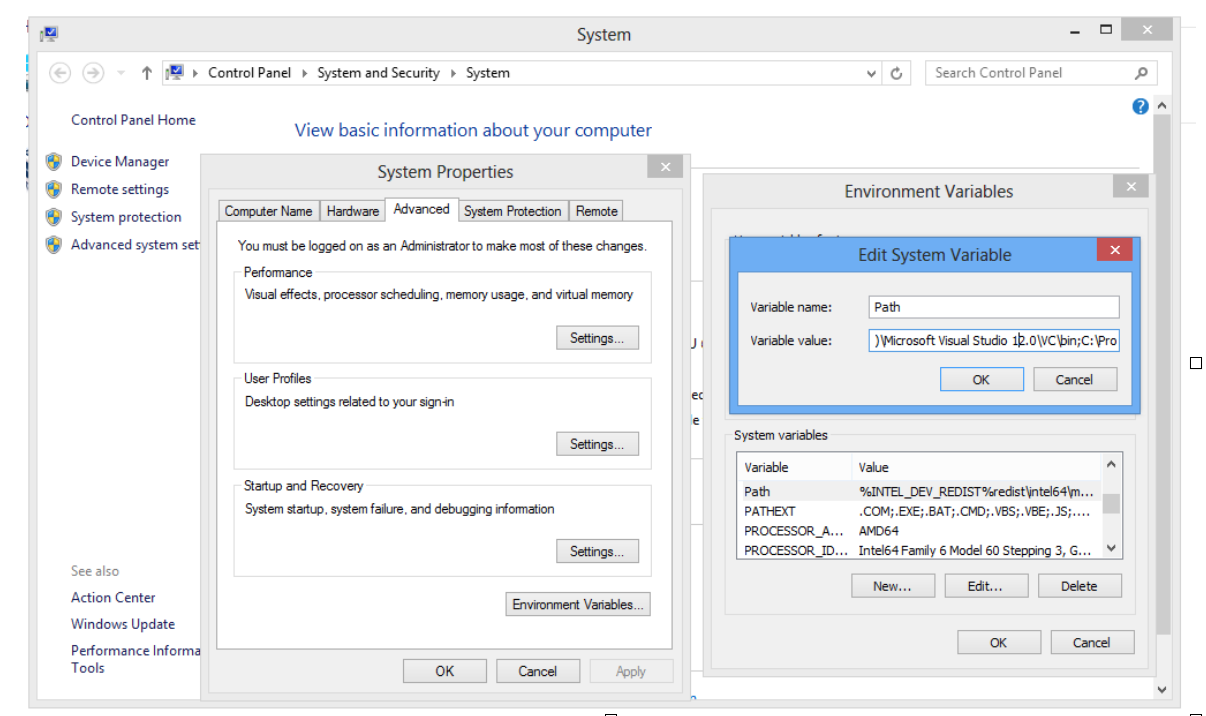
\includegraphics[scale=0.75]{img/1}
		%\captionof{figure}{Transfer from R1 to R2 whenK1=1}
	\end{minipage}
	\vspace{\belowdisplayskip}
	
	\item Copy \ROOT{}/src/bundled/simulation/libs/libnemoh.dll,  \ROOT{}/src/bundled/simulation/libs/libnemoh.dll.a, \\
	 \ROOT{}/src/bundled/simulation/libs/libblas.dll, and
	  \ROOT{}/src/bundled/simulation/libs/liblapack.dll to \MINGWROOT{}/lib.
	
	
	\item Download and install Anaconda 2.10 with Python 2.7 for Windows (64-bit, graphical installer) from \url{http://continuum.io/downloads}.
	If you install it to C:/Users/bob/Anaconda for example, make sure that you manually add C:/Users/bob/Anaconda and C:/Users/bob/Anaconda/Scripts to the beginning of your Windows PATH variable. Don't forget to replace bob with your own user name.
	
	
	\item Once the preceding steps are done, start PowerShell and install the CherryPy dependencies by executing this command in the \ROOT{}/src/ directory:
{\color{blue}pip install -r requirements.txt}

\vspace{\abovedisplayskip}
\begin{minipage}{\linewidth}
	\centering
	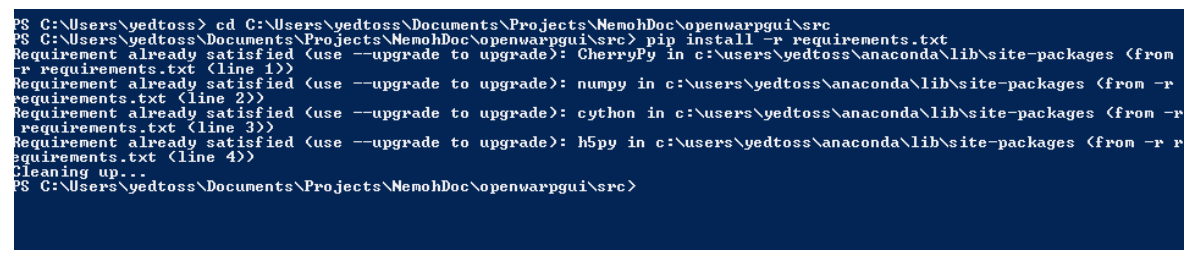
\includegraphics[scale=0.75]{img/2}
	%\captionof{figure}{Transfer from R1 to R2 whenK1=1}
\end{minipage}
\vspace{\belowdisplayskip}

 \item Start the server by executing this in the src/ directory:
 \textcolor{blue}{python main.py}
 
 \vspace{\abovedisplayskip}
 \begin{minipage}{\linewidth}
 	\centering
 	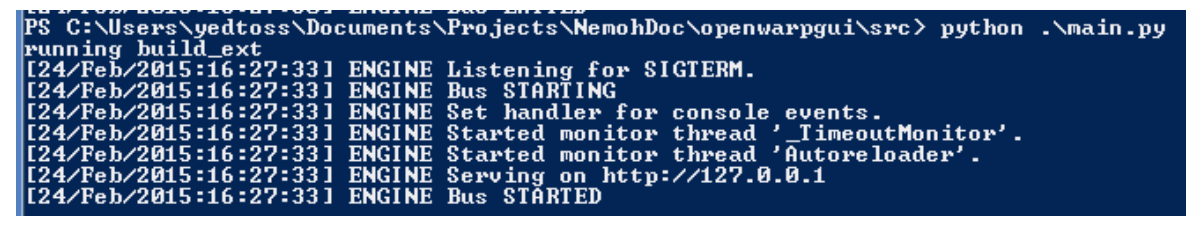
\includegraphics[scale=0.75]{img/3}
 	%\captionof{figure}{Transfer from R1 to R2 whenK1=1}
 \end{minipage}
 \vspace{\belowdisplayskip}
 
 \item Optionally, download the .zip version of ParaView from \url{http://www.paraview.org/download/}  and copy it to src/bundled/paraview so that src/bundled/paraview/bin exists. This is only needed for testing the visualization of the results in ParaView.
 
 \vspace{\abovedisplayskip}
  \begin{minipage}{\linewidth}
  	\centering
  	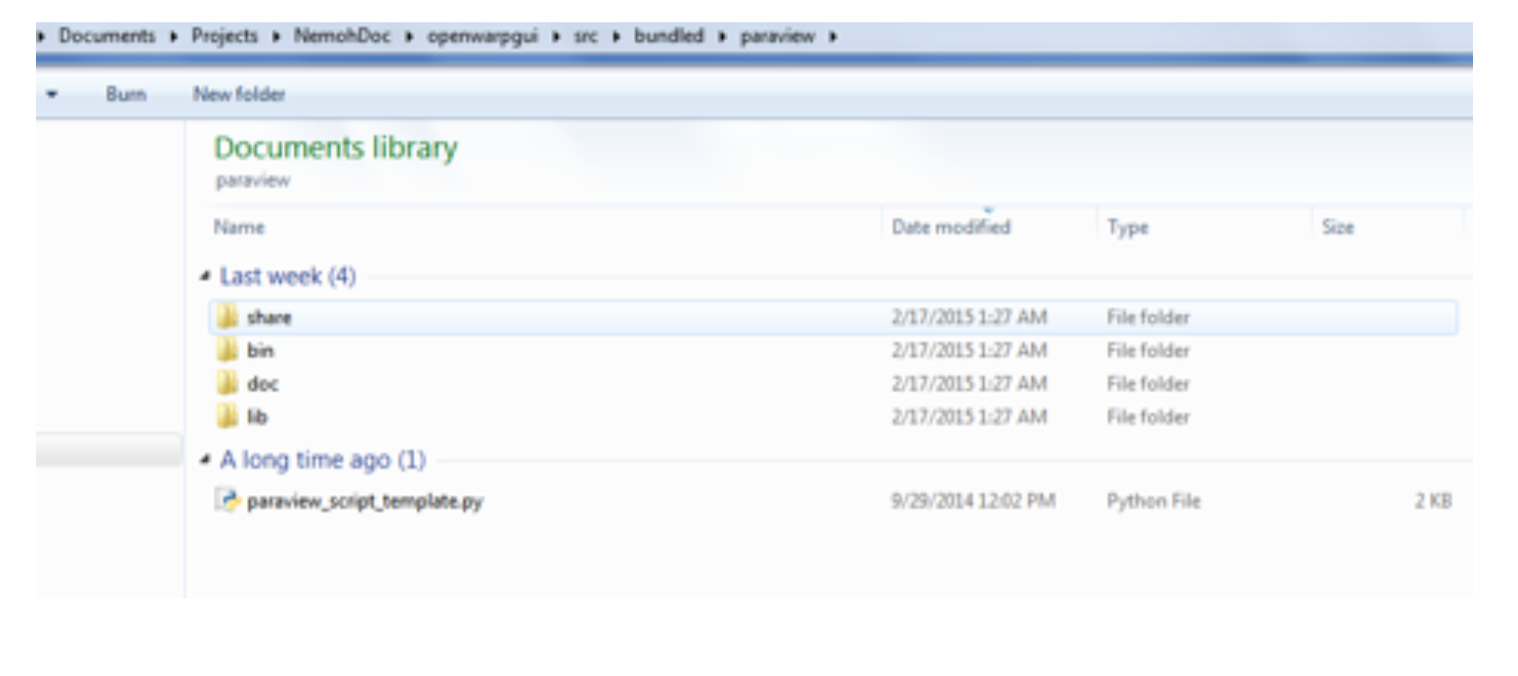
\includegraphics[scale=0.6]{img/4}
  	%\captionof{figure}{Transfer from R1 to R2 whenK1=1}
  \end{minipage}
  \vspace{\belowdisplayskip}
  
  \item If the provided libnemoh.dll and libnemoh.dll.a do not work, you can generate them manually by  doing the following:
  
  \begin{itemize}
  	\item Download CMake from \url{http://www.cmake.org/files/v2.8/cmake-2.8.12.2-win32-x86.exe} , install it and make sure it is in your PATH variable.
  	
  \item 	Start PowerShell and enter an empty directory. Then run:
  	
  	\item  \textcolor{blue}{cmake -DCMAKE{\_}Fortran{\_}COMPILER="gfortran" "\NEMOHFORTRAN{}" -G "MinGW Makefiles"}
  	And  finally run:
  	 \textcolor{blue}{mingw32-make}
  \end{itemize}
 
 
\end{itemize}


\subsection{OS X DEPLOYMENT FROM SCRATCH}
\label{os}
The following instructions are known to work on OS X versions 10.9 and 10.10.
To deploy the application in OS X, perform the following step:

\begin{itemize}
	\item Install brew: {ruby -e \color{blue} "\$(curl -fsSL \url{https://raw.githubusercontent.com/Homebrew/install/master/install})}".
	
	\vspace{\abovedisplayskip}
	\begin{minipage}{\linewidth}
		\centering
		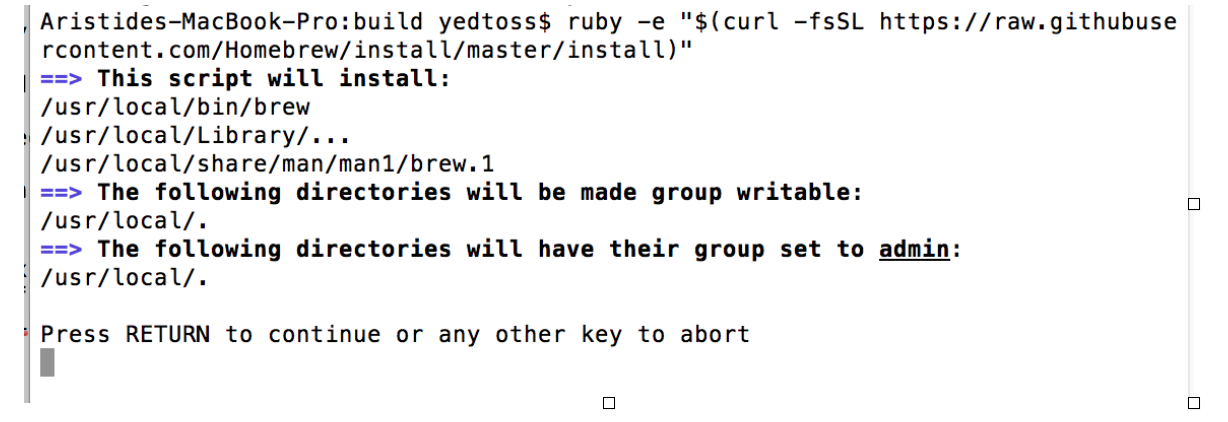
\includegraphics[scale=0.75]{img/5}
		%\captionof{figure}{Transfer from R1 to R2 whenK1=1}
	\end{minipage}
	\vspace{\belowdisplayskip}
	
	\item If you do not have the Xcode command-line tools, you will be prompted to install them as shown below.
	
	\vspace{\abovedisplayskip}
	\begin{minipage}{\linewidth}
		\centering
		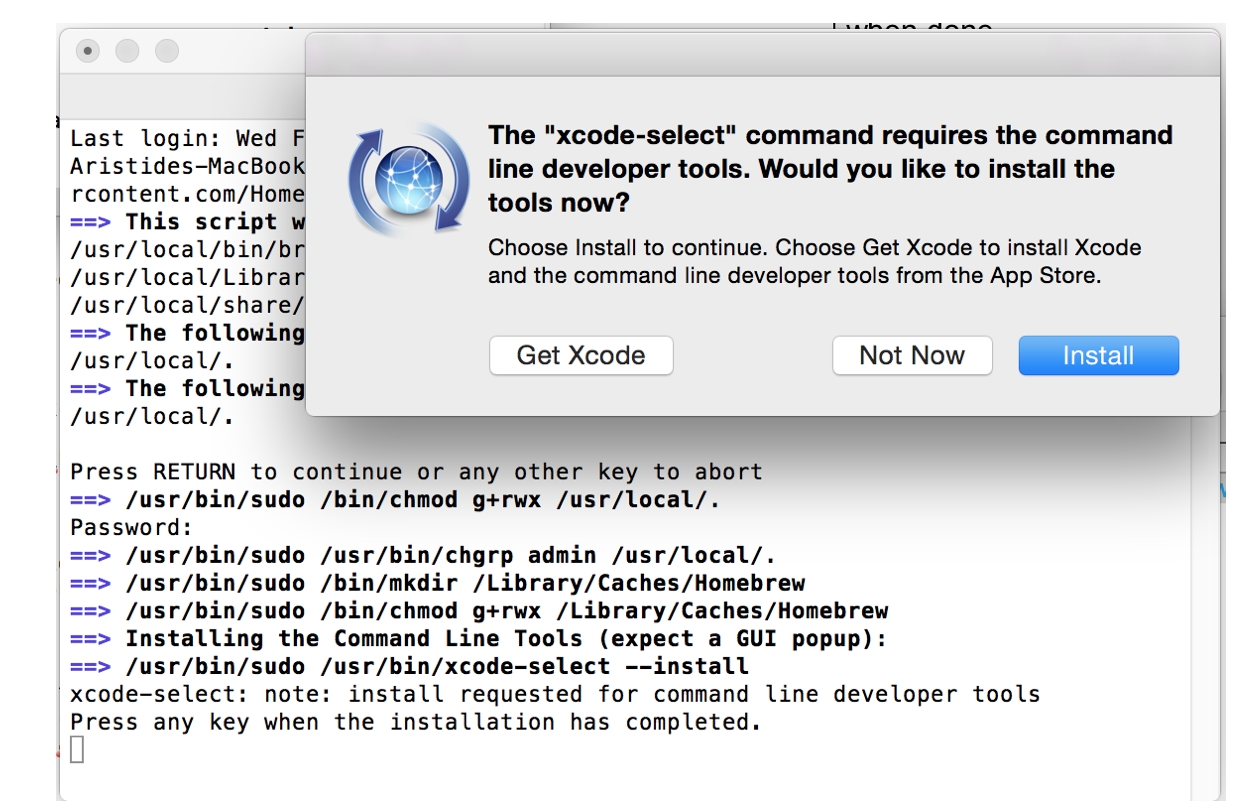
\includegraphics[scale=0.75]{img/6}
		%\captionof{figure}{Transfer from R1 to R2 whenK1=1}
	\end{minipage}
	\vspace{\belowdisplayskip}
	
	\item Install the software and make sure the installation is successful as shown below.
	
	\vspace{\abovedisplayskip}
	\begin{minipage}{\linewidth}
		\centering
		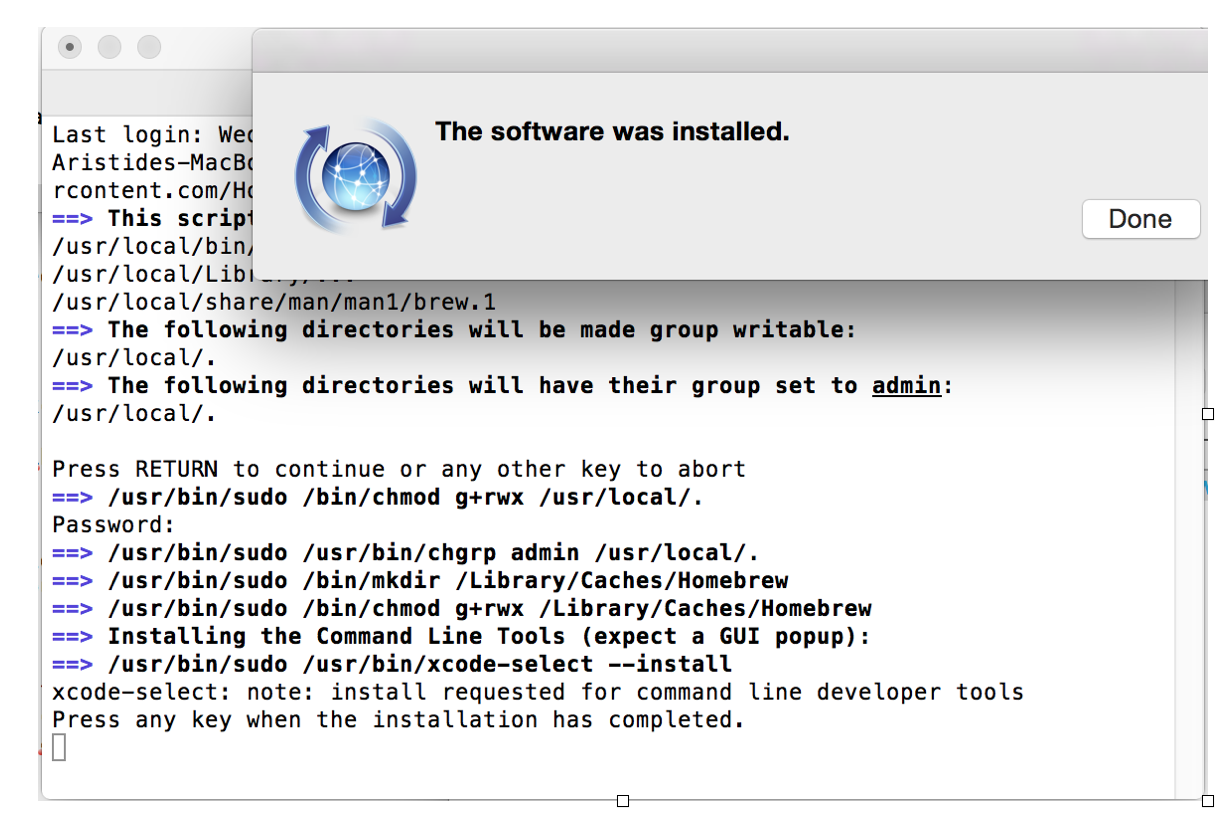
\includegraphics[scale=0.75]{img/7}
		%\captionof{figure}{Transfer from R1 to R2 whenK1=1}
	\end{minipage}
	\vspace{\belowdisplayskip}
	
	\item Press any key. It is possible that you will see an error about the active developer path:
	
	\vspace{\abovedisplayskip}
		\begin{minipage}{\linewidth}
			\centering
			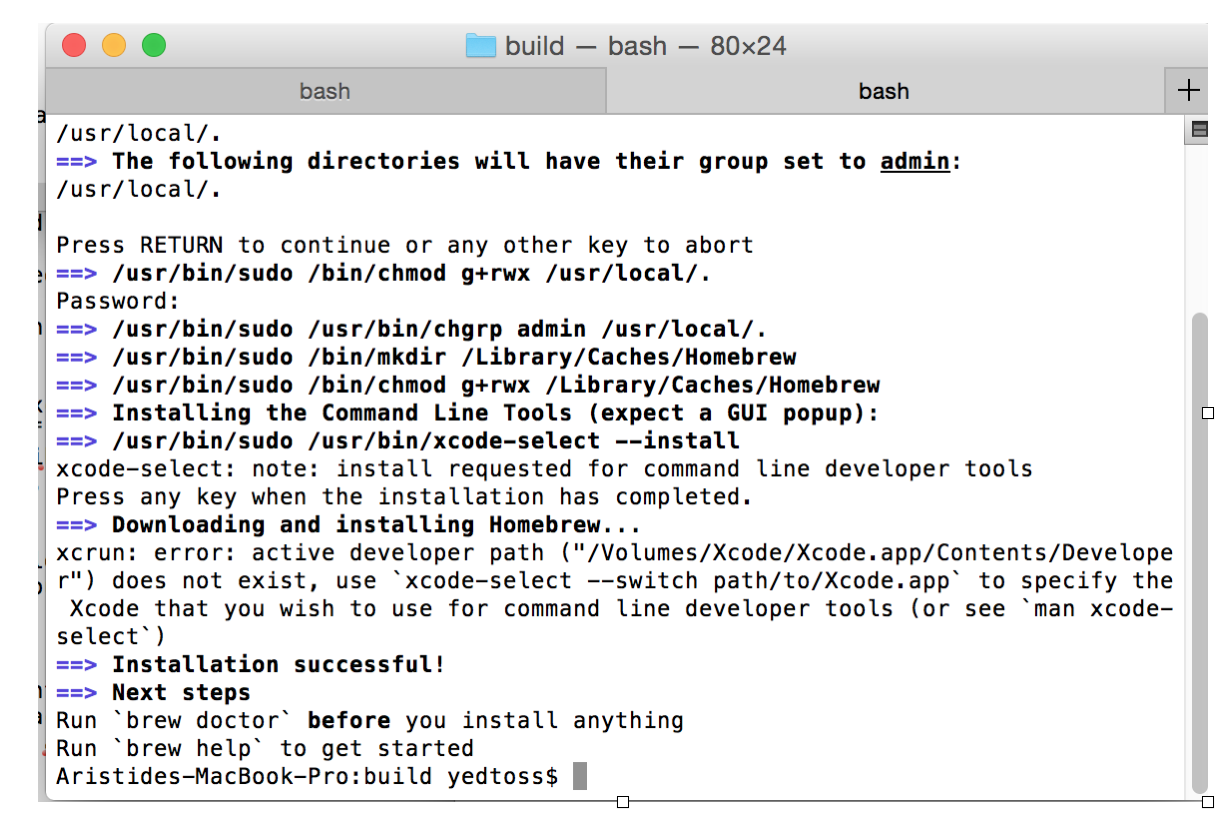
\includegraphics[scale=0.75]{img/8}
			%\captionof{figure}{Transfer from R1 to R2 whenK1=1}
		\end{minipage}
		\vspace{\belowdisplayskip}
		
		\item If you do get that error, you can correct it by specifying the version of Xcode to use:
		{ \color{blue} sudo xcode-select --switch /Applications/Xcode.app}
		
		\vspace{\abovedisplayskip}
		\begin{minipage}{\linewidth}
			\centering
			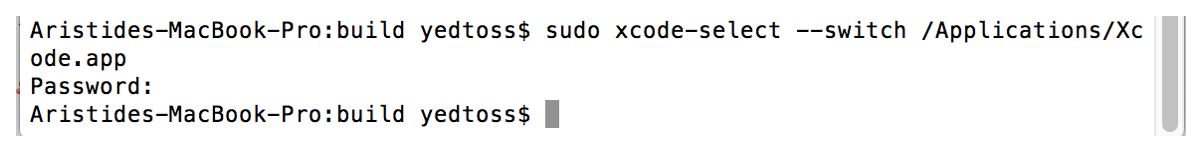
\includegraphics[scale=0.75]{img/9}
			%\captionof{figure}{Transfer from R1 to R2 whenK1=1}
		\end{minipage}
		\vspace{\belowdisplayskip}
		
		\item Now run this command:
			{ \color{blue} brew doctor}
			
			\vspace{\abovedisplayskip}
			\begin{minipage}{\linewidth}
				\centering
				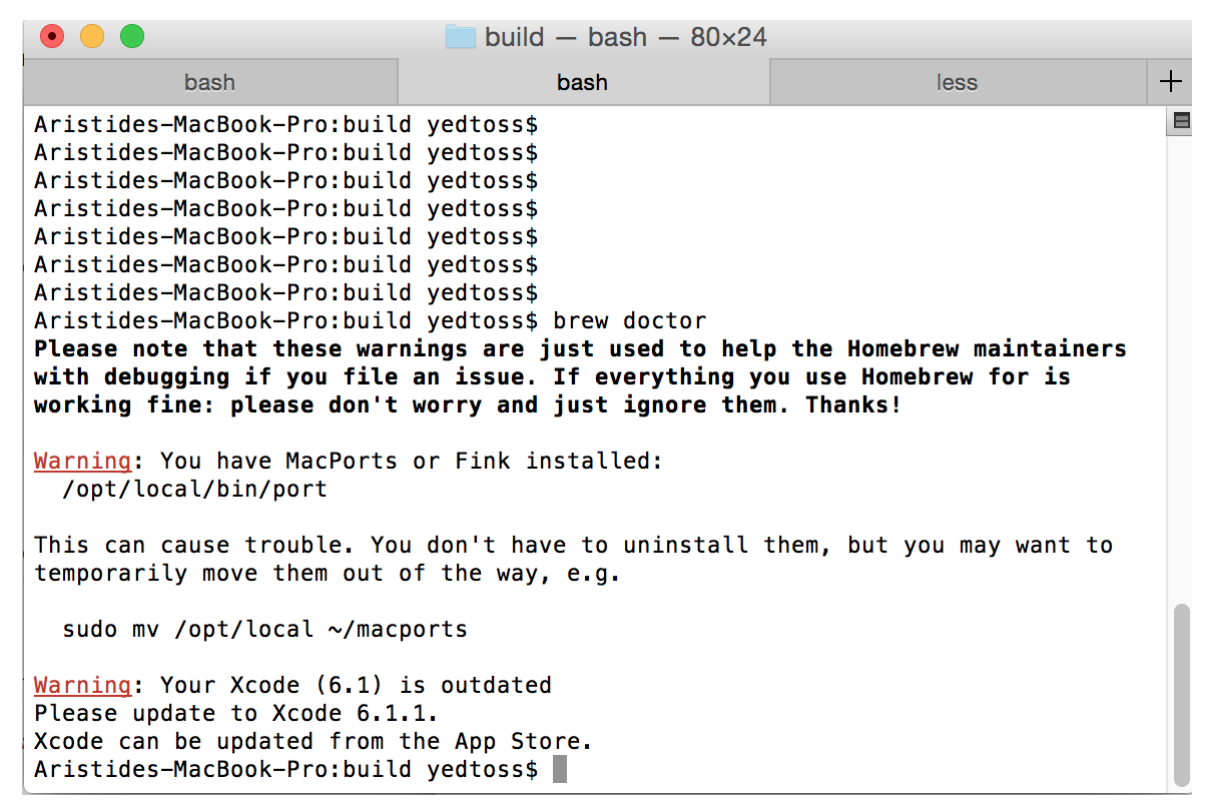
\includegraphics[scale=0.75]{img/10}
				%\captionof{figure}{Transfer from R1 to R2 whenK1=1}
			\end{minipage}
			\vspace{\belowdisplayskip}
			
			\item Ignore any warnings that may appear.
			Install GCC and GFortran:
				{ \color{blue} brew install gcc}
			You can ignore warnings about multilib.
			
				\vspace{\abovedisplayskip}
				\begin{minipage}{\linewidth}
					\centering
					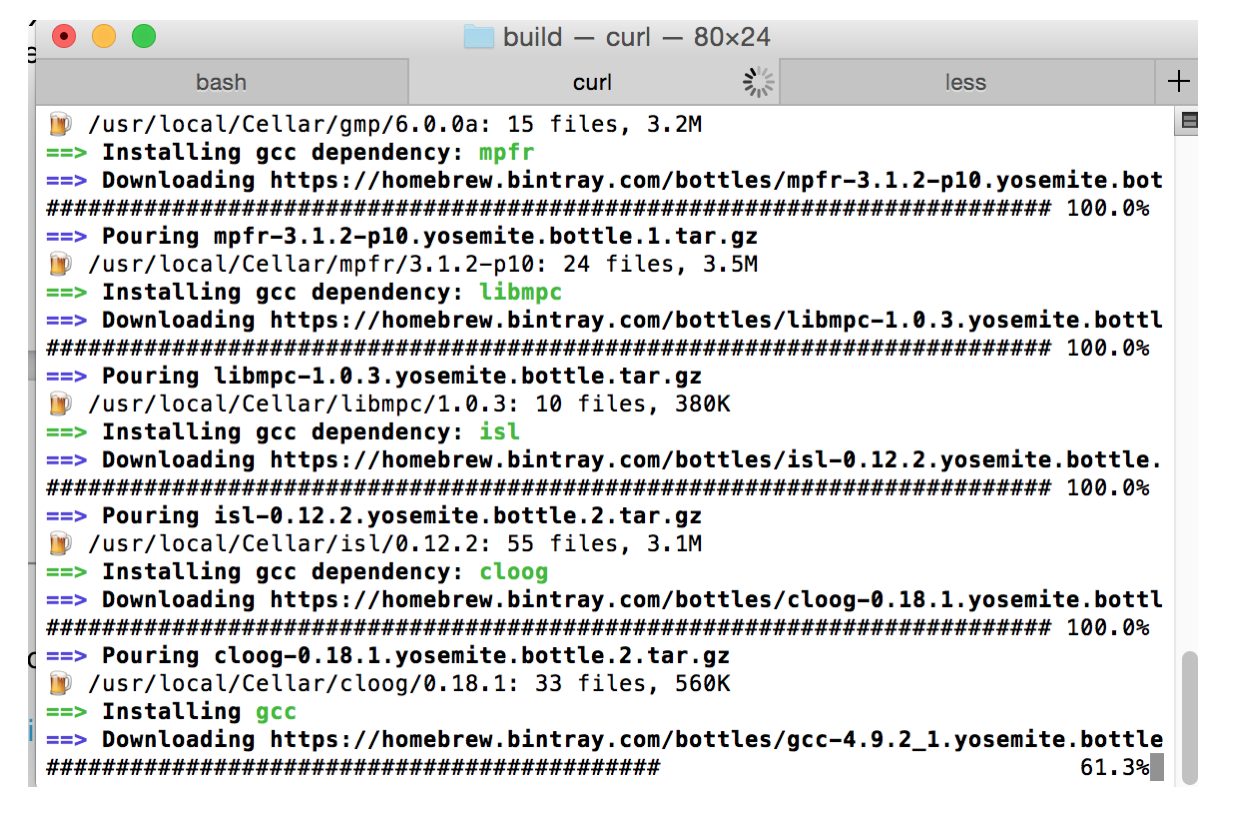
\includegraphics[scale=0.75]{img/11}
					%\captionof{figure}{Transfer from R1 to R2 whenK1=1}
				\end{minipage}
				\vspace{\belowdisplayskip}
				
				\item Install CMake:
					{ \color{blue} brew install cmake}
					
						\vspace{\abovedisplayskip}
						\begin{minipage}{\linewidth}
							\centering
							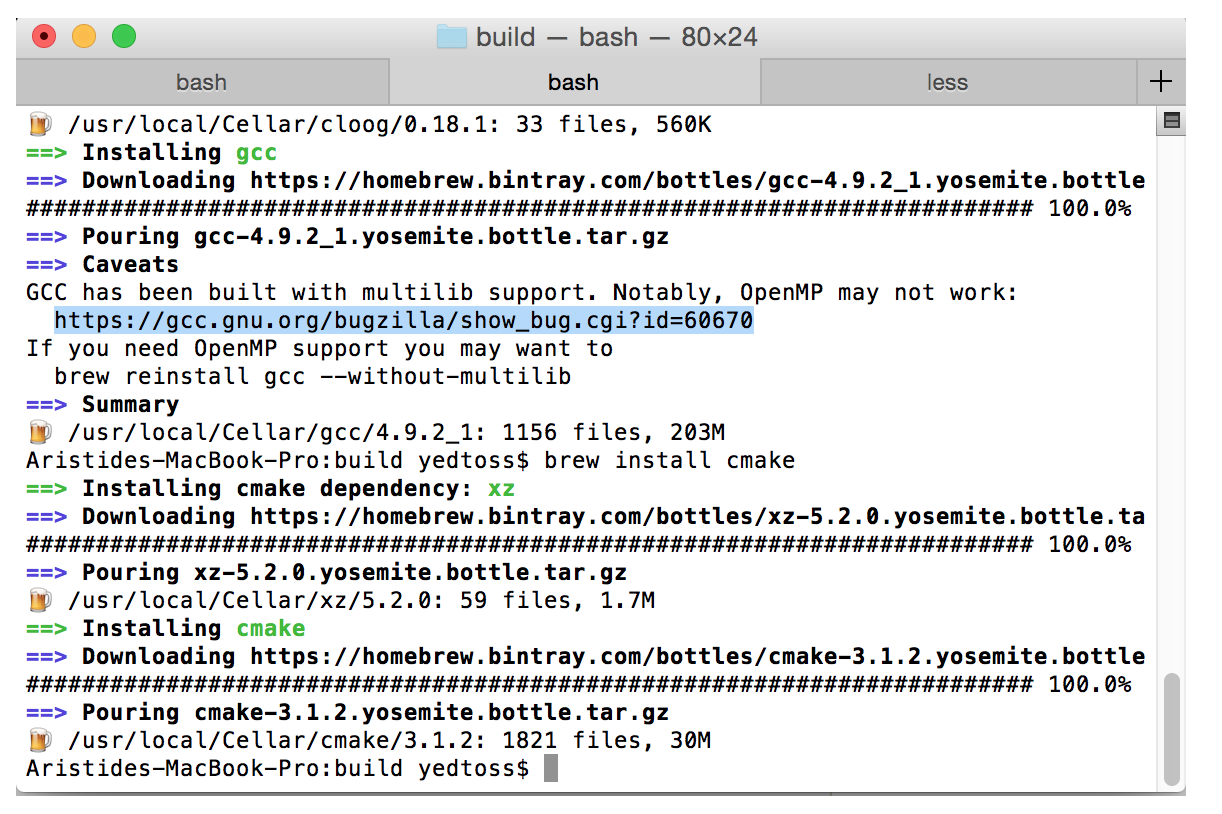
\includegraphics[scale=0.75]{img/12}
							%\captionof{figure}{Transfer from R1 to R2 whenK1=1}
						\end{minipage}
					\vspace{\belowdisplayskip}
					
					\item 
					Download and install Anaconda for OS X, 64-bit version with Python 2.7 and graphical installer, from \url{http://continuum.io/downloads}.  
					
					\vspace{\abovedisplayskip}
						\begin{minipage}{\linewidth}
							\centering
							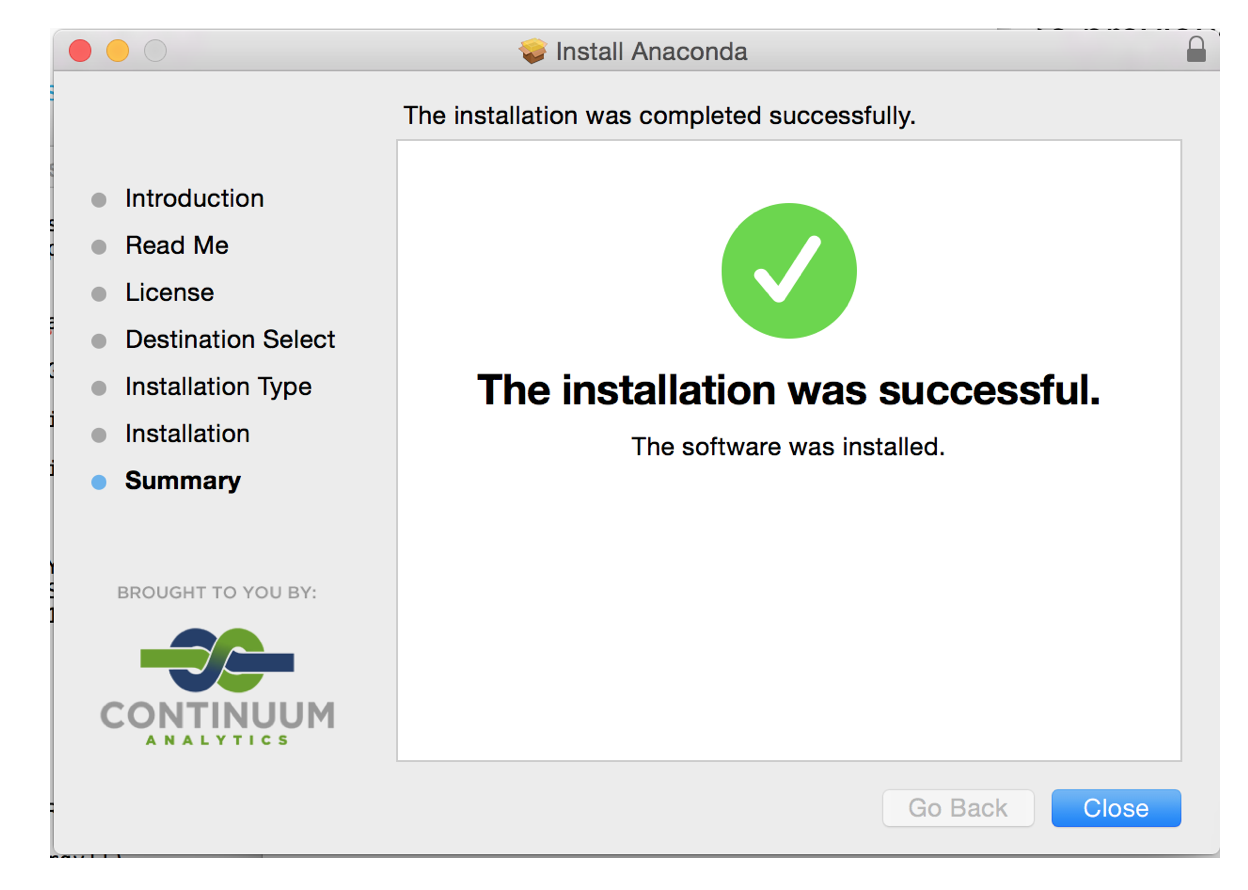
\includegraphics[scale=0.75]{img/13}
							%\captionof{figure}{Transfer from R1 to R2 whenK1=1}
						\end{minipage}
					\vspace{\belowdisplayskip}
					
					\item Now we are going to compile Nemoh Fortran in order to generate the libraries used by the OpenWarp web application. In the following, \NEMOHFORTRAN is the directory NemohMerged/Nemoh/ within the top-level OpenWarp directory.
					\item Create a new directory different from \NEMOHFORTRAN. Let's call this directory \FORTRANBUILD.
					\item Go to \FORTRANBUILD:
					{ \color{blue}cd \FORTRANBUILD}
					
					\item 
					This step is optional for a local testing. However if you want to redistribute or create an installer you MUST do it.
					
					Make sure that the dynamic version of quadmath library is not in your path by running the following command. You may have to adapt 4.9 to the version of gcc installed by brew.
					
					\begin{itemize}
						\item (One line command)
						{ \color{blue} mv /usr/local/lib/gcc/4.9/libquadmath.0.dylib /usr/local/lib/gcc/4.9/disable{\_}libquadmath.0.dylib}
						\item (One line command)
						mv /usr/local/lib/gcc/4.9/libquadmath.dylib /usr/local/lib/gcc/4.9/disable{\_}libquadmath.dylib
					\end{itemize}
					
					
					
					
					\item Run this command to compile Nemoh Fortran:
					{ \color{blue}cmake  -DCMAKE{\_}FortranE{\_}COMPILER="gfortran" \NEMOHFORTRAN}
					If you get a warning about CMake policy, ignore it.
					Generate the Nemoh Fortran library by running:
					make
					This causes libnemoh.dylib to be created.
					
						\vspace{\abovedisplayskip}
						\begin{minipage}{\linewidth}
							\centering
							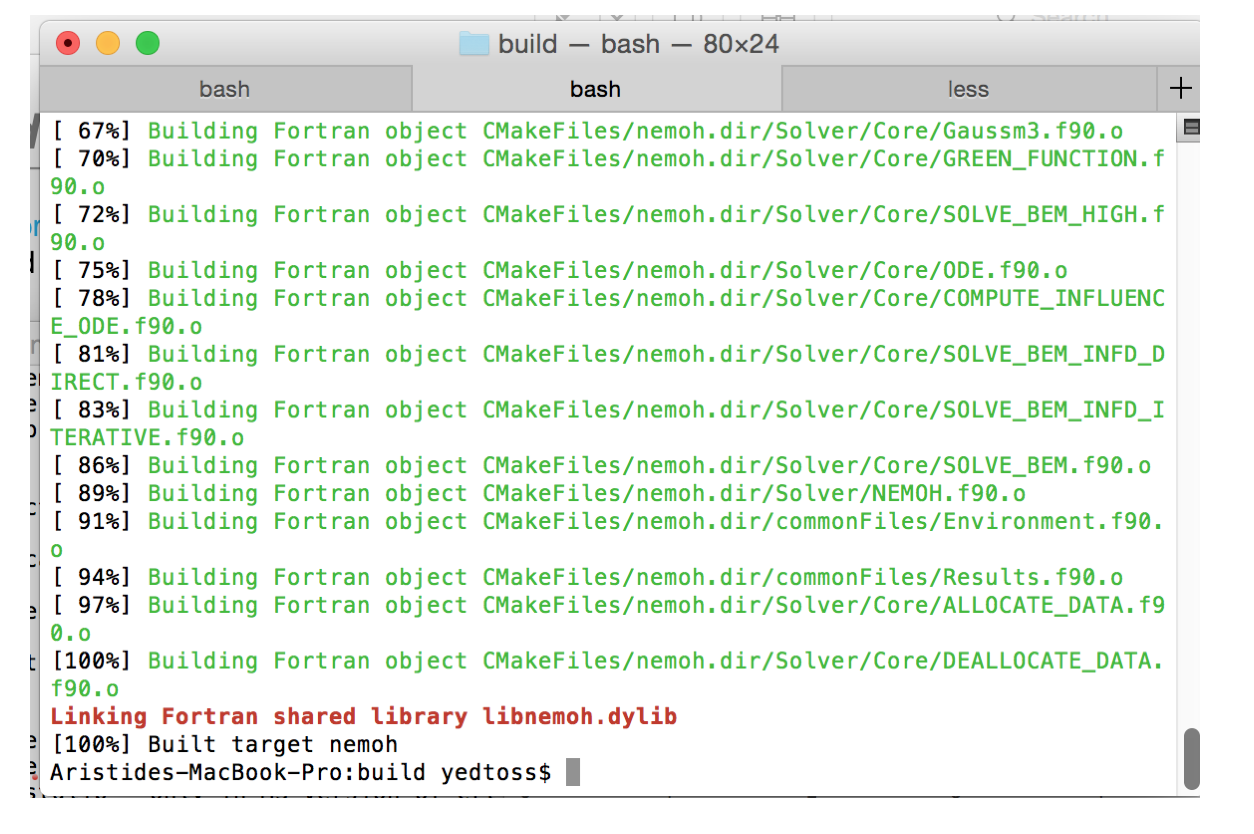
\includegraphics[scale=0.75]{img/14}
							%\captionof{figure}{Transfer from R1 to R2 whenK1=1}
						\end{minipage}
					\vspace{\belowdisplayskip}
					
					
					\item  Copy libnemoh.dylib from \FORTRANBUILD to the lib/ directory inside the Anaconda installation root:
						{ \color{blue}cp \FORTRANBUILD/libnemoh.dylib  /Users/bob/anaconda/lib}
					(Replace "bob" with your own user name.)
					
					
					\item Download the binary installer of ParaView version $>=4.1$ for OS X from \url{http://www.paraview.org/download/}  and install it.
					Next, copy the paraview.app/ folder from the ParaView directory to \ROOT/src/bundled/ so that we can invoke ParaView to do visualization.  (You may need to use sudo if you are performing the copy operation on the command line.) The files under \ROOT/src/bundled/paraview.app/ should be organized as below:
					
					\vspace{\abovedisplayskip}
					\begin{minipage}{\linewidth}
						\centering
						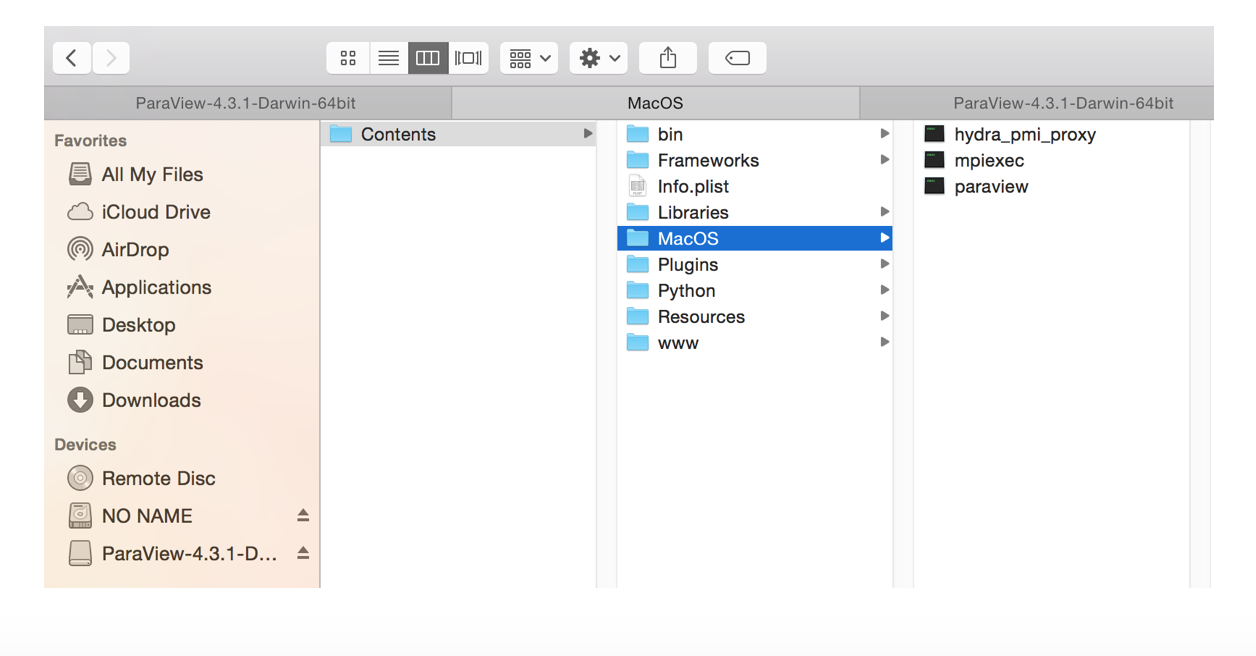
\includegraphics[scale=0.75]{img/15}
						%\captionof{figure}{Transfer from R1 to R2 whenK1=1}
					\end{minipage}
					\vspace{\belowdisplayskip}
					
					
					\item We have to start the OpenWarp server before using the web application. To start the server:
					Make sure you are using Anaconda's version of Python by running:
					{\color{blue} export PATH=/Users/bob/anaconda/bin:\$PATH}
					(Replace "bob" with your own user name.)
					Now run:
					{\color{blue} python \texttt{--}version}
					You should see Anaconda in the output as shown here:
					
					\item Run the following command to verify that the library path is correctly set up:
				
						{\color{blue}(test -e /Users/bob/anaconda/lib/libnemoh.dylib \&\& echo 'Success' ) \texttt{||} echo 'Error: Nemoh library not found'}.
						(As before, replace "bob" with your own user name.)
						
						\vspace{\abovedisplayskip}
						\begin{minipage}{\linewidth}
							\centering
							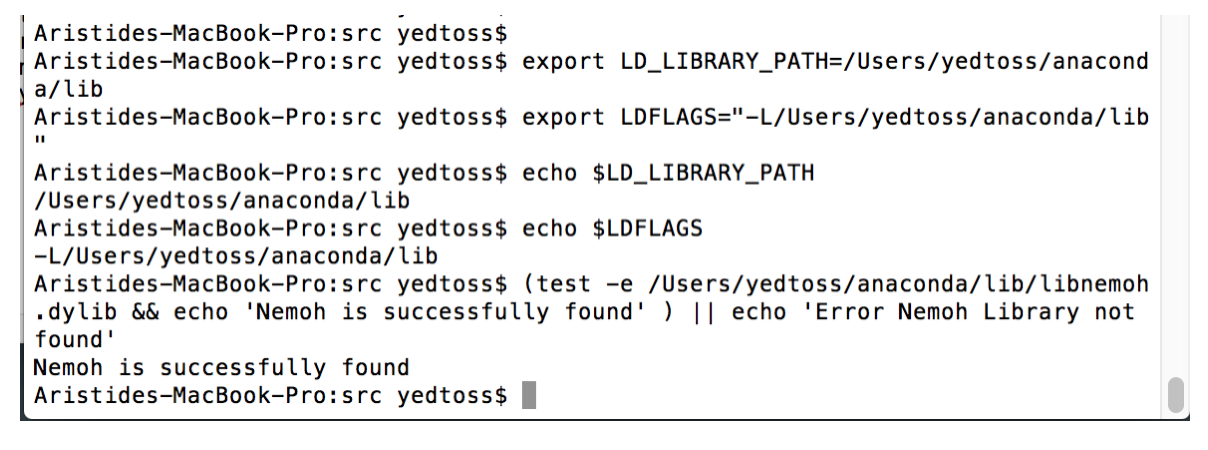
\includegraphics[scale=0.75]{img/16}
							%\captionof{figure}{Transfer from R1 to R2 whenK1=1}
						\end{minipage}
						\vspace{\belowdisplayskip}
						
						If you get an error message here, it means you did not correctly set up the path to the Nemoh library.
						
						
						\item Make sure the nglib-mesh binary is runnable:
						{\color{blue}chmod +x \ROOT/src/bundled/mesh-generator/build/nglib-mesh} 
						(Recall that \ROOT is the top-level directory of the OpenWarp package.)
						
						\item To prevent dylib errors, go to the directory \ROOT/src/bundled/mesh-generator/lib/ and run:
						
							{\color{blue}python update{\_}dylib.py}
							
								\vspace{\abovedisplayskip}
								\begin{minipage}{\linewidth}
									\centering
									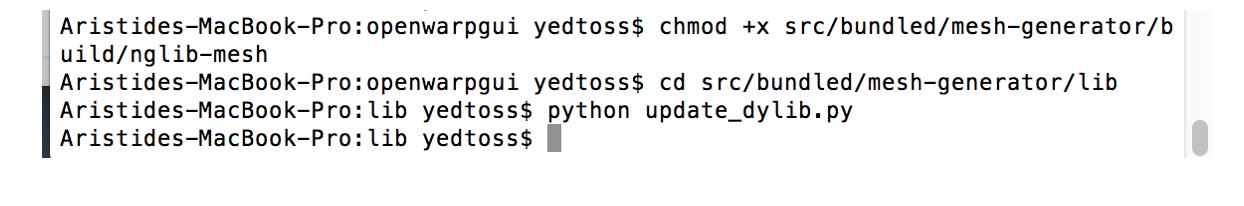
\includegraphics[scale=0.75]{img/17}
									%\captionof{figure}{Transfer from R1 to R2 whenK1=1}
								\end{minipage}
							\vspace{\belowdisplayskip}
							
						\item
						Install the remaining Python dependencies by going to \ROOT/src/ and running:
						{\color{blue}pip install -r requirements.txt}
						This step is required before running the OpenWarp server for the first time. You can skip it when running the server on subsequent occasions.
						
							\vspace{\abovedisplayskip}
							\begin{minipage}{\linewidth}
								\centering
								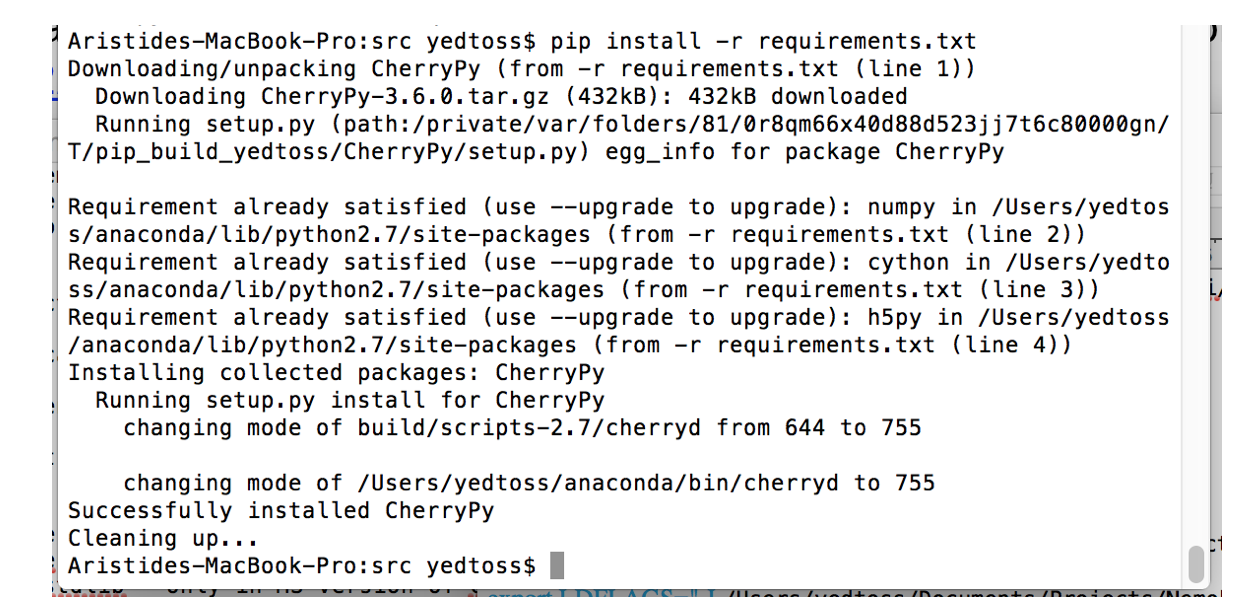
\includegraphics[scale=0.75]{img/18}
								%\captionof{figure}{Transfer from R1 to R2 whenK1=1}
							\end{minipage}
							\vspace{\belowdisplayskip}
							
							
							\item
							To start the server, run:
								{\color{blue} sudo python main.py}
							If you get an error, make sure that port 80 is not being used by another process.
							
						\vspace{\abovedisplayskip}
						\begin{minipage}{\linewidth}
							\centering
							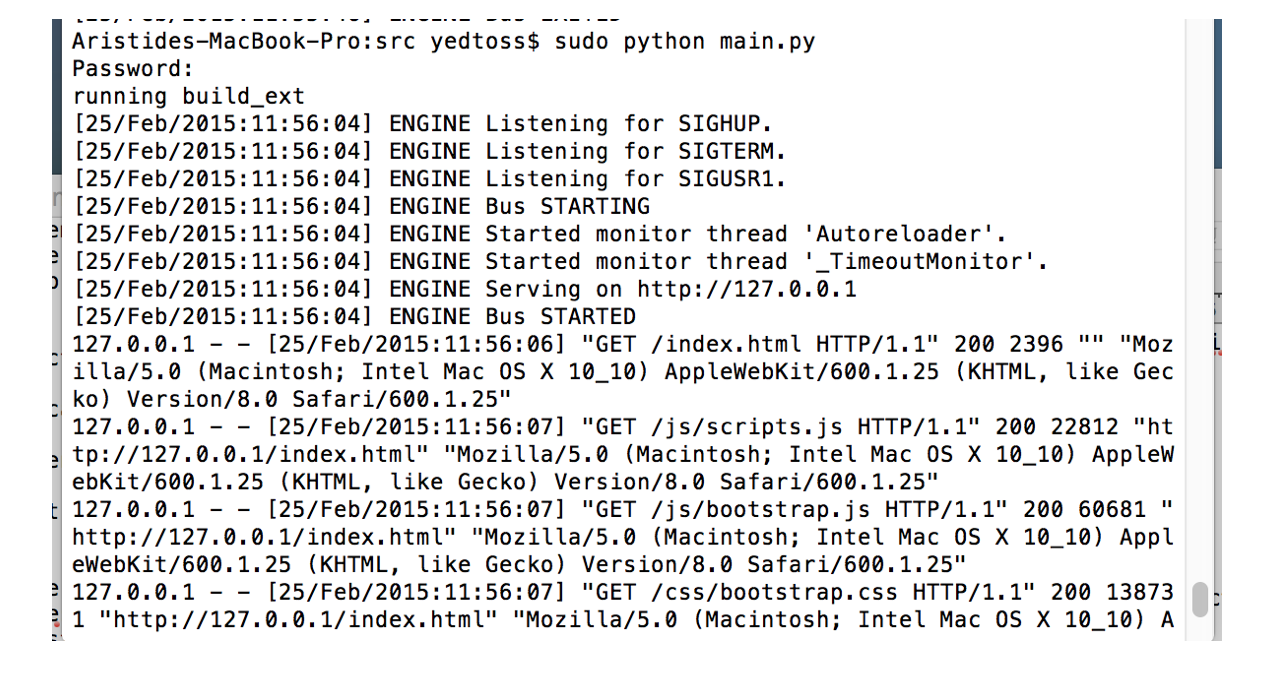
\includegraphics[scale=0.75]{img/19}
							%\captionof{figure}{Transfer from R1 to R2 whenK1=1}
						\end{minipage}
						\vspace{\belowdisplayskip}
						
						If you get an error message reading "library not found for -lnemoh" or "No module named solver{\_}fortran", make sure you have correctly exported the path to Nemoh in the current terminal session as explained earlier.
						
					
					
					
					
					
					
				
	
	
\end{itemize}


\subsection{Linux deployment from scratch}

It is enough to run the script install.sh inside \ROOT{} while being connected to the Internet. Note that you are supposed to use that script from the pre-built package of Linux as explained in \ref{prebuilt-linux}; otherwise you should download and install Paraview yourself before running the script.
Only tested on Ubuntu 14.04 64 bits.


\section{Installing the pre built package}
\label{prebuilt}
\sectionmark{from pre-built package}

Get the OpenWarp Installer from
\url{https://drive.google.com/folderview?id=0B56WkDEeFyNHfmRZNmcyZjNWOTFfTzZabGgxZVdsQUg3Y3d 6SXloWk8xMXo0bXhnSUVTOGM&usp=sharing}

The windows one is in the Windows directory. The MAC one is in the MAC directory. Note that those two installers are outdated.
The Linux one is in the Linux directory.
\subsection{OS X}

\begin{itemize}
	\item Download the MAC OS X packages and right-click on it. Then select Open in the contextual menu to install it.
\item To run the OpenWarp GUI later, go to the directory where you install it and double-click "run" or "run.sh". See section \ref{usage} of this document for more information about using the installed application.
NB:
If you get a cookie error open the url (http://127.0.0.0.1:8386/index.html) in private navigation
\end{itemize}

\subsection{Windows}

\begin{itemize}
	\item Download the Windows binary of OpenWarp and double-click on it to start the installation procedure.
 \item To run the OpenWarp GUI later go to the directory where you install it and double-click "run.bat". See section \ref{usage} of this document for more information about using the installed application.
\item NB: OpenWarp GUI is known not to work with Internet Explorer. So you must use Chrome or Firefox with the url http://127.0.0.0.1:8386/index.html.
If you get a cookie error open the url in private navigation
\end{itemize}


\subsection{Linux}
 \label{prebuilt-linux}
\begin{itemize}
	\item The Linux installation is a little different from other OS. You need to make sure you are connected to Internet the first time you want to install it at least.
\item Extract the OpenWarp GUI in a folder and in a terminal run "bash installer.sh". (You can double-click to install if you extracted it to an ext4 file system). You will be asked for your sudo password. Make sure to enter it.
\item To run the installer later on, enter the folder where you had extracted the OpenWarp and run "bash run.sh". See section \ref{usage} of this document for more information about using the installed application.
NB:
If you get a cookie error open the url (http://127.0.0.0.1:8386/index.html) in private navigation This is known to happen in some configuration of Firefox
\end{itemize}




\section{Deployment from existing package }
\sectionmark{from existing installer}

Instead of building from scratch, you can first install the old installer using section \ref{prebuilt}

Then follow these steps:

\subsection{Windows}

\subsubsection{Recompiling NemohFortran and NemohPython}
\begin{itemize}
	\item You need to make sure to replace all new codes in \INSTALLDIR/OpenWarp by the one in the submission (the new one.)
 \item Follow instructions of section \ref{ws} to build a local copy.
  Replace \NEMOHFORTRAN by \INSTALLDIR/OpenWarp/NemohImproved/Nemoh;
  
\ROOT/src should be replaced by \INSTALLDIR/OpenWarp/openwargui
The python version of nemoh should be \INSTALLDIR/OpenWarp/openwargui/nemoh Anaconda should be \INSTALLDIR/OpenWarp/Anaconda
\item  Now copy the newly generated libnemoh.dll and libnemoh.dll.a to \INSTALLDIR/OpenWarp/Anaconda/DLLs. 

\item If your code needs any additional DLLS make sure to put them there
\end{itemize}

\subsubsection{Repackaging the installer}
\begin{itemize}
	\item Copy the directory src/Windows/installer to \INSTALLDIR such that \INSTALLDIR/OpenWarp and \INSTALLDIR/installer exists.
\item Download and Install Inno Setup version equal or greater than $5.5.5$ from \url{http://www.jrsoftware.org/isdl.php}
\item Open \INSTALLDIR/installer/openwarp.iss with Inno Setup (You may double-click on the file)
\item Inno Setup will open. Click on Build --> Compile (menu). Once done the installer will be in
\INSTALLDIR/OpenWarp/installer/Output/OpenWarp.exe
\end{itemize}

\subsection{OS X}

\subsubsection{Recompiling NemohFortran and NemohPython}

\begin{itemize}
	
	 	\item You need to make sure to replace all new codes in \INSTALLDIR/OpenWarp by the one in the submission (the new one.)
	 	\item Follow instructions of section \ref*{os} to build a local copy.
	 	Replace \NEMOHFORTRAN by \INSTALLDIR/OpenWarp/NemohImproved/Nemoh;
	 	
	 	\ROOT/src should be replaced by \INSTALLDIR/OpenWarp/openwargui
	 	The python version of nemoh should be \INSTALLDIR/OpenWarp/openwargui/nemoh Anaconda should be \INSTALLDIR/OpenWarp/Anaconda
 \item Now copy the newly generated libnemoh.dylib to \INSTALLDIR/OpenWarp/anaconda/lib
\item Then {\color{red} VERY IMPORTANTLY} run in a terminal
 {\color{blue} install{\_}name{\_}tool -change "libnemoh.dylib" "../anaconda/lib/libnemoh.dylib" \INSTALLDIR/OpenWarp/openwarpgui/nemoh/solver{\_}fortran.so}  from \INSTALLDIR/OpenWarp/openwargui/nemoh
	
\end{itemize}

\subsubsection{Packaging the installer}

\begin{itemize}
	\item Copy the directory src/MAC/installer to \INSTALLDIR such that \INSTALLDIR/OpenWarp and\$INSTALLDIR/installer exists.
\item Download and install Packages (version $>= 1.1.1$) from \url{http://www.macupdate.com/app/mac/34613/packages}
\item Open \INSTALLDIR/OpenWarp/installer/OpenWarp with Packages (You can double-click on it)
\item In the menu click on Build --> Build or Type Command +B
\item The installer will start building and once done the MAC OS X packages will be in \INSTALLDIR/OpenWarp/installer/build/OpenWarp.pkg
\end{itemize}

\subsection{Linux}

Here the file installer.sh is taking care of everything. In most cases you don't have to do anything extras in case the code is updated. In any case just make sure installer.sh and run.sh are accurate and can be used to install and run the new code in a clean system.

\subsubsection{Recompiling NemohFortran and NemohPython}
Not needed as the installer.sh take care of that automatically.
\subsubsection{Packaging the installer}
You just need to compress the directory \INSTALLDIR.

\subsection{General Guide about the installer build/packaging procedure}

OpenWarp is composed of three main parts: the Fortran part of Nemoh whose source is available in \INSTALLDIR/OpenWarp/NemohImproved/Nemoh; the Python part of Nemoh whose source is available in \INSTALLDIR/OpenWarp/openwarpgui/nemoh and the OpenWarp GUI part whose source is available in \INSTALLDIR/OpenWarp/openwarpgui/openwarp.
If you do not update the Fortran part of Nemoh or the file \INSTALLDIR/OpenWarp/openwarpgui/nemoh/solver_fortran.pyx then the only step you have to do to rebuild the installer is to package it directly. There is no need to do any re-compilation steps.
When you update the Fortran or \INSTALLDIR/OpenWarp/openwarpgui/nemoh/solver_fortran.pyx you need to recompile them and copy the generated library in a well-defined location. See the relevant OS guide for more information.


In case you added some python dependencies not currently available, you would need to package them in the installer. For Linux you can update the relevant \INSTALLDIR/OpenWarp/openwarpgui /requirements.txt and it will be installed automatically by \INSTALLDIR/OpenWarp/installer.sh

For Windows and MAC OS X you would need to install those dependencies in the provided Anaconda site-packages available in \INSTALLDIR/OpenWarp/Anaconda and \INSTALLDIR/OpenWarp/anaconda respectively.
If you add some external libraries as dependencies you need to make sure they are available to end users. In Windows you can just copy them to \INSTALLDIR/OpenWarp/Anaconda/DLLs.

In MAC OS X you can just copy them to \INSTALLDIR/OpenWarp/anaconda/lib. Make sure there are static or update their dependencies using install_name_tool (You can see an example in the MAC OS X specific instructions).
For Linux/Ubuntu, it is preferred to use apt-get install to make those external libraries available to end users.

\section{Configuration}
The three parts of the application can all be configured using the web application GUI. In this section, we describe the configurable parameters for each part.

\subsection{Meshing parameters}

\begin{description}
	\item [Input File]: This is the input file geometry for which we want to generate quadrilateral elements. The accepted input file formats are IGS, STEP, and STL.
\item [Output File]: Enter the name of the output file without any file extension. This should be a bare file name without a directory path preceding it.
\item [Fineness]: The target fineness of the mesh.
\item [MaxH]: The maximum height of the quadrilateral elements in the mesh. 
\item [MinH]: The minimum height of the quadrilateral elements in the mesh. 
\item [Grading]: The grading of the mesh.
\item [Use Tolerance]?: Whether or not to use tolerance when generating the mesh. When the absolute value of the difference between two values is less than the tolerance, we consider them to be equal.
\item [Tolerance]: Volume tolerance expressed as a number from 0 to 1.
\end{description}


\subsection{Simulation parameters}

\begin{description}
	\item []
	\item [Rho]: The fluid's specific volume in $KG/m^3$.
\item [G]: Gravity in $m/s^2$.
\item [Depth]: The depth of the water in meters. Enter 0 to indicate infinite depth.
\item [XEFF, YEFF]: The x and y coordinates, in meters, of the point where the wave is measured.
\item [Name of Mesh File]: The name of the mesh file generated in the meshing step.
\item [Number of Points and Number of Panels]: The number of points in the mesh and the total number of panel or quadrilaterals in the mesh. These values are automatically filled in.
\item [Surge:] The freedom of translation along the X axis (moving forward and backward).
\item [Sway]: The freedom of translation along the Y axis (moving left and right).
\item [Heave]: The freedom of translation along the Z axis (moving up and down).
\item [Roll About A Point]: The freedom of rotation along the X axis (pivoting side to side).
\item [Pitch About A Point]: The freedom of rotation along the Y axis (tilting forward and backward).
\item [Yaw About A Point]: The freedom of rotation along the Z axis (swiveling left and right). 
\item [Force In X, Y, Z Direction]: Three-dimensional coordinates of force.
\item [Moment Force In X, Y, Z Direction About A Point]: Three-dimensional coordinates of moment force.
\item [Number of Lines of Additional Information] Currently not supported. Should be set to 0.
\item [Number of Wave Frequencies, MIN, MAX]: Respectively the number of wave frequencies, the minimum value of each wave frequency, and the maximum value of each wave frequency.
\item [Number of Wave Directions, MIN, MAX]: Respectively the number of wave directions, the minimum value of each wave direction, and the maximum value of each wave direction.


\item [Indiq{\_}solver]: The method to use for solving linear equation. Use 0 to indicate the Gauss Method, 1 to indicate the GMRES method, and 2 to indicate the GMRES method with FMM acceleration. Option 2 is not yet supported.
\item [TOL_GMRES] : The value of the tolerance to use for the GMRES method. The tolerance is used to determine convergence.
IRES : Restart parameter for GMRES. MAXIT: Maximum iterations for GMRES.
\item [Sav_potential] : Use 0 or 1 to indicate whether or not the potential should be saved in the output.

\item [GREEN_TABULATION_NUMX] : Represents the number of points in the X direction in the tabulated data.
\item [GREEN_TABULATION_NUMZ]: Represents the number of points in the Z direction in the tabulated data.
\item [GREEN_TABULATION_SIMPSON_NPOINTS]: Represents the number of sub-intervals used to approximate the Green's function integral using Simpson's rule.
\item [USE_ODE_INFLUENCE_COEFFICIENTS] Indicate whether or not to use the ODE method to compute the influence coefficients.
\item [USE_HIGHER_ORDER]: Whether or not to use the higher-order panel method. 
\item [NUM_PANEL_HIGHER_ORDER]: The number of panels per patch in the higher-order
method.
\item [B_SPLINE_ORDER]: The order of the B-spline for the potential in the higher-order panel method.
\item [USE_DIPOLES_IMPLEMENTATION]: Whether or not to use the dipole implementation. 
\item [THIN_PANELS]: A list containing the indices of panels which are thin dipoles. Indices
are zero-based. Set the list to [-1] to indicate that all panels are thin dipoles. 
\item [COMPUTE_DRIFT_FORCES]: Whether or not to compute the drift forces. 
\item [COMPUTE_YAW_MOMENT]: Whether or not to compute the yaw moment.
\end{description}


\subsection{Postprocessing parameters}

\begin{description}
	\item [ IRF]: Whether or not to compute the IRF, i.e., the infinite frequency added mass and the impulse response function for the radiation force.
\item [TIME Step]: The time step used for the IRF computation.
\item [Duration]: The duration used for the IRF computation.
\item [Show Pressure]: Whether or not to output the pressure forces.
\item [Kochin Function]: The number of angles to use in computing the Kochin function. Set 0 to disable this computation.
\item [Min Angle, Max Angle]: The minimum and maximum angle to use in computing the Kochin function.
\item [Number of Points In X, Y Direction]: Number of points in each direction for the free- surface visualization. Set 0 to disable the computation.
\item [Dimensions of Domain In X, Y Direction]: The domain dimension in each direction, in degrees.
\end{description}


\subsection{Other and Logging parameters}

There are only two parameters currently for the Configuration screen and they all support logging. We have:

\begin{description}
	\item [Logging level]:  Pick "DEBUG" or "INFO" to set the logging level to the respective value
	
	\item [Clear old logs]: Whether or not to delete the old log files
\end{description}

The logging level can also be configured using the configuration file \NEMOHPYTHON{}/logging.json

When run from the web interface the logs are located by default in the user home in OpenWarpFiles/logs

When run from the command line the logs are located in the configured base test directory in 
\NEMOHPYTHON{}/settings.py




\section{Usage}
\label{usage}


\subsection{Start the application}
Make sure the server has been started:
{ \color{blue} python main.py}
This command must be executed from the \ROOT/source/openwarpgui directory
Open a web browser and go to:
\url{http://127.0.0.1/index.html}
You will see the following.

\begin{itemize}
	\item To launch the application on Windows, go to where you have installed it (by default C:/Program Files (x86)/OpenWarp) and double-click "run.bat"
	
	You can then access the GUI using the url \url{http://127.0.0.0.1:8386/index.html}
	
	Don't use Internet Explorer as it is known not to work with the GUI.
	
	
	\item To launch the application on Linux, go to where you have installed it (The directory where you extracted the archive) from a terminal and run "bash run.sh"
	You can then access the GUI using the url http://127.0.0.0.1:8386/index.html
	
	
	\item To launch the application on MAC OS X, go to where you have installed it (by default /Applications/OpenWarp) and double-click on "run" file
	You can then access the GUI using the url http://127.0.0.0.1:8386/index.html
\end{itemize}

	\vspace{\abovedisplayskip}
	\begin{minipage}{\linewidth}
		\centering
		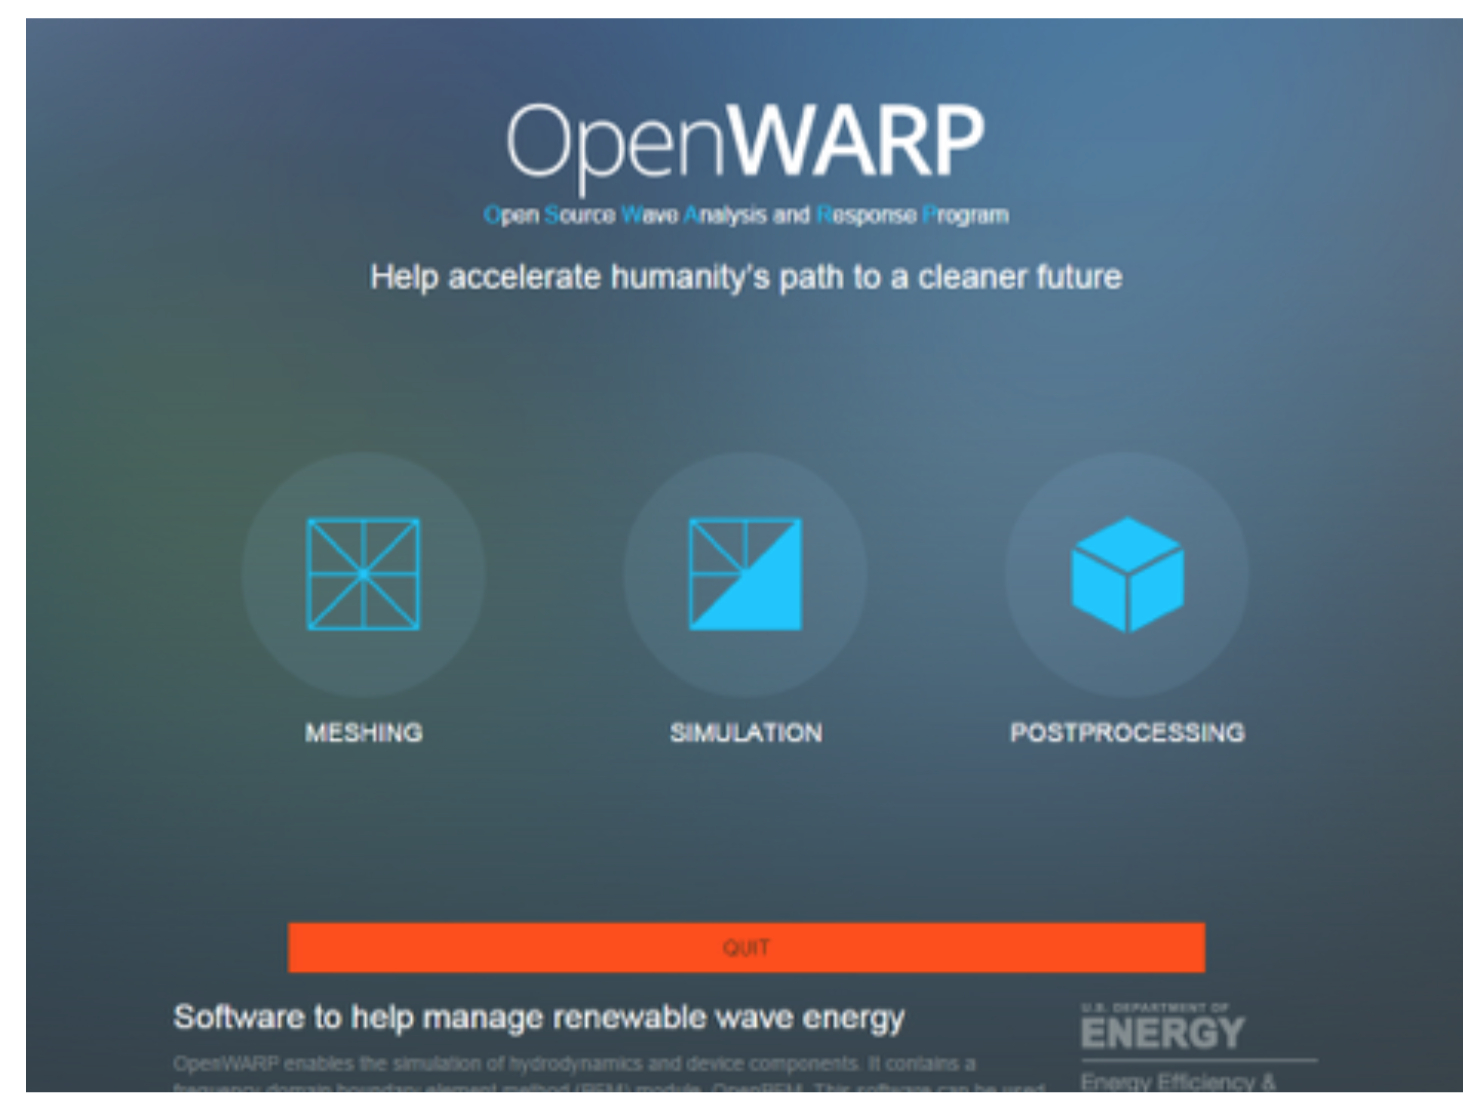
\includegraphics[scale=0.4]{img/20}
		%\captionof{figure}{Transfer from R1 to R2 whenK1=1}
	\end{minipage}
	\vspace{\belowdisplayskip}
	
	You can quit the application by clicking the orange Quit button. Quitting results in:
	
		\vspace{\abovedisplayskip}
		\begin{minipage}{\linewidth}
			\centering
			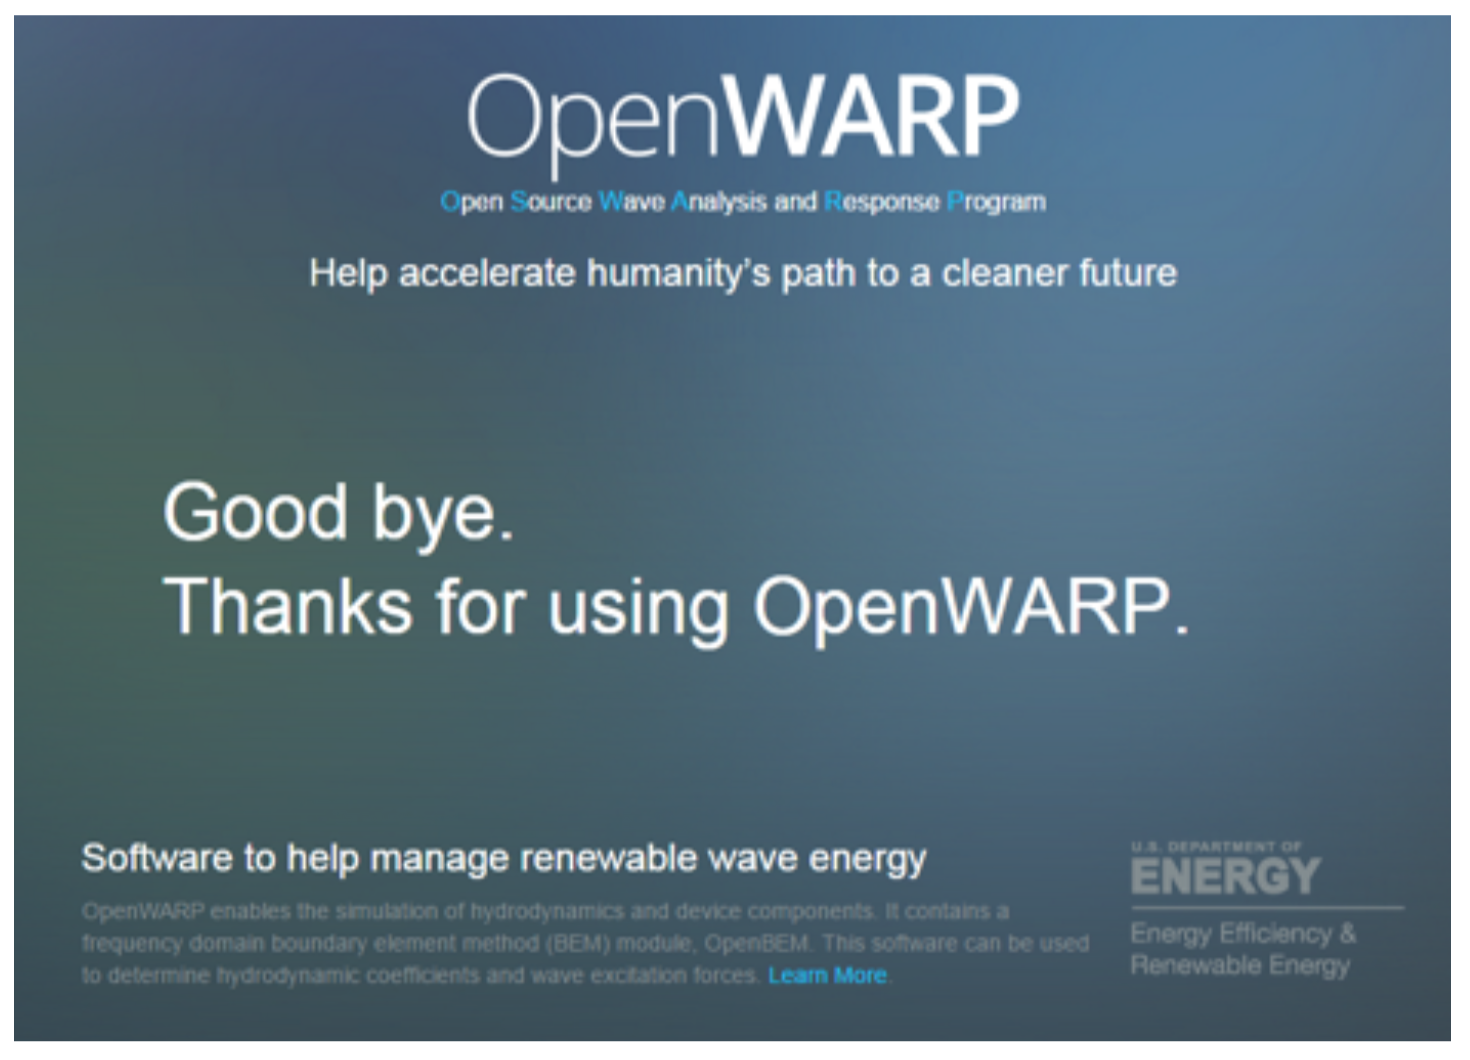
\includegraphics[scale=0.5]{img/21}
			%\captionof{figure}{Transfer from R1 to R2 whenK1=1}
		\end{minipage}
		\vspace{\belowdisplayskip}
		
		You must restart the Python server before using the application again.
		\subsection{Start meshing}
		Click the Meshing button:
		
			\vspace{\abovedisplayskip}
			\begin{minipage}{\linewidth}
				\centering
				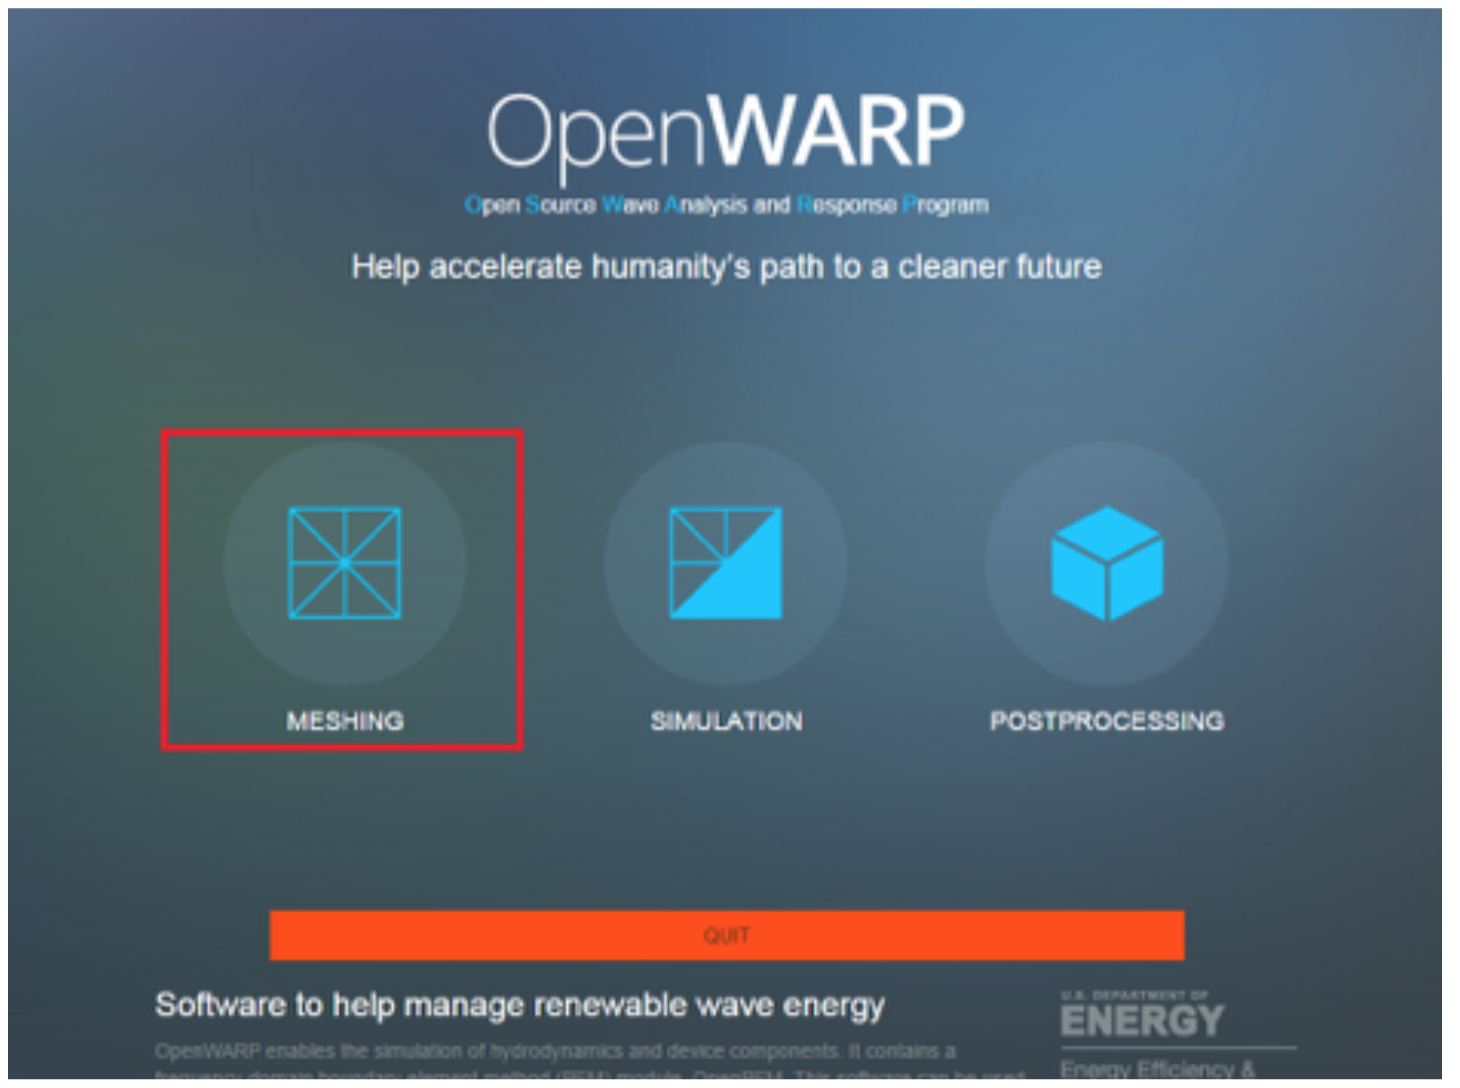
\includegraphics[scale=0.4]{img/22}
				%\captionof{figure}{Transfer from R1 to R2 whenK1=1}
			\end{minipage}
			\vspace{\belowdisplayskip}
			
			This is the meshing page:
			
				\vspace{\abovedisplayskip}
				\begin{minipage}{\linewidth}
					\centering
					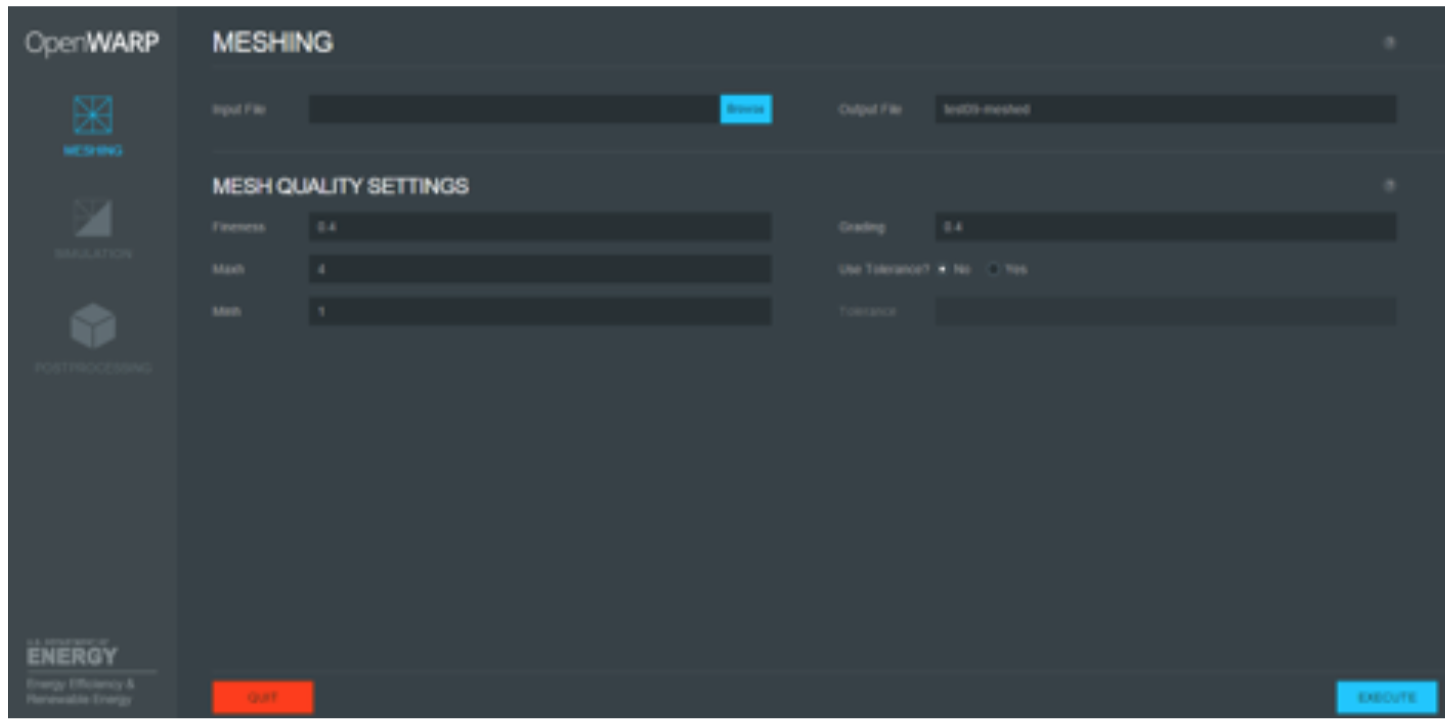
\includegraphics[scale=0.4]{img/23}
					%\captionof{figure}{Transfer from R1 to R2 whenK1=1}
				\end{minipage}
				\vspace{\belowdisplayskip}
				
				Select the input file by clicking Browse and selecting a file. Set the other parameters according to your needs.
				
				
	\subsection{Execute meshing}
	Click the blue Execute button.
	
	\subsection{View the meshing results}
	Once meshing is complete, you will see a popup displaying a log:
	
	\vspace{\abovedisplayskip}
	\begin{minipage}{\linewidth}
		\centering
		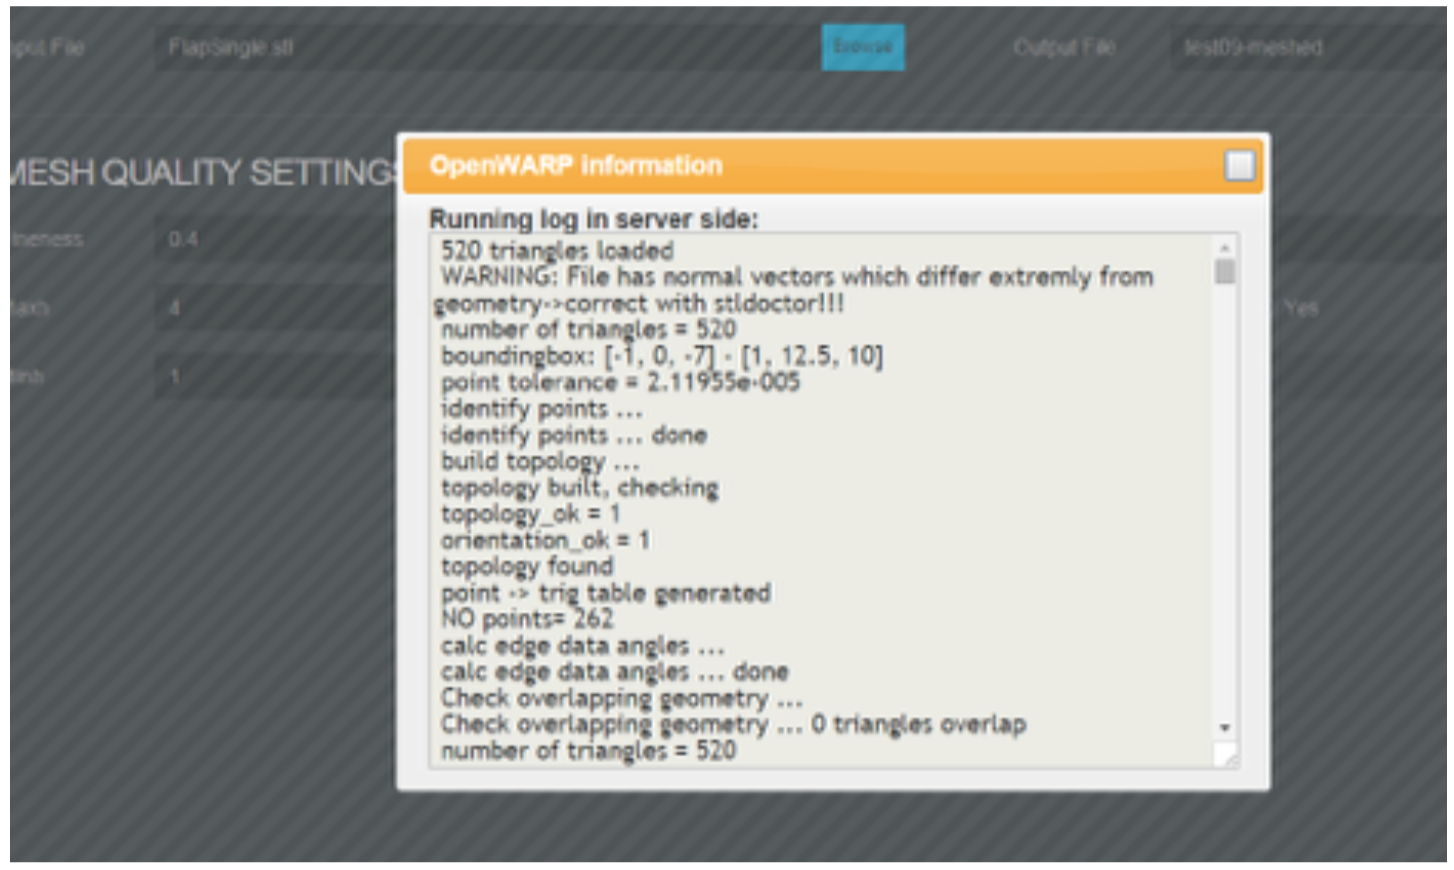
\includegraphics[scale=0.4]{img/24}
		%\captionof{figure}{Transfer from R1 to R2 whenK1=1}
	\end{minipage}
	\vspace{\belowdisplayskip}
	
	The meshing converts the input file to all formats recognised by the application. It salso convert the input file to a mesh containing only quadrilateral elements without any triangle.
The output directory is \ROOT/src/user_data/meshing_TIMESTAMP_HASH where 
\ROOT is the top-level directory of the OpenWarp package.
The timestamp is in the format YYYYMMDDHHMM. Navigate to the directory with the latest timestamp. Inside the directory, you will find:
\begin{itemize}
	\item Two files ending in .vtp, containing the mesh in VTP format. The "quad" version contains only quadrilateral elements.
	\item Two files ending in .vtk, containing the mesh in VTK format. 
	\item Two files ending in .dat, the format recognized by Nemoh. 
	
	\item 
	Two files ending in .gdf, containing the mesh in GDF format. 
	\item Two files ending in .stl, containing the mesh in stl format.
\end{itemize}

Each file is named OUTPUT_FILE_NAME.EXTENSION or OUTPUT_FILE_NAME-quad.EXTENSION, where OUTPUT_FILE_NAME is the output file name configured before meshing and EXTENSION corresponds to the file format.
For each pair of files, the "quad" version contains only quadrilateral elements.


\subsection{Start the simulation}
Click the Simulation button:

\vspace{\abovedisplayskip}
\begin{minipage}{\linewidth}
	\centering
	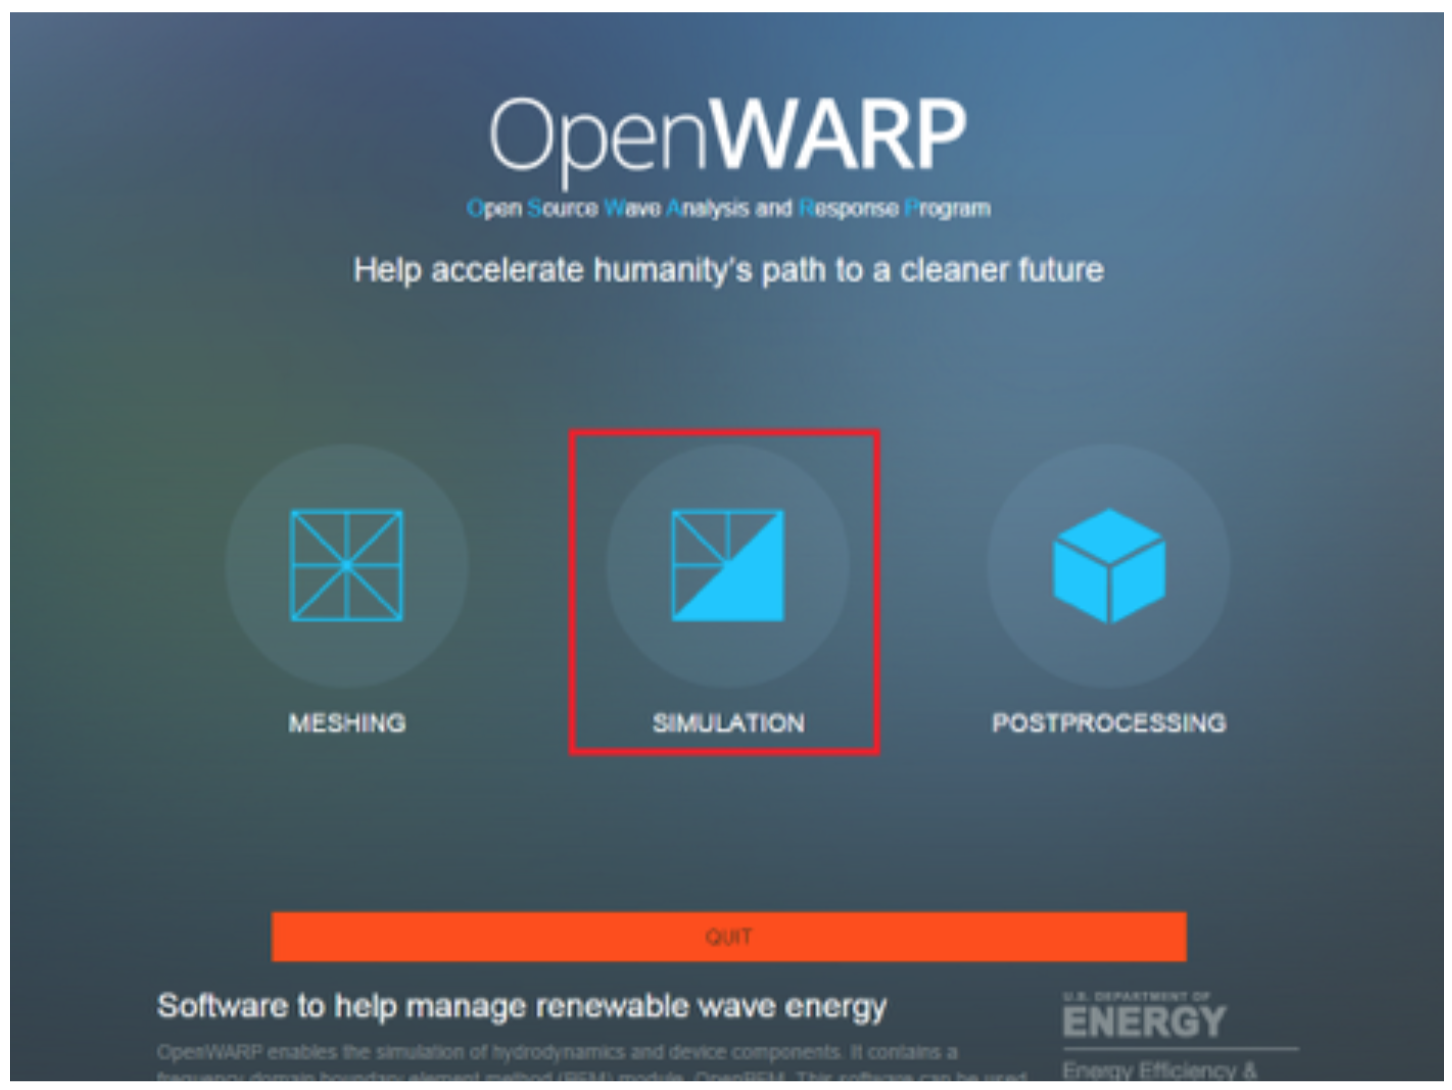
\includegraphics[scale=0.4]{img/25}
	%\captionof{figure}{Transfer from R1 to R2 whenK1=1}
\end{minipage}
\vspace{\belowdisplayskip}

This is the resulting page:

\vspace{\abovedisplayskip}
\begin{minipage}{\linewidth}
	\centering
	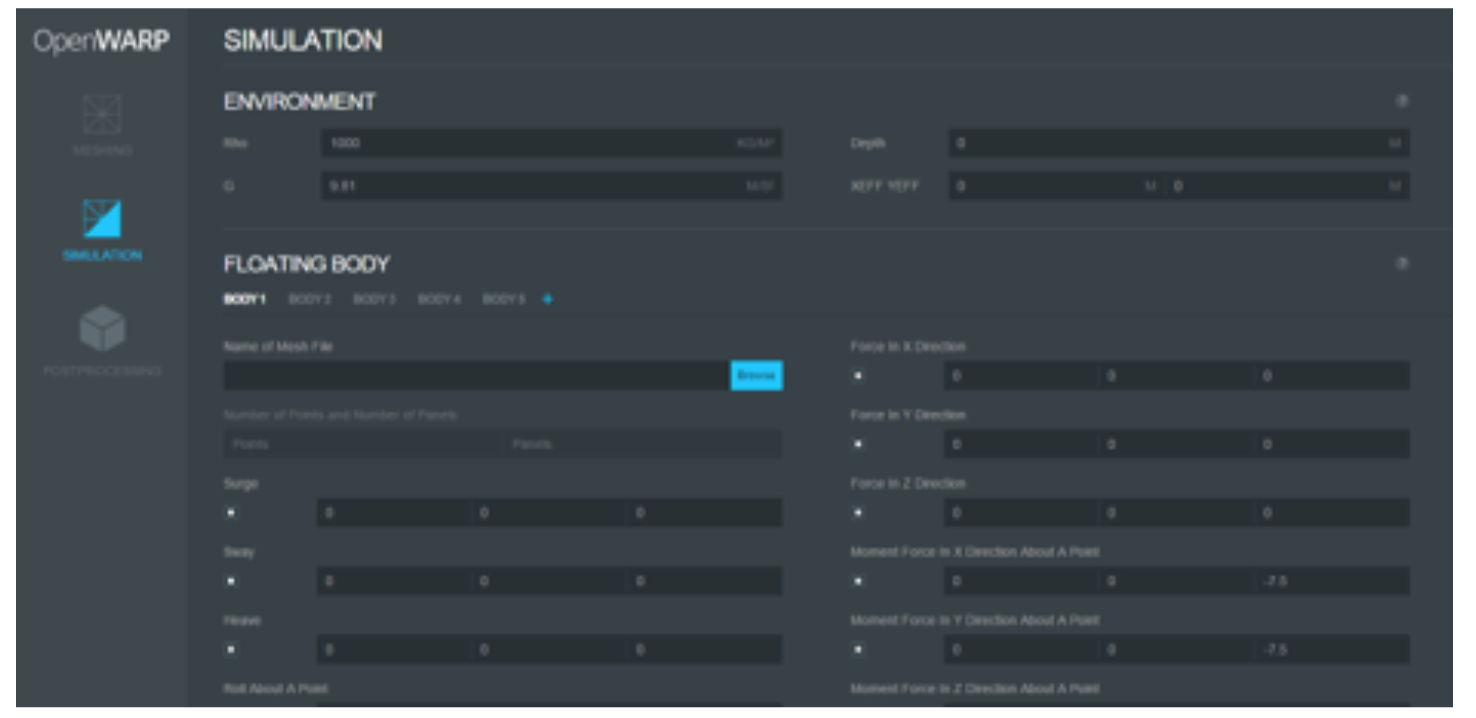
\includegraphics[scale=0.4]{img/26}
	%\captionof{figure}{Transfer from R1 to R2 whenK1=1}
\end{minipage}
\vspace{\belowdisplayskip}

\vspace{\abovedisplayskip}
\begin{minipage}{\linewidth}
	\centering
	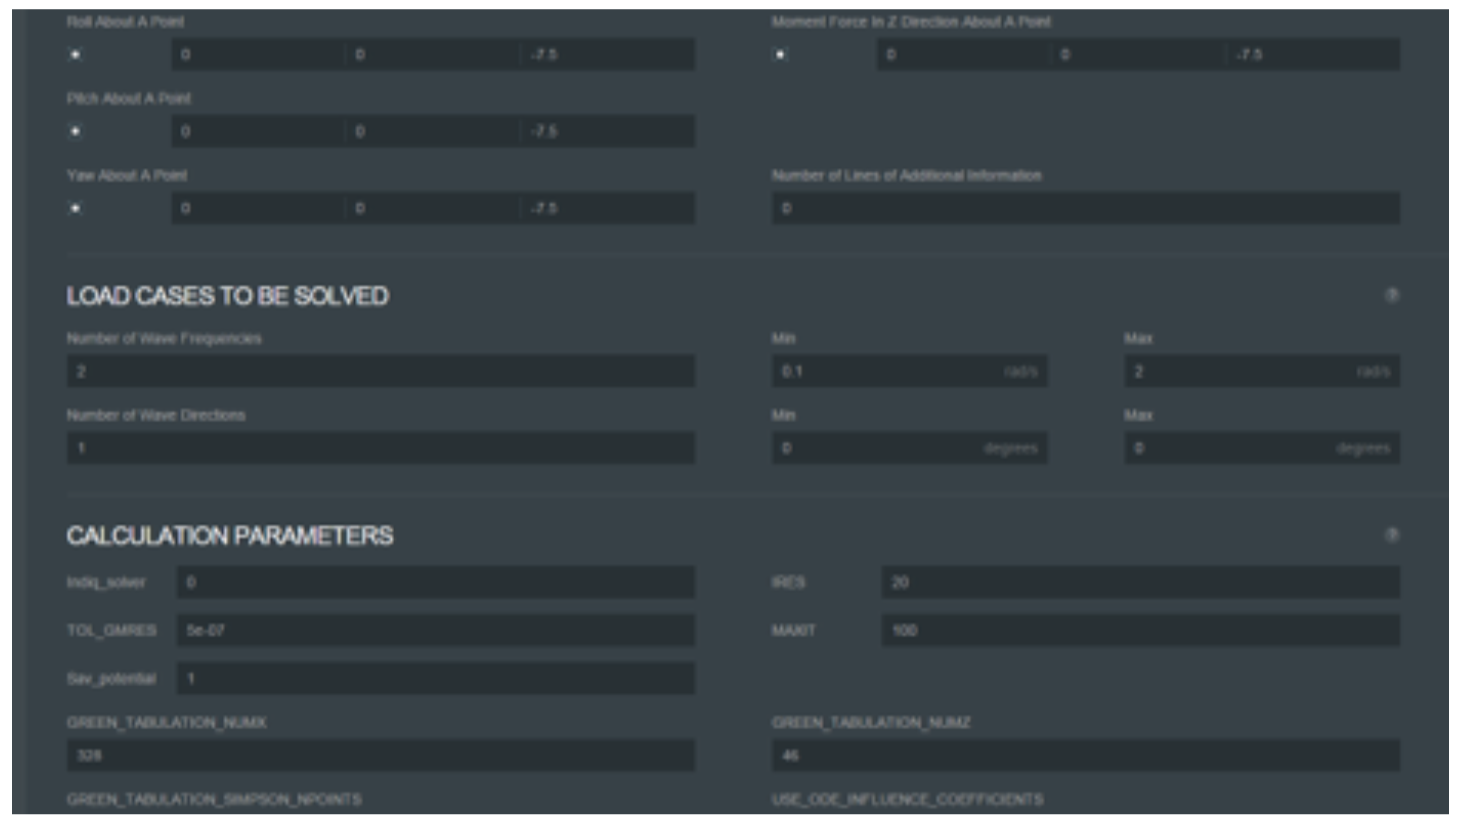
\includegraphics[scale=0.4]{img/27}
	%\captionof{figure}{Transfer from R1 to R2 whenK1=1}
\end{minipage}
\vspace{\belowdisplayskip}

\vspace{\abovedisplayskip}
\begin{minipage}{\linewidth}
	\centering
	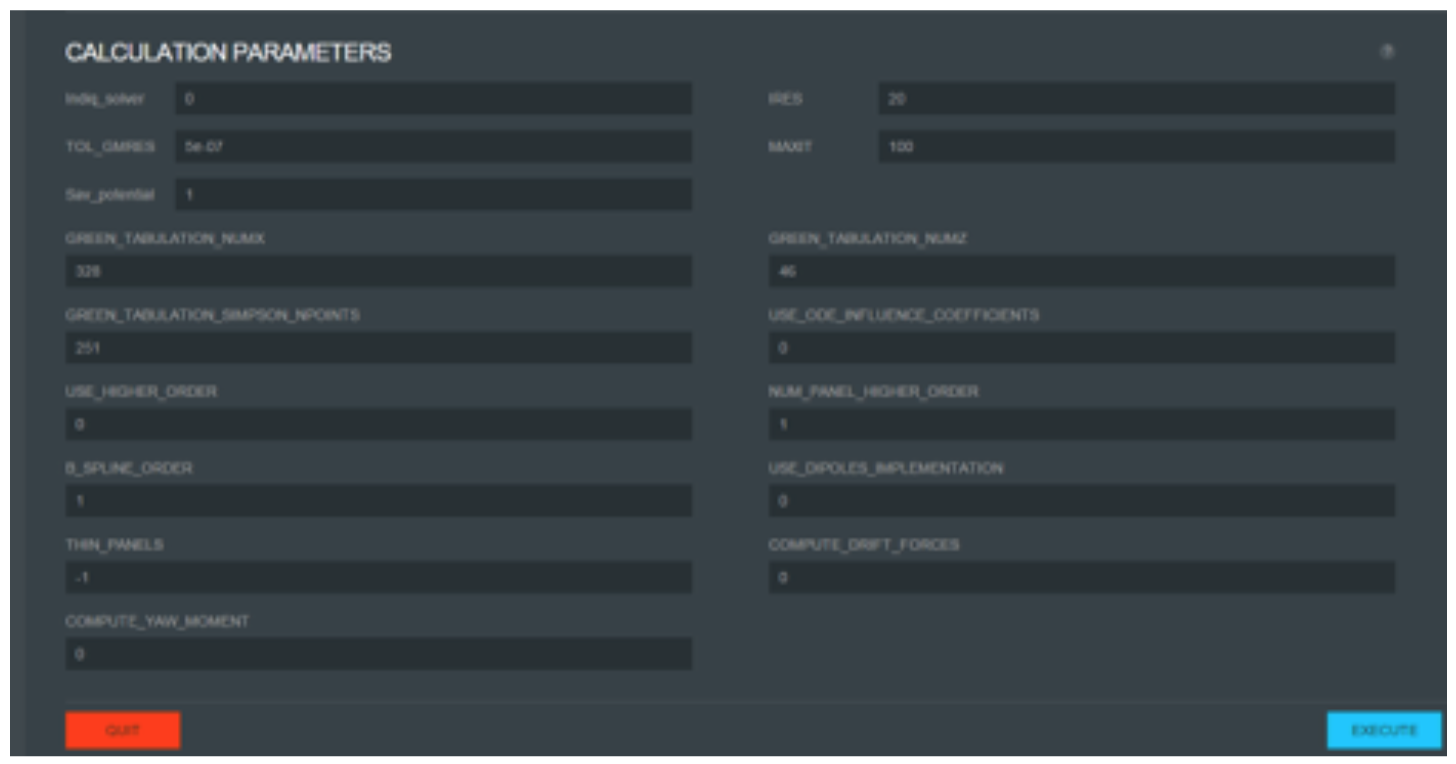
\includegraphics[scale=0.4]{img/28}
	%\captionof{figure}{Transfer from R1 to R2 whenK1=1}
\end{minipage}
\vspace{\belowdisplayskip}

\subsection{ Execute the simulation}
Click the Execute button at the bottom right of the page.

\vspace{\abovedisplayskip}
\begin{minipage}{\linewidth}
	\centering
	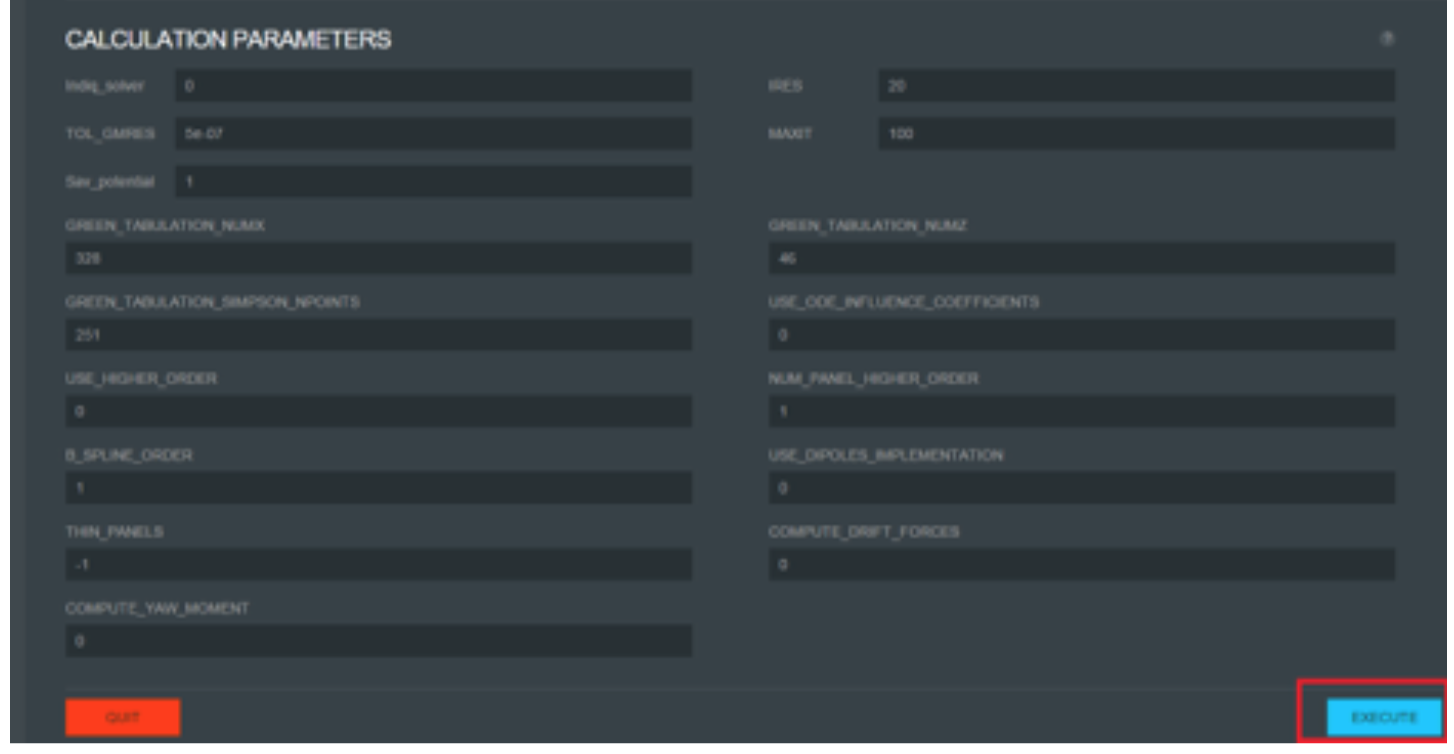
\includegraphics[scale=0.4]{img/29}
	%\captionof{figure}{Transfer from R1 to R2 whenK1=1}
\end{minipage}
\vspace{\belowdisplayskip}




\subsection{View the simulation results}
Once the simulation has completed, you will see a popup containing the calculation log:

\vspace{\abovedisplayskip}
\begin{minipage}{\linewidth}
	\centering
	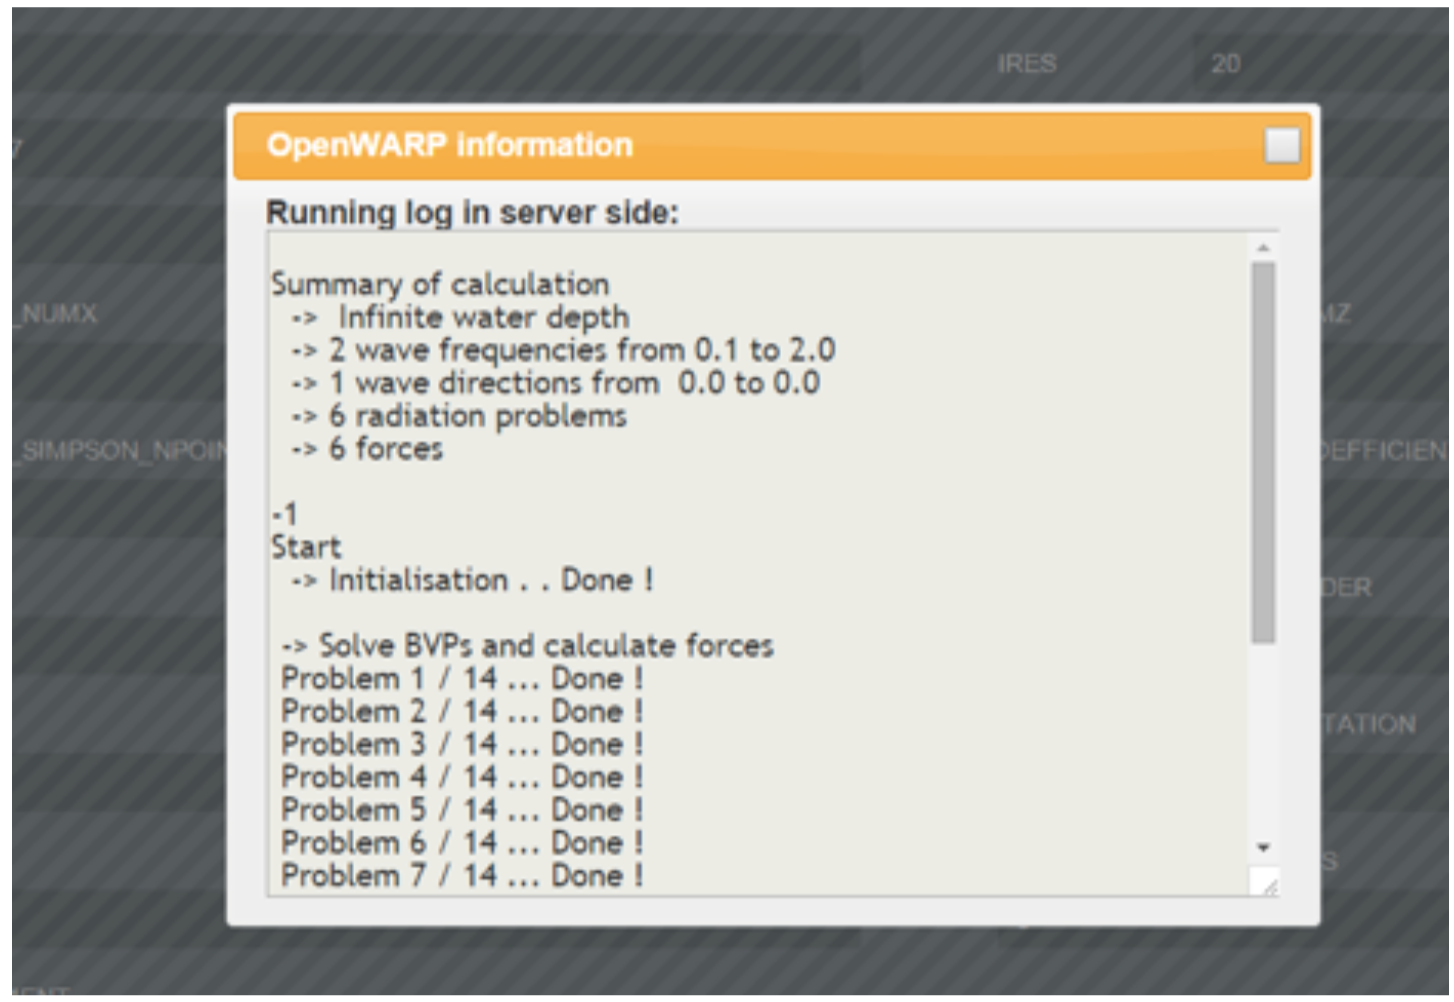
\includegraphics[scale=0.4]{img/30}
	%\captionof{figure}{Transfer from R1 to R2 whenK1=1}
\end{minipage}
\vspace{\belowdisplayskip}

The output directory is \ROOT/src/user_data/simulation_TIMESTAMP_HASH where \ROOT is the top-level directory of the OpenWarp package.
The timestamp is in the format YYYYMMDDHHMM. Navigate to the directory with the latest timestamp.
The main result at this step is the db.hdf5 file inside that directory. You can open it with HDFView:

\vspace{\abovedisplayskip}
\begin{minipage}{\linewidth}
	\centering
	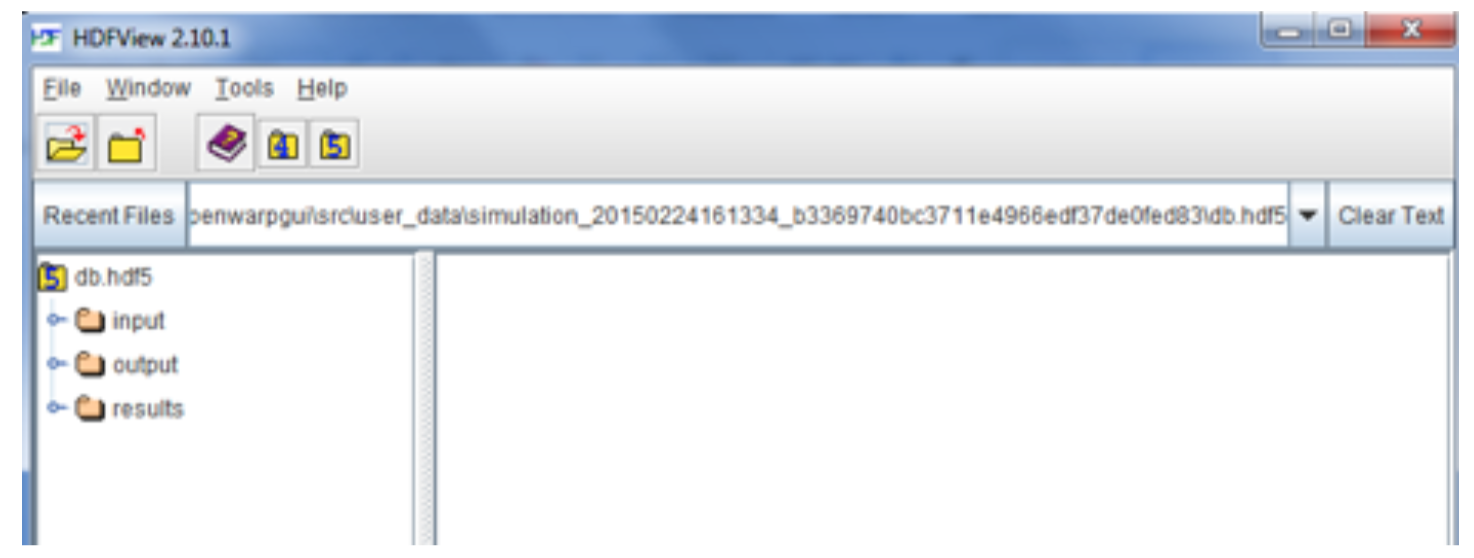
\includegraphics[scale=0.6]{img/31}
	%\captionof{figure}{Transfer from R1 to R2 whenK1=1}
\end{minipage}
\vspace{\belowdisplayskip}

You will see that it contains three main groups: the input group, the output group containing intermediate results generated by the application, and the results group containing final results. In each group, you can see datasets with their description as shown in the figure below.

\vspace{\abovedisplayskip}
\begin{minipage}{\linewidth}
	\centering
	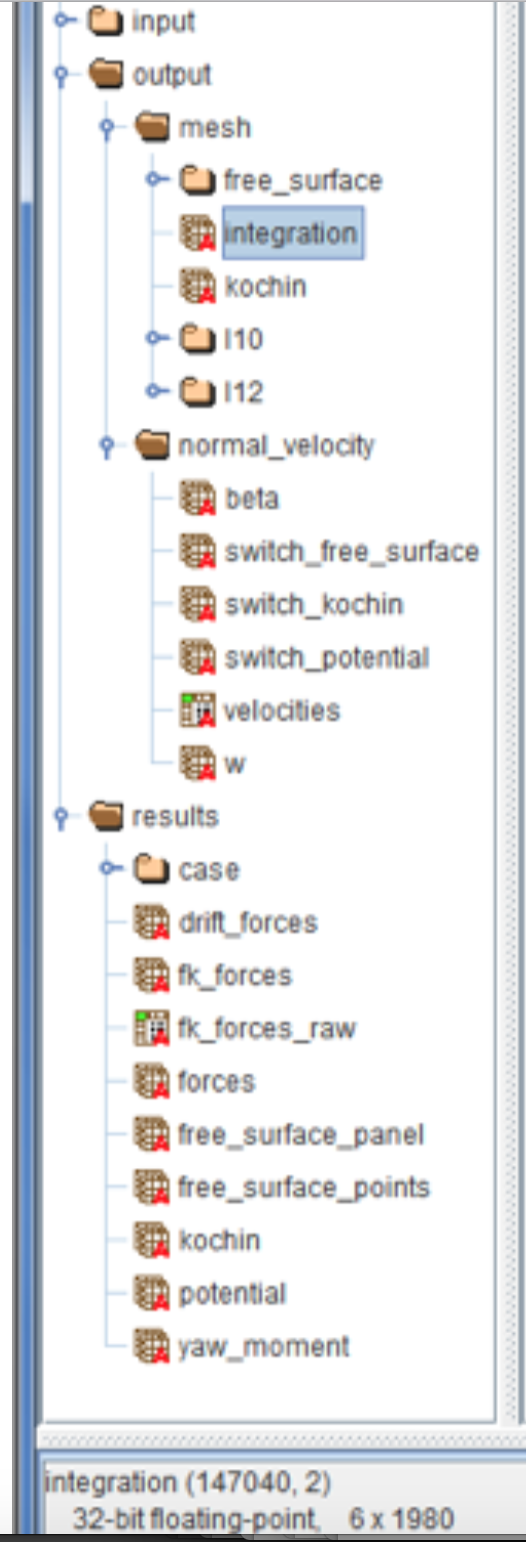
\includegraphics[scale=0.5]{img/32}
	%\captionof{figure}{Transfer from R1 to R2 whenK1=1}
\end{minipage}
\vspace{\belowdisplayskip}

\subsection{Postprocessing}
Click the Postprocessing button:

\vspace{\abovedisplayskip}
\begin{minipage}{\linewidth}
	\centering
	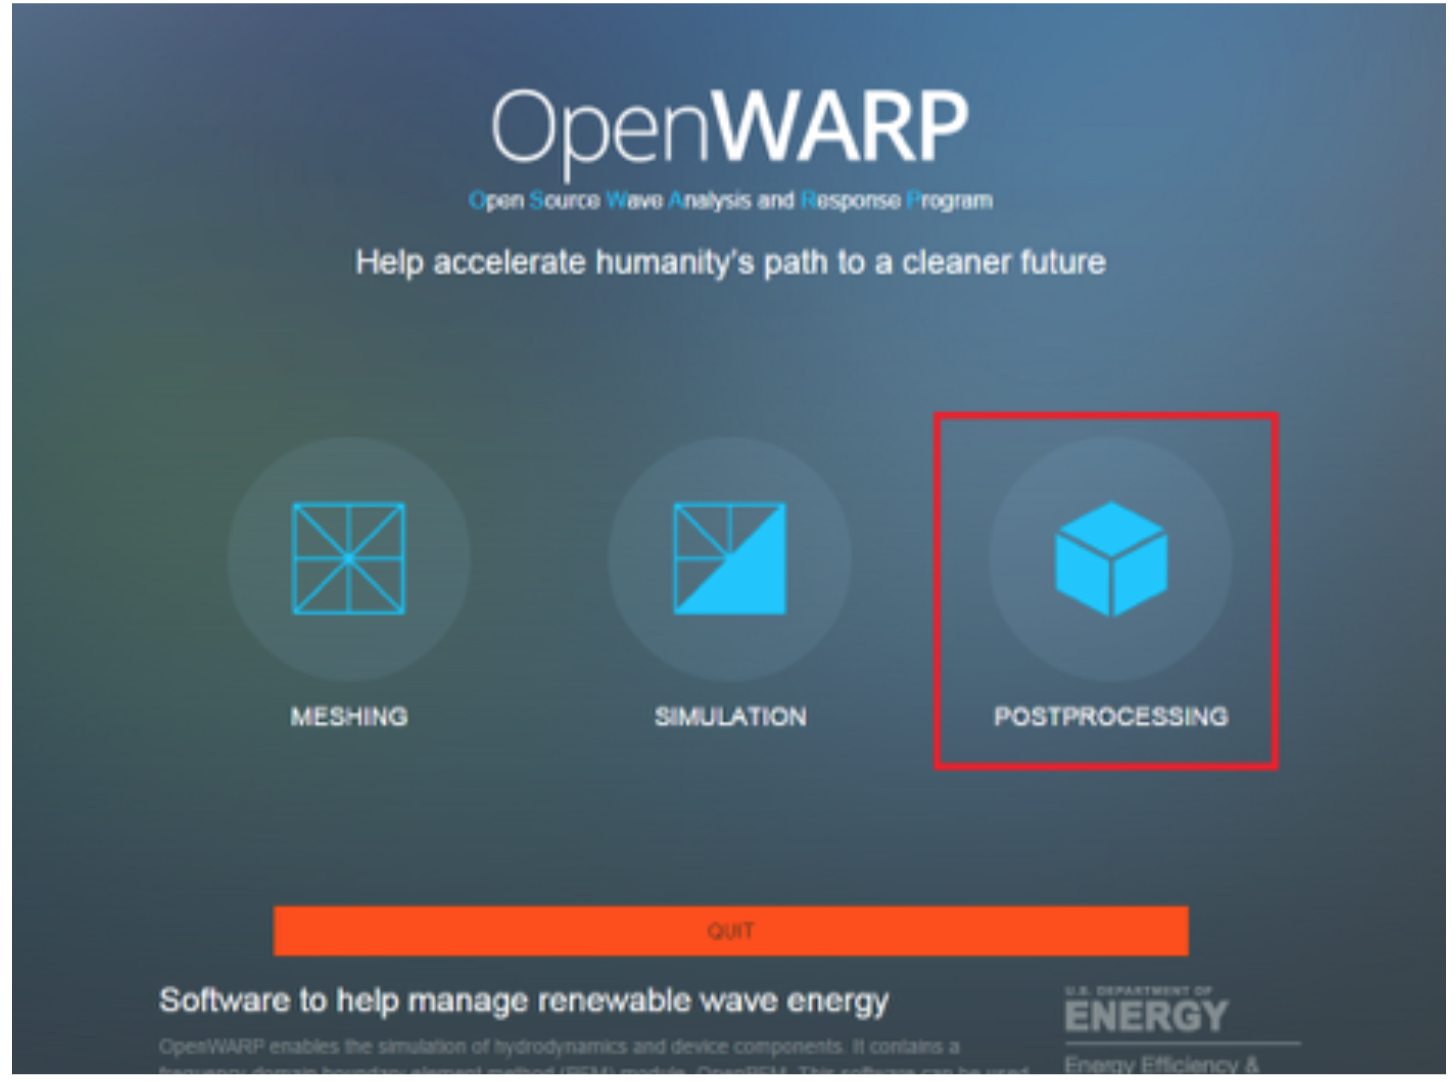
\includegraphics[scale=0.4]{img/33}
	%\captionof{figure}{Transfer from R1 to R2 whenK1=1}
\end{minipage}
\vspace{\belowdisplayskip}

You should see the following:

\vspace{\abovedisplayskip}
\begin{minipage}{\linewidth}
	\centering
	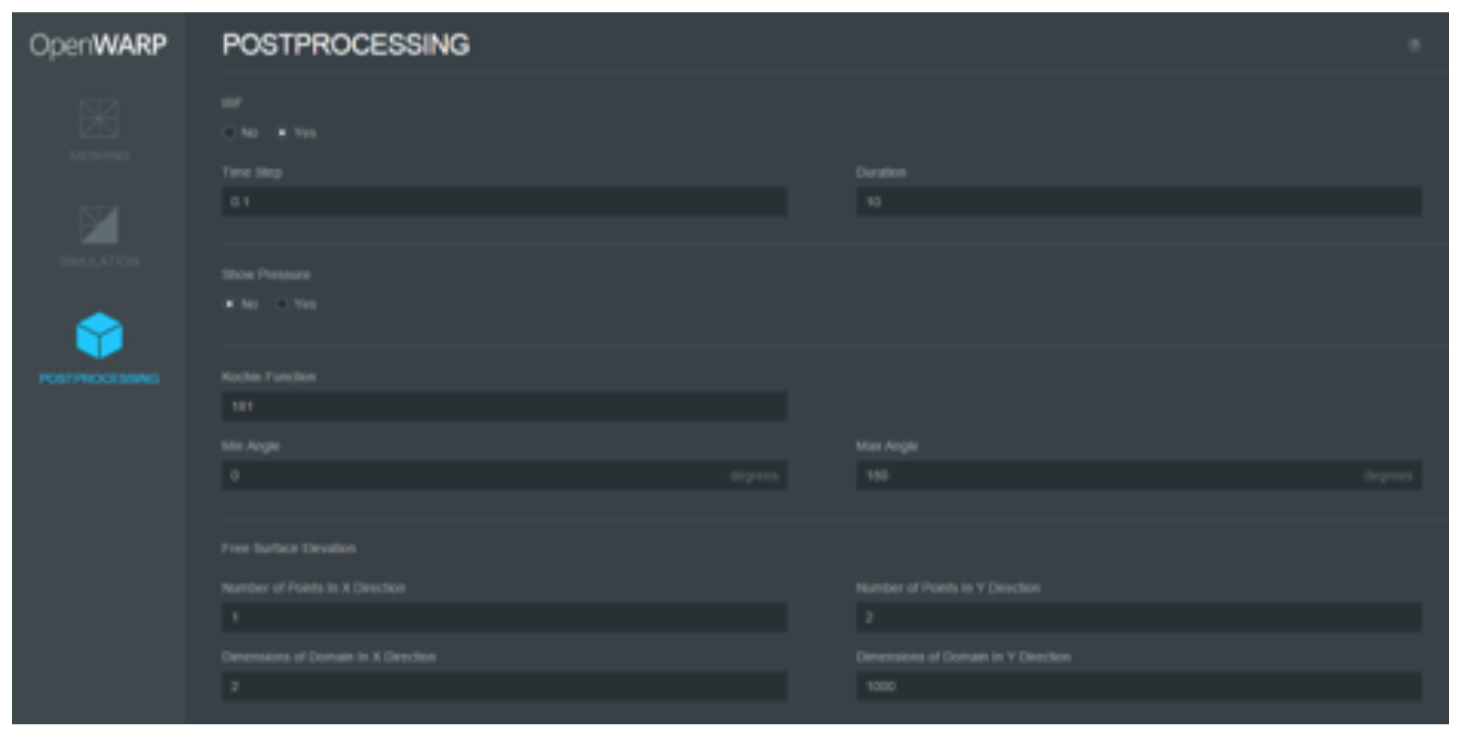
\includegraphics[scale=0.4]{img/34}
	%\captionof{figure}{Transfer from R1 to R2 whenK1=1}
\end{minipage}
\begin{minipage}{\linewidth}
	\centering
	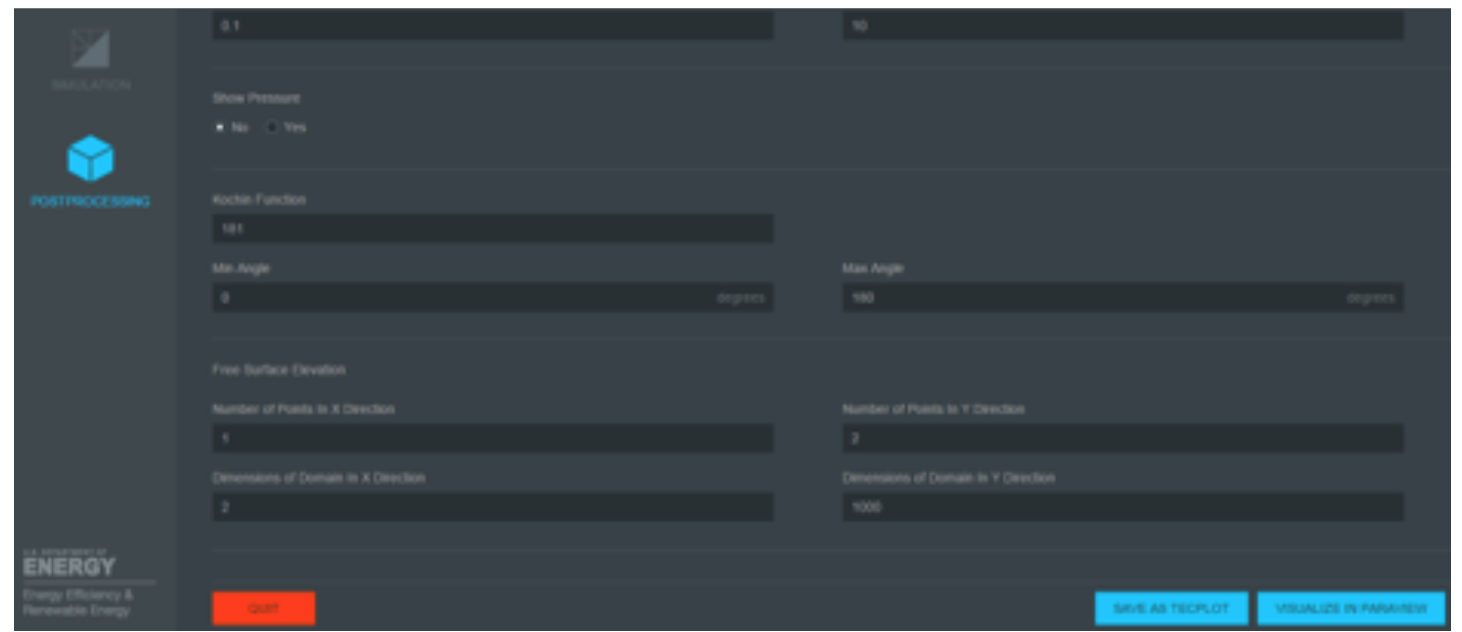
\includegraphics[scale=0.4]{img/35}
	%\captionof{figure}{Transfer from R1 to R2 whenK1=1}
\end{minipage}



\subsection{Generate TEC outputs}

Generate the TEC file by clicking on "SAVE AS TECPLOT". Note that before generating a TEC file, you must have executed a simulation in the current session.

\vspace{\abovedisplayskip}
\begin{minipage}{\linewidth}
	\centering
	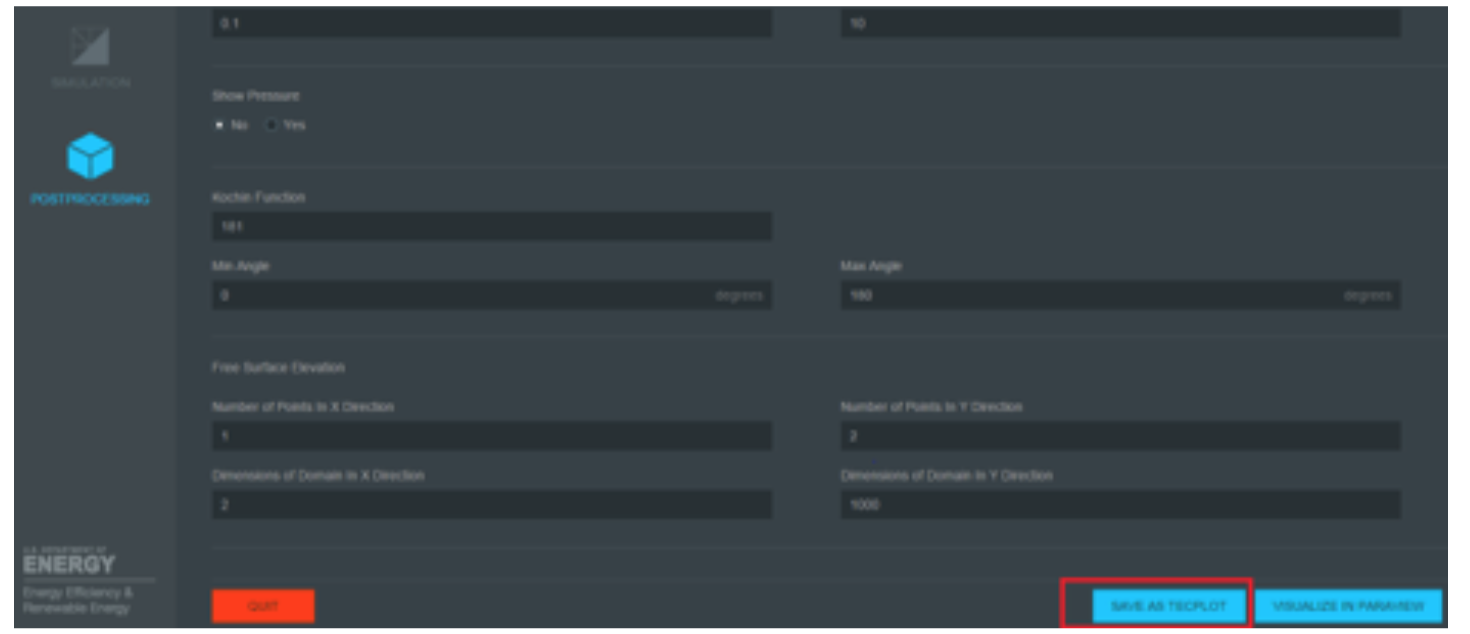
\includegraphics[scale=0.4]{img/36}
	%\captionof{figure}{Transfer from R1 to R2 whenK1=1}
\end{minipage}
\vspace{\belowdisplayskip}

\subsection{Postprocessing results}
Once the postprocessing is done, you can manually examine the results in the output directory \ROOT/src/user_data/simulation_TIMESTAMP_HASH where \ROOT is the top-level directory of the OpenWarp package.
The timestamp is in the format YYYYMMDDHHMM. Navigate to the directory with the latest timestamp. You will find the following output files:


\begin{description}
	\item [results/irf.tec]: This file contains the infinite frequency added mass and the impulse response function for the radiation force.
	\item [results/WaveField.tec]: The wave field in TECPLOT format.
	\item [results/diffractionforce.tec]: The diffraction force for the diffraction problems.
	\item [results/excitationforce.tec]: The excitation force for the diffraction problems.
	\item [results/radiationcoefficients.tec]: The added mass and damping forces for the radiation problems.
	\item [results/fkforce.tec]: The Froude-Krylov forces for the diffraction problems.
	\item [mesh/mesh.tec]: The mesh file in TECPLOT format. It contains tables of nodes and connections.
\end{description}


\subsection{Visualize the generated TEC files}

Instead of manually viewing the postprocessing output files, you can visualize them with ParaView. After generating the TEC files, click on "VISUALIZE IN PARAVIEW":

\vspace{\abovedisplayskip}
\begin{minipage}{\linewidth}
	\centering
	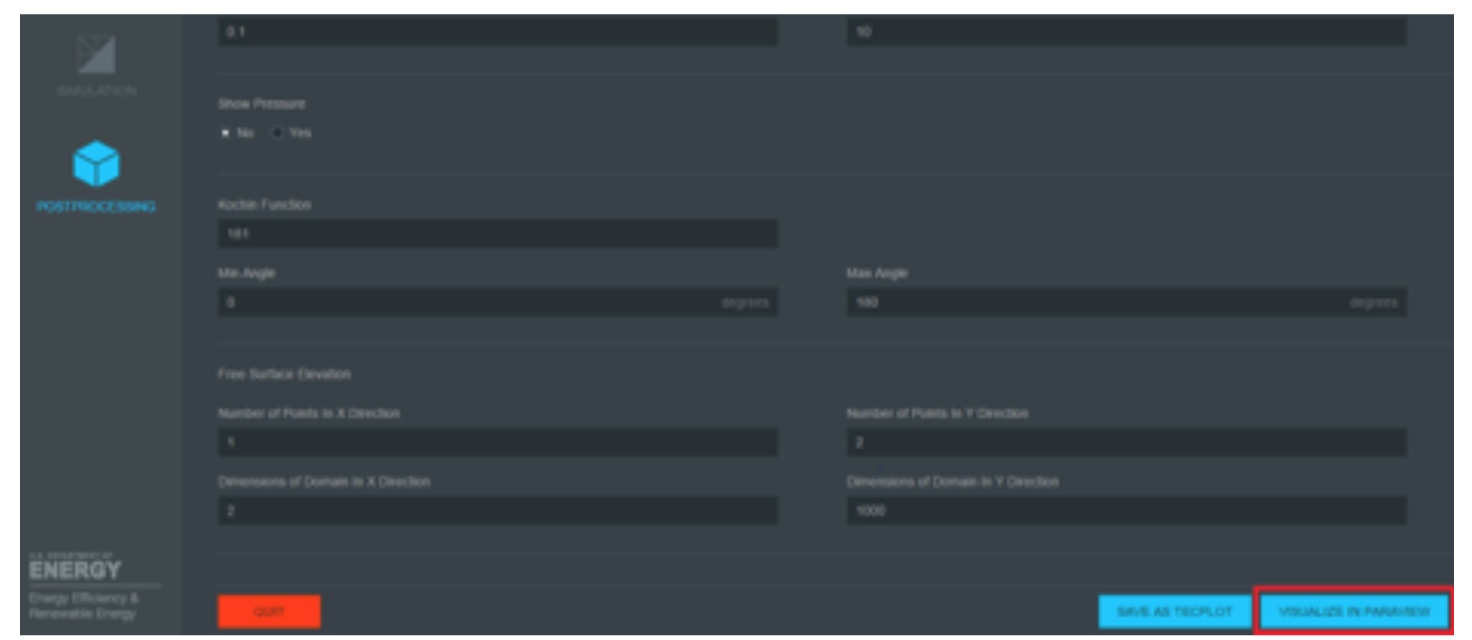
\includegraphics[scale=0.4]{img/37}
	%\captionof{figure}{Transfer from R1 to R2 whenK1=1}
\end{minipage}
\vspace{\belowdisplayskip}

ParaView will start and you will find the resulting forces on the left side:


\vspace{\abovedisplayskip}
\begin{minipage}{\linewidth}
	\centering
	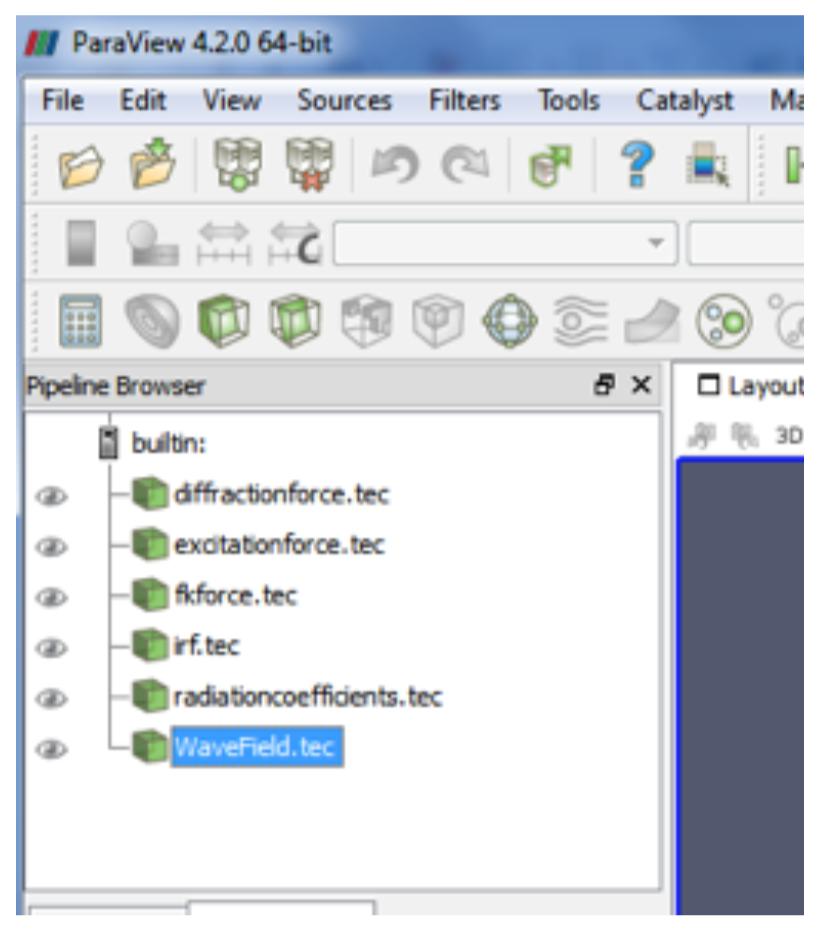
\includegraphics[scale=0.5]{img/38}
	%\captionof{figure}{Transfer from R1 to R2 whenK1=1}
\end{minipage}
\vspace{\belowdisplayskip}

\subsection{Getting help}

You can click on the Help icons displayed on each page:

\vspace{\abovedisplayskip}
\begin{minipage}{\linewidth}
	\centering
	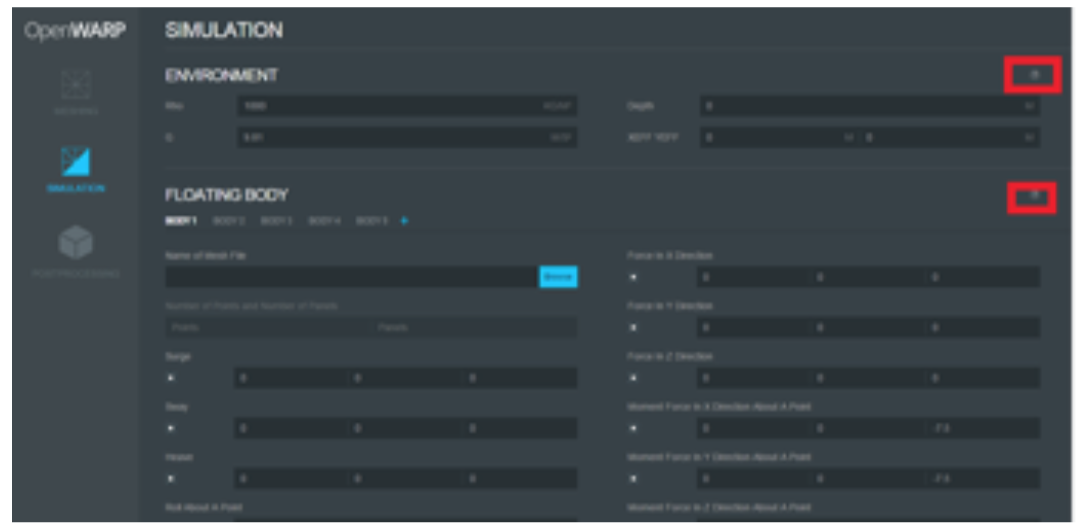
\includegraphics[scale=0.4]{img/39}
	%\captionof{figure}{Transfer from R1 to R2 whenK1=1}
\end{minipage}
\vspace{\belowdisplayskip}

\subsection{Logging Support}

To configure the logging click on the CONFIGURATION screen as shown below:

\vspace{\abovedisplayskip}
\begin{minipage}{\linewidth}
	\centering
	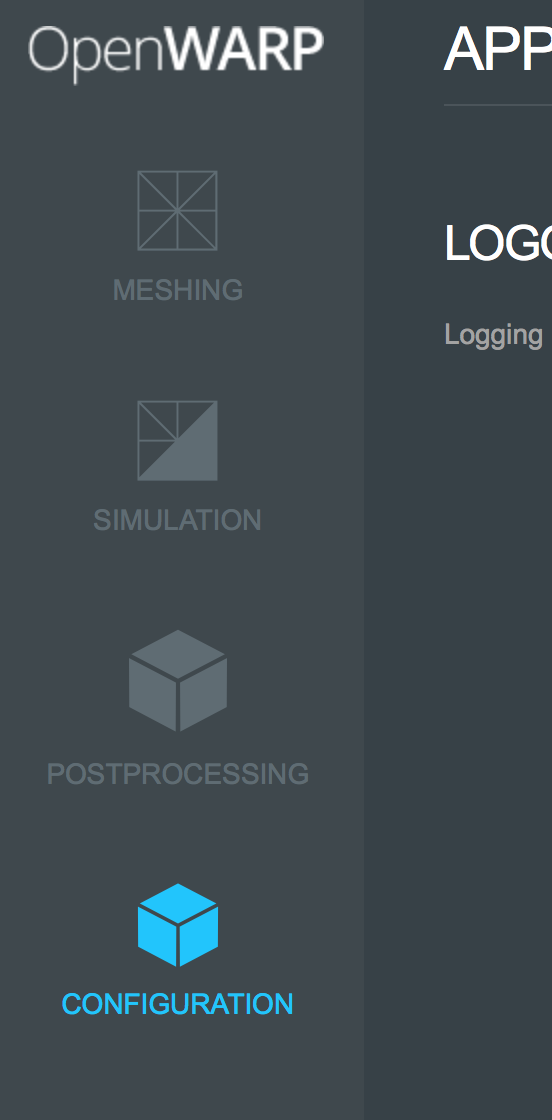
\includegraphics[scale=0.5]{img/39-2}
	%\captionof{figure}{Transfer from R1 to R2 whenK1=1}
\end{minipage}
\vspace{\belowdisplayskip}

After setting the configuration as your wish, you should click on
"APPLY CHANGES" to make sure your changes are taken into account.

\vspace{\abovedisplayskip}
\begin{minipage}{\linewidth}
	\centering
	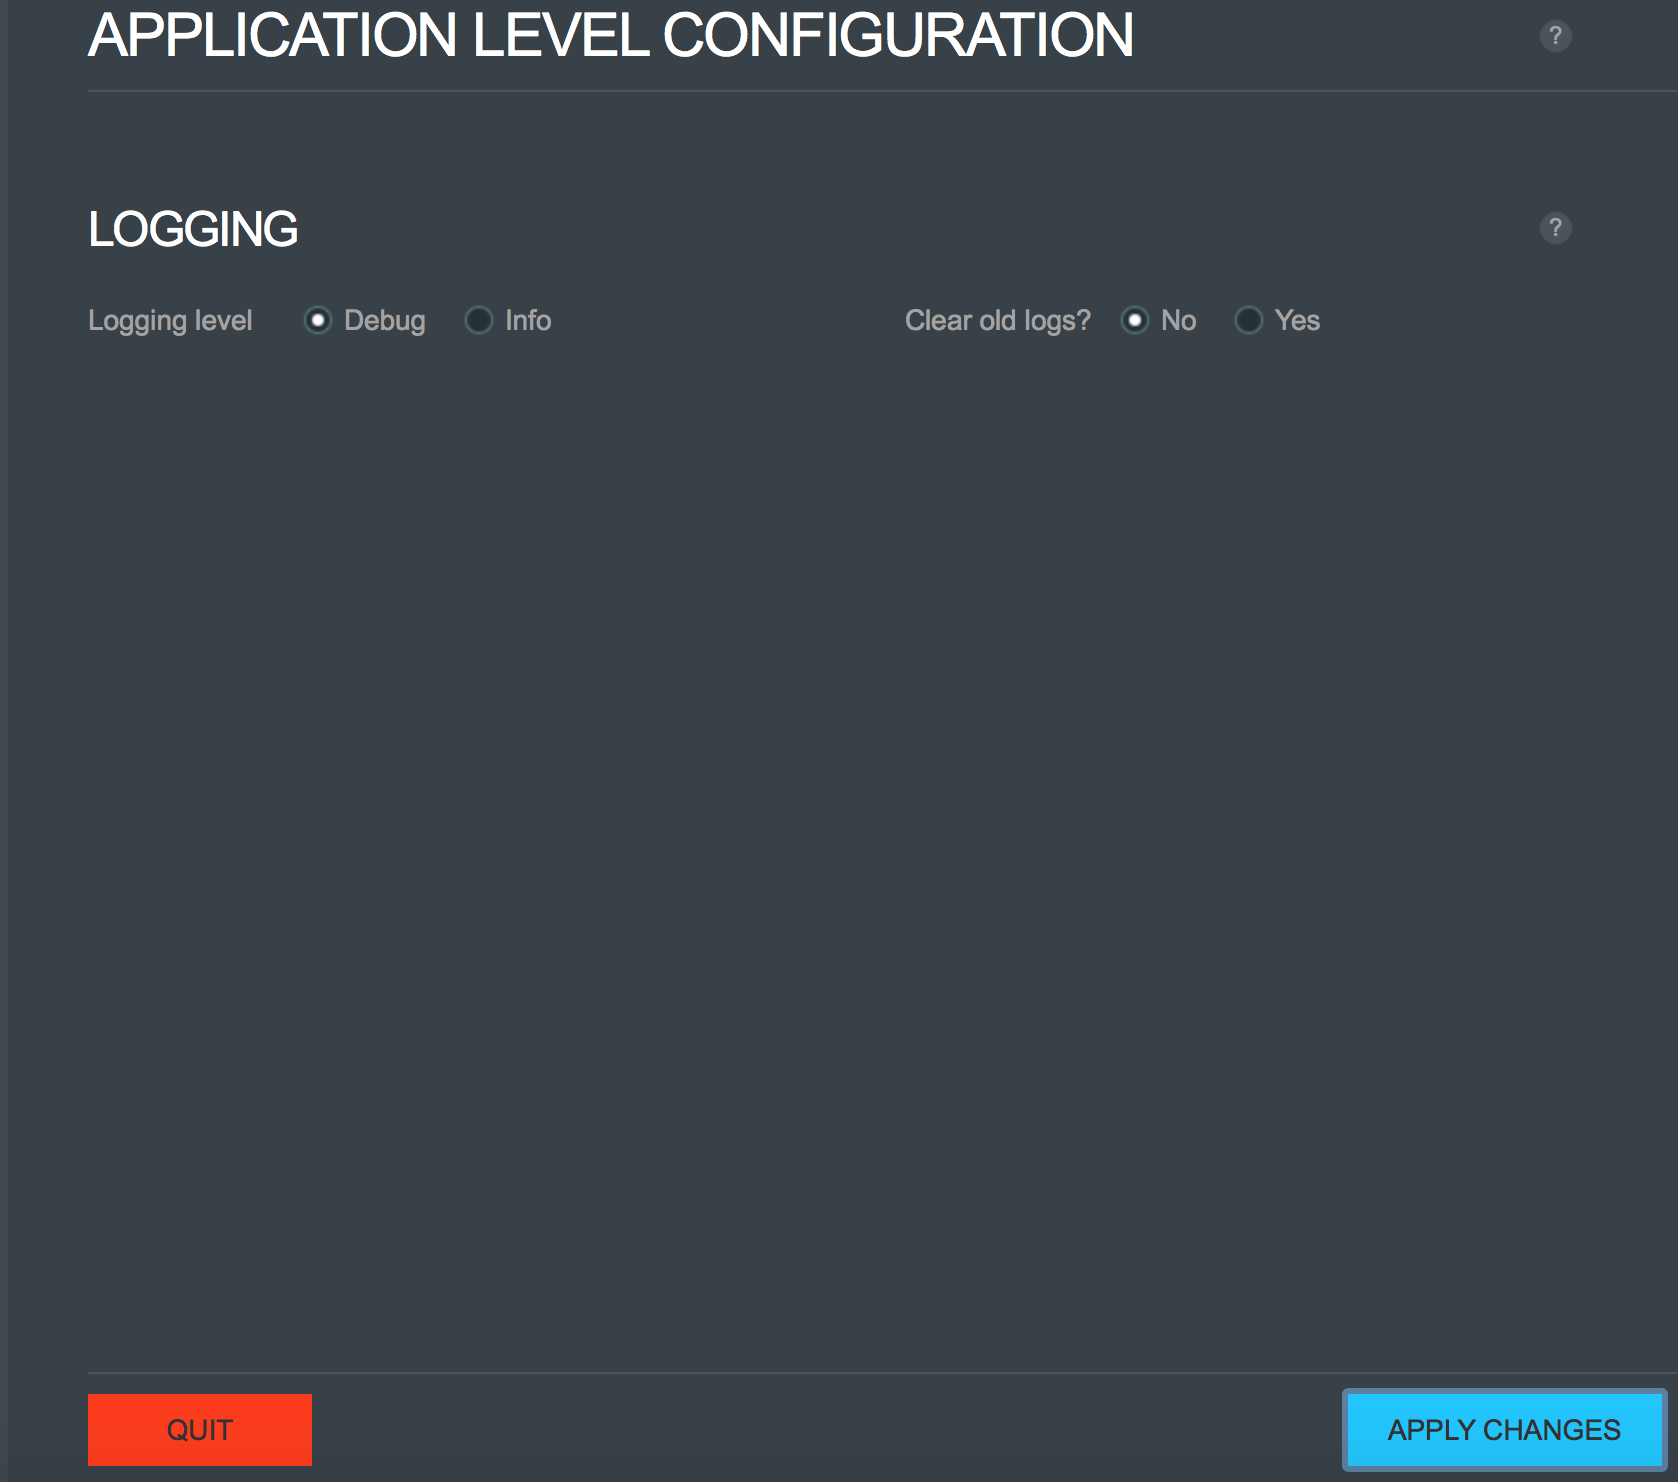
\includegraphics[scale=0.5]{img/40}
	%\captionof{figure}{Transfer from R1 to R2 whenK1=1}
\end{minipage}
\vspace{\belowdisplayskip}

Once done, you will get a status of the change request as well as the location where the logs are saved.

\vspace{\abovedisplayskip}
\begin{minipage}{\linewidth}
	\centering
	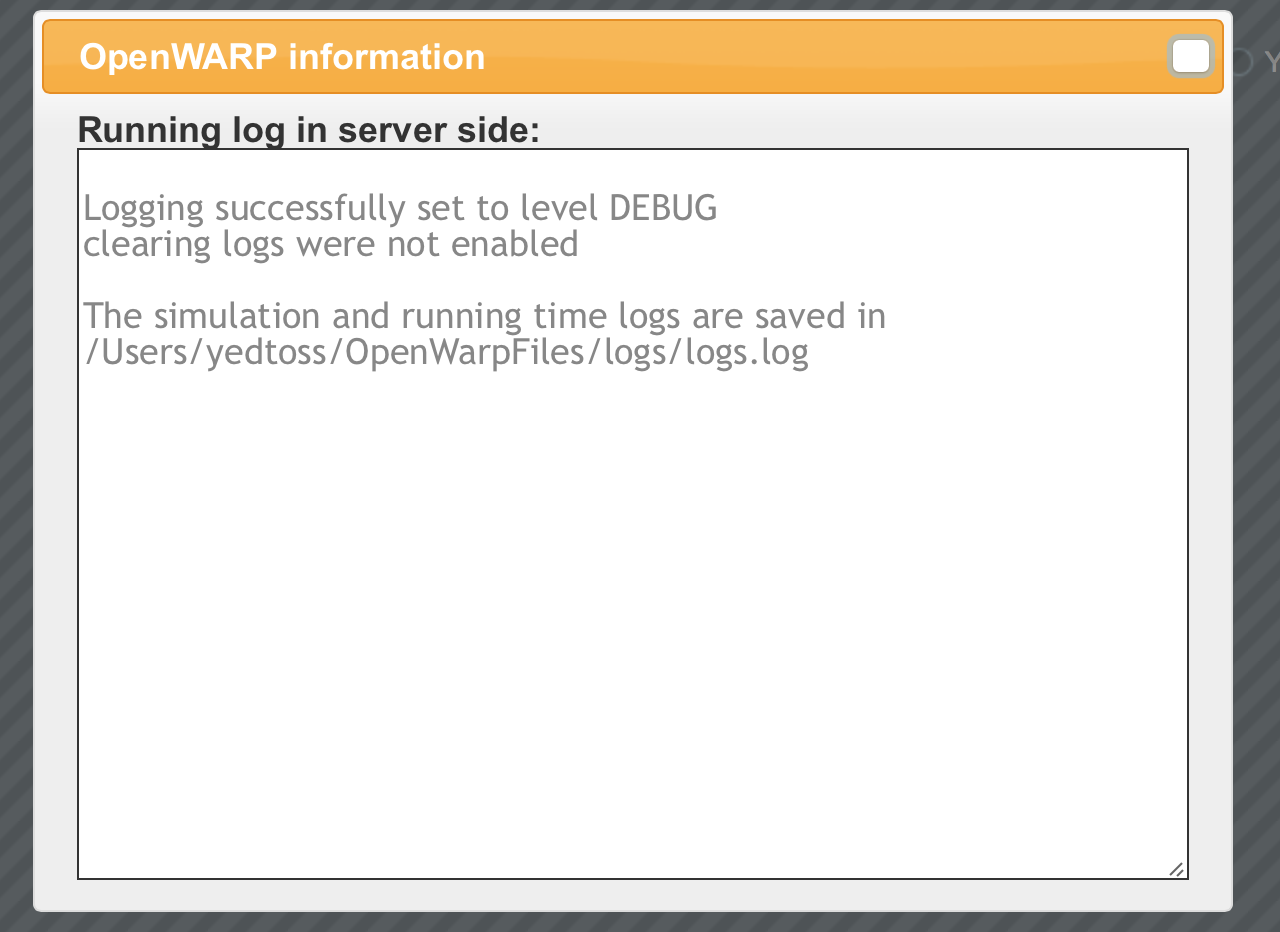
\includegraphics[scale=0.5]{img/41}
	%\captionof{figure}{Transfer from R1 to R2 whenK1=1}
\end{minipage}
\vspace{\belowdisplayskip}

\section{Python CLI}
In order to run the application through the command line instead of through the GUI, the application also provides a command line interface that is suitable to be used when running batch jobs.

You can find this in the source/openwarpgui/ directory. The filename is openwarp_cli.py

Before being able to run the CLI, you should setup your environment library to contain the Nemoh Fortran library directory.

Note that the setup of the environment variables was done in the one-click installers in the script run.sh run.command and run.bat respectively for linux, OS X and Windows. Those files are available from the installers. And they run directly the GUI after setting up the environment variables.

We suggest that when the one-click installers are rebuilt, they include such facility scripts for running the CLI too. In the meantime, one can source the existing script to run the GUI and then quit them using Control + C before starting the CLI. To source the script use:
source run.sh ; source run.command ; call run.bat respectively for Linux, OS X and Windows

To use the openwork cli, simply run: python openwarp_cli.py configuration1 ... where configuration* is the path to the configuration file or a JSON string The configuration fields follow an intuitive name easy to identify and comparable to the one in the GUI screens.

There is a "phase field". Set it to "MESHING" to only do the meshing step.
Set it to "POSTPROCESSING" to only do the postprocessing step, set it to "SIMULATION" to only do the simulation step. When set to None or empty array, all the steps are automatically done.

You can define multiple simulations in the configurations by specifying a different ID for each one. To avoid repeating the same settings, you can specify common settings in the simulations with id "default". Similarly, within in each simulation, you can defined multiple bodies with different ID for each one. Common bodies settings can be defined with the body with id "default".

You can specify which simulations to run by configuring the field: "simulations_to_run". It should an array of simulations ID. Note that the "default" ID is reserved and is not run. It is only used to provide default parameters. If you set "simulations_to_run" to None or empty array, all
simulations are run. You can set the "verbosity" setting to 0 to disable most logging output from the terminal screen. Note that all logs would still be added to the logging file. Set the "verbosity" to any integer higher than 0 to show all output also on screen.

\subsection{CLI Verification}
For all test cases cross checked that at least the input values inside the db.hdf5 match the configuration given in the JSON file. The db.hdf5 file will be located inside the tested simulation directory. All simulation directories are sub-directory of source/openwarpgui/test_files/cli_results
Following have been executed in the OSX environment but it should be possible to replicate in others too.

\begin{enumerate}
\item Basic Testing
Run python openwarp_cli.py test_files/configs/cylinder.json
This test is just to make sure that all the configurations are working correctly

\item shell_step.json
This test is to make sure that the command line will automatically generate a mesh file in the dat format without the user needing to specify it. Indeed, Nemoh only support DAT_FILE. And in the GUI, one can use the MESHING screen to convert a file in (shell, stl, igs) to dat file before giving
it as input in the SIMULATION SCREEN. The command line interface simplify this and make do this conversion when needed.
After a successful run of this test you should see a directory meshing inside the simulation directory with the dat created and used.

\item multiple_sim_same_mesh.json
This is to test that we can run multiple different simulations with the same mesh file. 
Make sure the simulations defined here are generated

\item same_conf_diff_geometry.json
This is to test that we can run multiple different simulations with the same configurations on different geometry.

\item flapsingle_igs.json
This is to test the flapsingle geometry.
This will take an awfully lot of time (More that 10h) to complete and require a lot of memory.

\item Error Message
When the configuration is invalid or the command misused an appropriate error message is shown

\end{enumerate}

\section{Automated TestScript}

Under source/automated test folder, there are  11 test cases implemented. Refer theory documentation for details on each Test.

\subsection{Repository}
\begin{itemize}
\item source/installer.sh - Install all the pre-requisite software required
\item source/testscript.sh - Script to trigger all the test from test1 to test6
\item source/testscript2.sh - Script to trigger all the test from test7 to test11
\item source/automated test/ - Directory contains workspace  for each tests. All the output results gets created here.
\item source/automated_test.log - log file for testscript
\item source/automated_test2.log - log file for testscrpt2
\item doc/deployment_guide.pdf - Deployment guide to start OpenWarp in general.
\end{itemize}

\subsection{Dependencies}
All the prerequisite software and there installations are listed above under dependencies.Following modules are dependent to tests:
\begin{itemize}
\item 1.	openwarp_cli.py - All test, except test1 uses openwarp_cli.py. For details informations, refer Python CLI section in this doc or under Contest_Output/PythonCLI. Testscript.sh source run.sh to set the environment variables and dependencies. Testscript2.sh also set environment variables to succesfully run openwarp_cli.py
\item 2.	Bemio - Test are written in such a way that, it has merged only the subpart of Bemio here and there according to individual test requirement.
\item 3.	H5DIFF- H5DIFF utility comes with HDF5-TOOLS set. To install in ubuntu ,sudo apt-get install hdf5-tools command can be used. although it covered in installer.sh
\item 4.	Wamit testruns -  Wamit testruns directory to make use of Wamit's test and its output to compare with OpenWarp output.
\end{itemize}

Following sections briefly describe each test case:
\subsection{Test 1: Converting GDF to OpenWarp Format}
\subsubsection{Objective of Test case}
To convert Wamit' GDF file to DAT file to make it compatible with OpenWarp.
\subsubsection{Steps to execute the test}
Run testscript.sh
\subsubsection{Output}
All the subsequent GDF files of Wamit are convert to .DAT format under automated_test/testruns/openwarp/**.dat
Outputlog: automated_test.log

\subsection{Test 2: Wamit Test Input and Output} 
\subsubsection{Objective of Test case}
To convert Wamit's output in H5 format.
To run Wamit's GDF files(by convert to DAT from test 1)
To compare Wamit's Ouput to new OpenWarp output
\subsubsection{Steps to execute the test}
Run testscript.sh, it will automatically run Test2 after executing test1 cases.
\subsubsection{Output and Comparison}
.H5 files under testruns/ db.hdf5 
db.hdf5 files under automated_test/testruns/openwarp/openwarpH5
test*.log under Test2 (it contains comparison against all 11 types of outputs). The comparison is done objects by objects using H5DIFF tool.
Outputlog: automated_test.log


\subsection{Test 3: Testing HigherOrder Implementation in OpenWarp}
\subsubsection{Objective of Test case}
To test difference in output for B_SPLINE Order under higher order implementation.
\subsubsection{Steps to execute the test}
Run testscript.sh, it will automatically run Test3 to create an output by using Wamit's test11 to test25
\subsubsection{Output and Comparison}
testlogs under test3.log
Outputlog: automated_test.log

\subsection{Test 4: Testing the Dipoles/Thin Panels implementation in OpenWarp}
\subsubsection{Objective of Test case}
To test differences in output while dipoles and thin panels implementation
\subsubsection{Steps to execute the test}
Run testscript.sh
\subsubsection{Output and Comparison}
testlogs under test4.log
Outputlog: automated_test.log

\subsection{Test 5: Testing Irregular Frequency Removal in OpenWarp}
\subsubsection{Objective of Test case}
To test difference in values of objects with irregular frequency in higher as well as lower order implementation
\subsubsection{Steps to execute the test}
Run testscript.sh
\subsubsection{Output and Comparison}
testlogs under test5.log
Outputlog: automated_test.log

\subsection{Test 6: Testing Mean Drift Forces and Yaw moment Implementation in OpenWarp}
\subsubsection{Objective of Test case}
To test difference in values in horizontal drift forces and mean yaw moment by momentum integration.
\subsubsection{Steps to execute the test}
Run testscript.sh
\subsubsection{Output and Comparison}
testlogs under automated_Test/Test6
Outputlog: automated_test.log

\subsection{Test 7: Computation of the Green Function using ordinary differential equation in OpenWarp}
\subsubsection{Objective of Test case}
To determine the difference in values of Green Function when ODE method is used to calculate influence coefficients.
\subsubsection{Steps to execute the test}
Run testscript2.sh
\subsubsection{Output and Comparison}
testlogs under automated_test/Test7
Outputlog: automated_test2.log

\subsection{Test 8: Testing Green Function Tabulation Implementation}
\subsubsection{Objective of Test case}
To see the difference in tabulated data makes under Green function
\subsubsection{Steps to execute the test}
Run testscript2.sh
\subsubsection{Output and Comparison}
testlogs under automated_test/Test8
Outputlog: automated_test2.log

\subsection{Test 9: 2Bodies}
\subsubsection{Objective of Test case}
To execute simulation and postprocessing for common values and multiple simulation case.
\subsubsection{Steps to execute the test}
Run testscript2.sh. automated_test/Test9/2bodies.json has the updated values from Nemoh.cal
\subsubsection{Output and Comparison}
testlogs under automated_test/Test9
Outputlog: automated_test2.log

\subsection{Test 10: Cylinder}
\subsubsection{Objective of Test case}
To execute simulation and postprocessing for cylinderical geometry.
\subsubsection{Steps to execute the test}
Run testscript2.sh, automated_test/Test10/cylinder.json has the updated values from Nemoh.cal
\subsubsection{Output and Comparison}
testlogs under automated_test/Test10
Outputlog: automated_test2.log

\subsection{Test 11: NonSymmetrical}
\subsubsection{Objective of Test case}
To execute simulation and postprocessing for NonSymmetrical geomerty
\subsubsection{Steps to execute the test}
Run testscript2.sh, automated_test/Test11/nonsymmetrical.json has the updated values from Nemoh.cal 
\subsubsection{Output and Comparison}
testlogs under automated_test/Test11
Outputlog: automated_test2.log


\section{Steps to update OW from Nemoh 2014 to Nemoh 2016}
When OW was created, we used Nemoh version 2014. At the time of writing this document, the version of Nemoh is 2016. Thus, the following outlines the steps to follow when including the updates carried out in Nemoh 2016 into OpenWarp.

\begin{enumerate}
\item First, look for the new code implemented in Nemoh using mercurial diff tool
\item Next, check if they were implemented in the python package or the Fortran part of OW. Preprocessor and postprocessor code in Nemoh are in python part of OW whereas most of the Solver code is in Fortran part of OW. After this step, one should have identified the file and lines where it is implemented / needs to be implemented in OW.
\item Check if the fixed / new code is relevant to OW. Most of the Solver related code in Nemoh is relevant to OW. Preprocessor and postprocessor code are not always relevant.
\item We also need to keep in mind the new features implemented in OW. For example, OW Fortran solver does not write / save to files and as such code changes should be ignored in such aspects. Also, keep in mind Fortran code in OW used Fortran 2003 and uses standard functions instead of vendor specific functions as much as possible. As a result, before changing a function, make sure that OW was not using an equivalent standard function. OW also replaced some functions with their recommended 2003 equivalent. Watch out for these and ignore them. Finally, OW avoids the use of GOTO statement and such changes can also be ignored.
\item As a general rule of thumb, the only fixes to add are the ones that change the computation, not the ones that are doing the same computation using a different approach / style of coding.
\item After all the assessment has been carried out and the changes to carry out have been conclusively determined, apply the changes.
\end{enumerate}


\section{Practical Example}

We are going to use the FlapSingle example available in \ROOT/test_files where \ROOT is the top-level directory of the OpenWarp package. It is also available in \INSTALLDIR/OpenWarp/test_files
First, we will generate the mesh of the body. Next, we will run the simulation. Finally, we will generate the TEC files and visualize them.

\subsection{Mesh Generation}
Go to the Meshing page, click on Browse, and choose \ROOT/test_files/mesh/FlapSingle.stl where \ROOT is the top-level directory of the OpenWarp package and Execute the meshing:

\vspace{\abovedisplayskip}
\begin{minipage}{\linewidth}
	\centering
	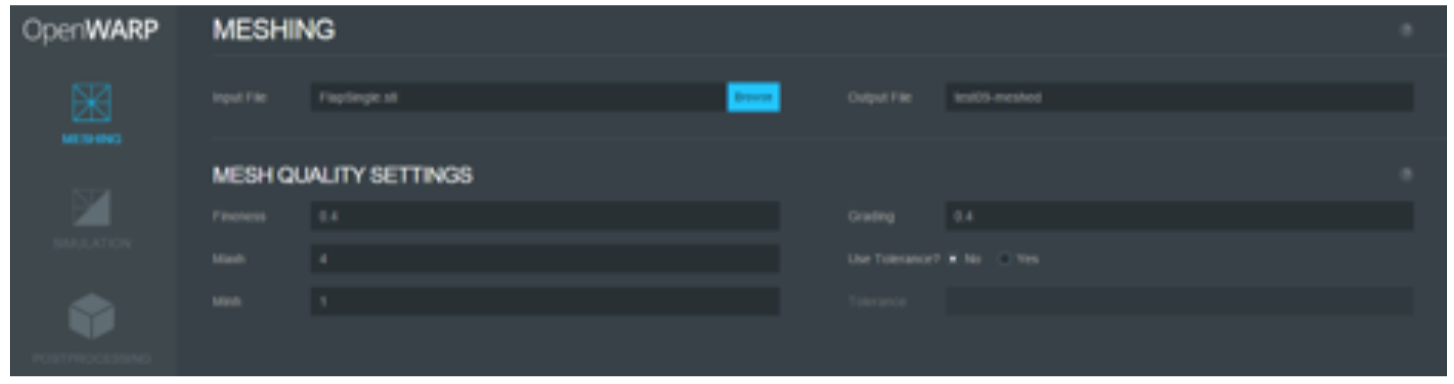
\includegraphics[scale=0.5]{img/42}
	%\captionof{figure}{Transfer from R1 to R2 whenK1=1}
\end{minipage}
\vspace{\belowdisplayskip}



%\begin{minipage}{\linewidth}
%	\centering
%	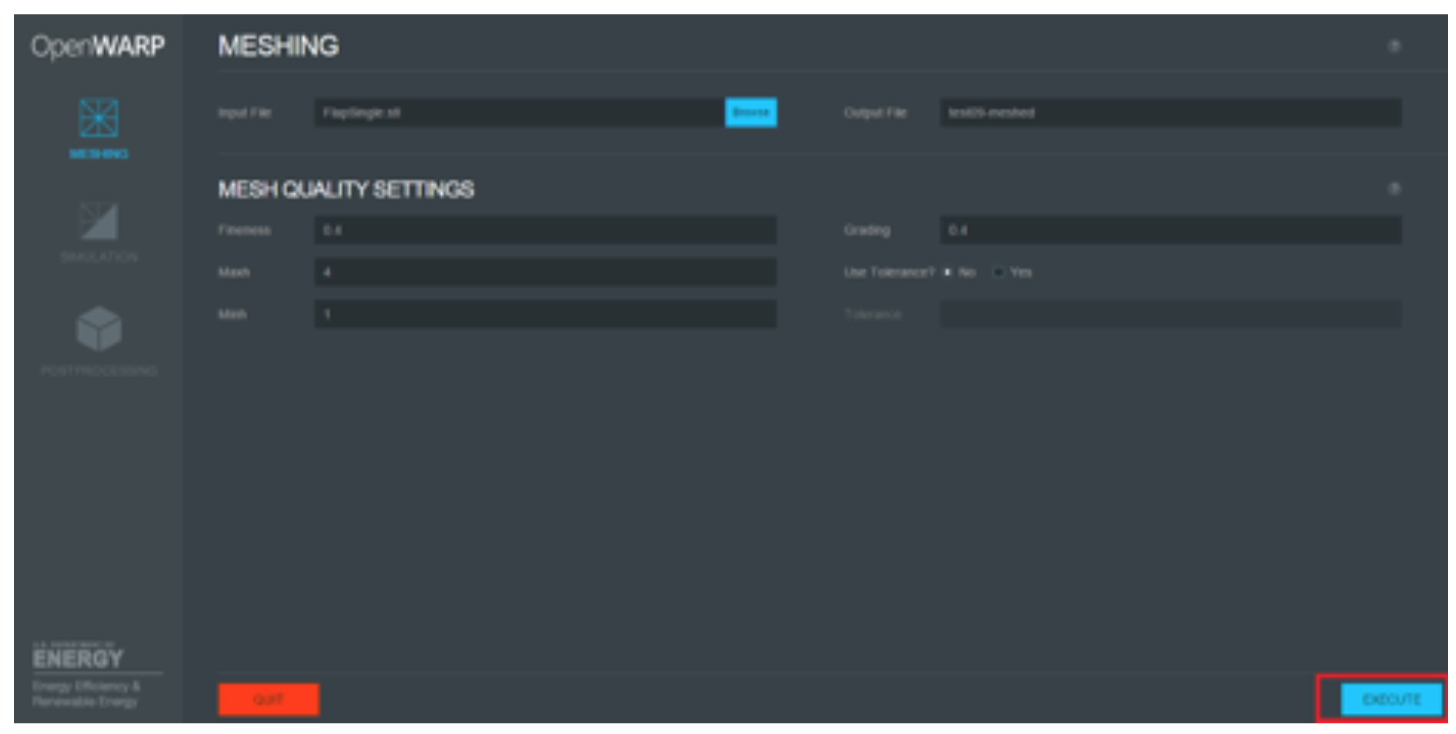
\includegraphics[scale=0.7]{img/43}
%	%\captionof{figure}{Transfer from R1 to R2 whenK1=1}
%\end{minipage}

You will see the results shown like this :

\vspace{\abovedisplayskip}
\begin{minipage}{\linewidth}
	\centering
	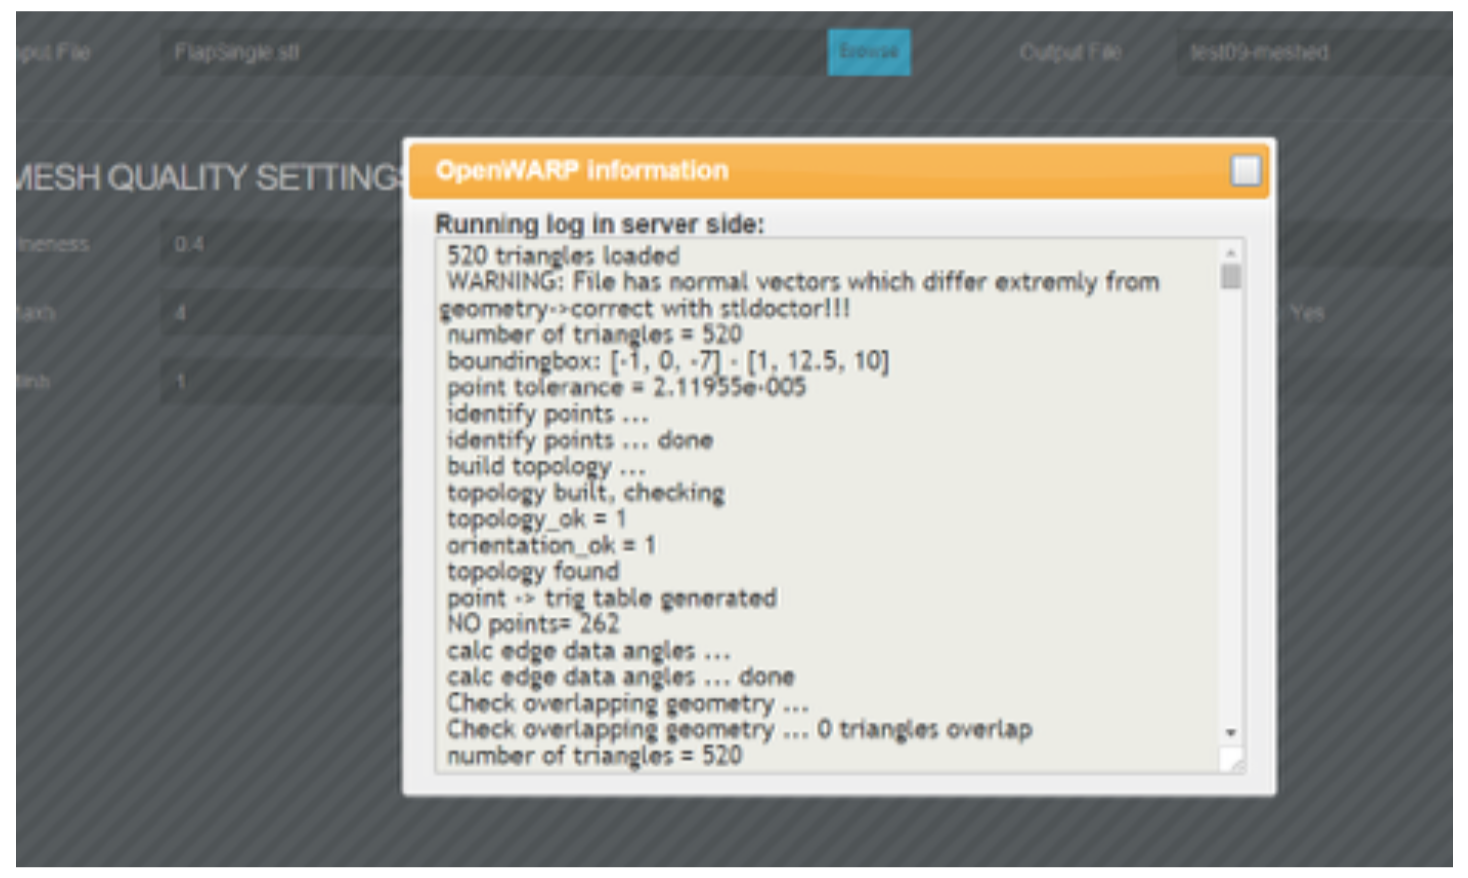
\includegraphics[scale=0.5]{img/45}
	%\captionof{figure}{Transfer from R1 to R2 whenK1=1}
\end{minipage}
\vspace{\belowdisplayskip}



%\begin{minipage}{\linewidth}
%	\centering
%	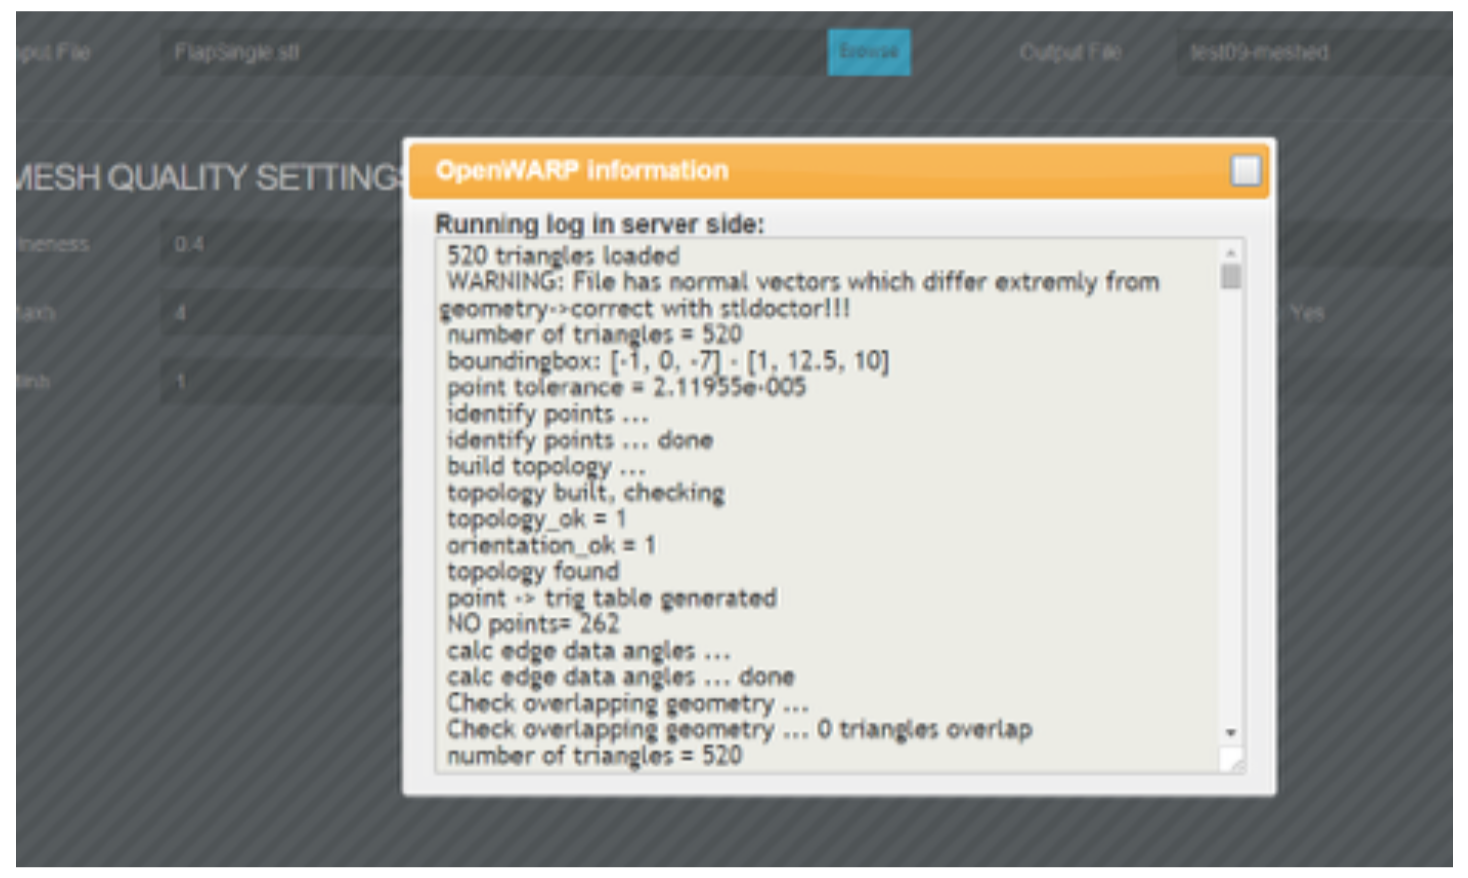
\includegraphics[scale=0.7]{img/45}
%	%\captionof{figure}{Transfer from R1 to R2 whenK1=1}
%\end{minipage}


Click the button in the corner of the popup to close it:

\vspace{\abovedisplayskip}
\begin{minipage}{\linewidth}
	\centering
	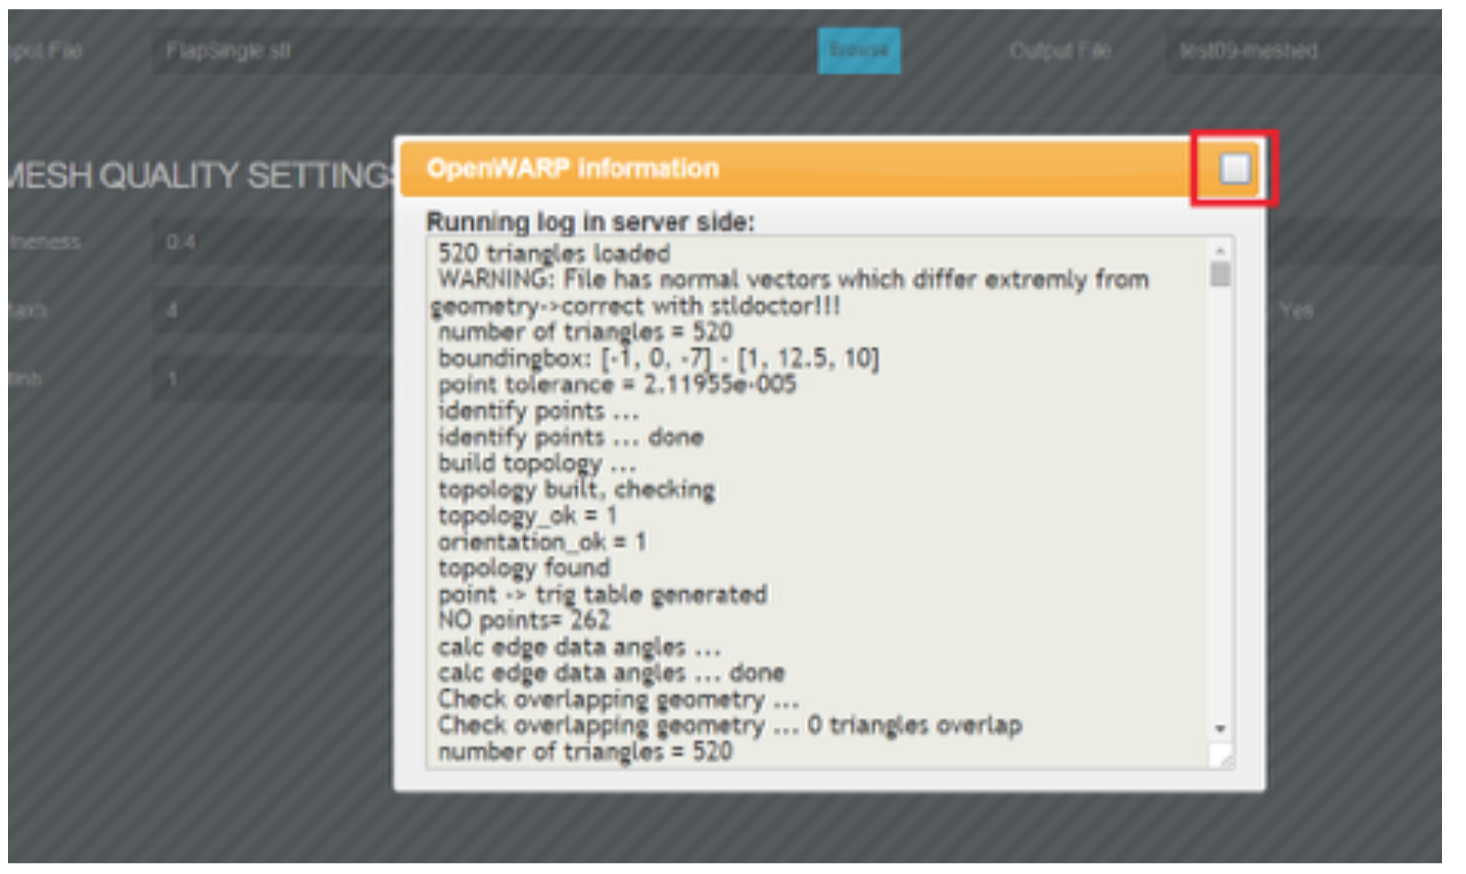
\includegraphics[scale=0.5]{img/46}
	%\captionof{figure}{Transfer from R1 to R2 whenK1=1}
\end{minipage}
\vspace{\belowdisplayskip}

\subsection{Run the simulation}

Go to the simulation page and click on Browse to load the generated mesh file.
The generated mesh file is inside the \$HOME/OpenWarpFiles/user{\_}data/meshing_TIMESTAMP_HASH where
\$HOME is your home directory. Go to the directory with the latest timestamp.

\vspace{\abovedisplayskip}
\begin{minipage}{\linewidth}
	\centering
	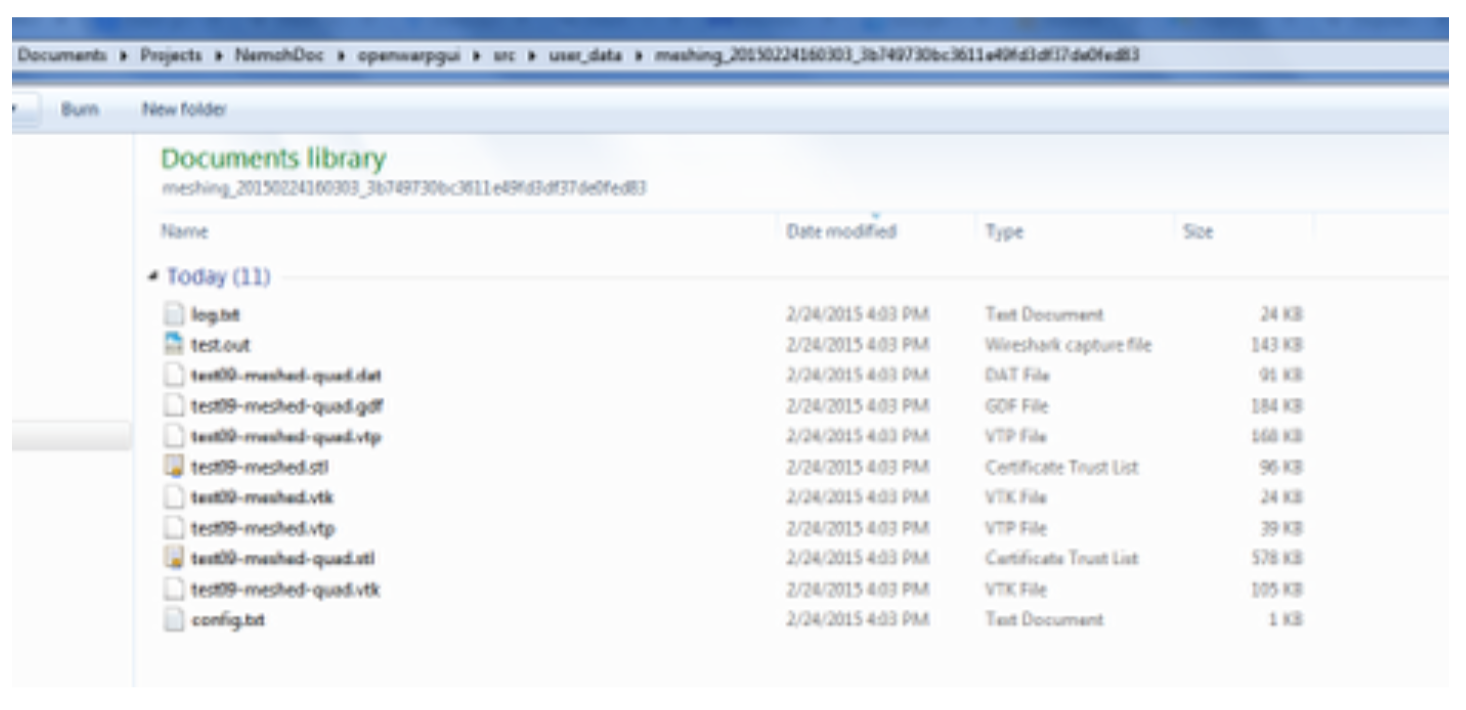
\includegraphics[scale=0.5]{img/47}
	%\captionof{figure}{Transfer from R1 to R2 whenK1=1}
\end{minipage}
\vspace{\belowdisplayskip}

Look for a .dat file. It is named flap-meshed-quad.dat in our case.

\vspace{\abovedisplayskip}
\begin{minipage}{\linewidth}
	\centering
	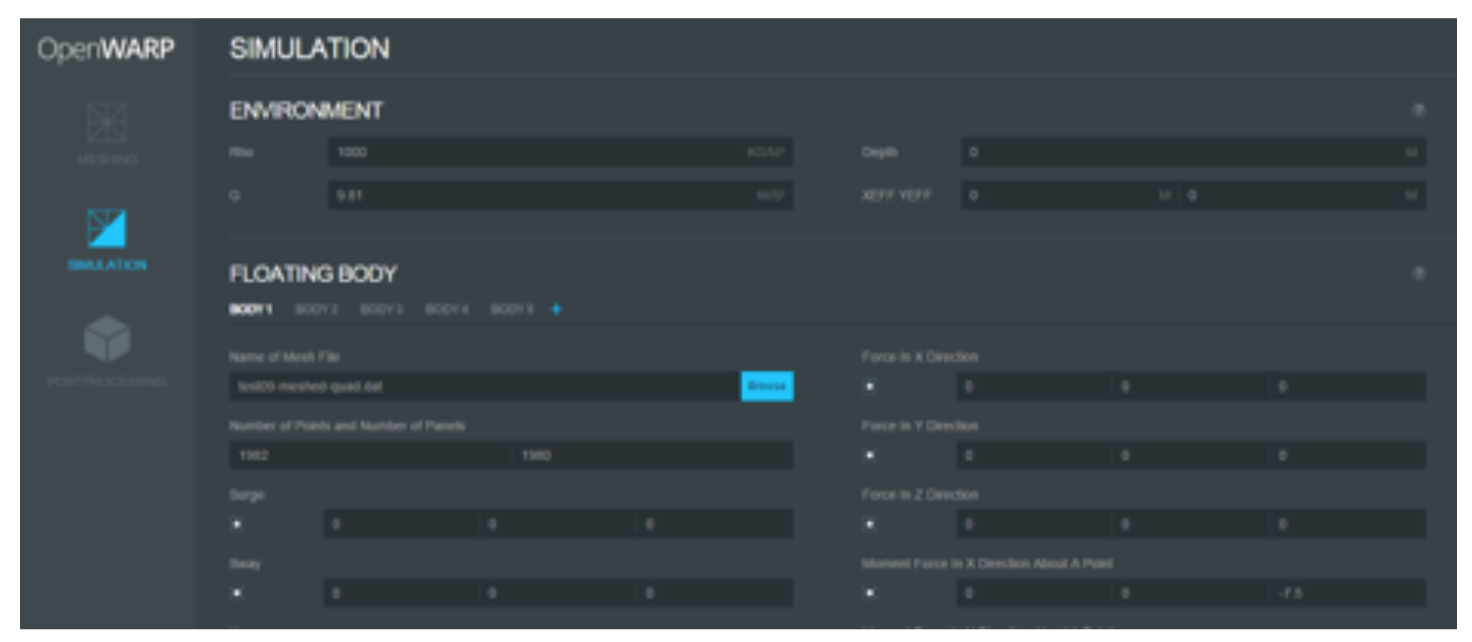
\includegraphics[scale=0.5]{img/48}
	%\captionof{figure}{Transfer from R1 to R2 whenK1=1}
\end{minipage}
\vspace{\belowdisplayskip}

Run the simulation by clicking on "EXECUTE". You should see this:

\vspace{\abovedisplayskip}
\begin{minipage}{\linewidth}
	\centering
	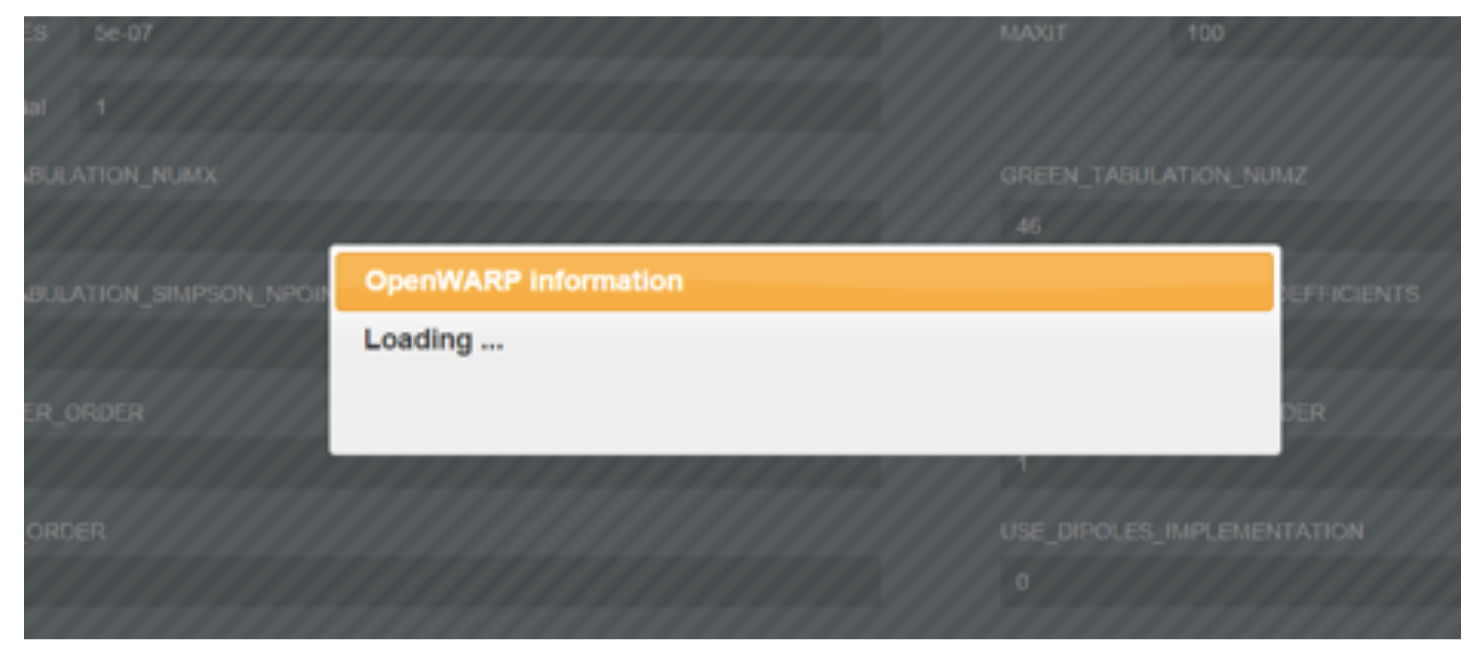
\includegraphics[scale=0.5]{img/49}
	%\captionof{figure}{Transfer from R1 to R2 whenK1=1}
\end{minipage}
\vspace{\belowdisplayskip}

When the simulation is done (You should be patient as it will take a few minutes), the results are summarized in a popup:

\vspace{\abovedisplayskip}
\begin{minipage}{\linewidth}
	\centering
	\includegraphics[scale=0.5]{img/50}
	%\captionof{figure}{Transfer from R1 to R2 whenK1=1}
\end{minipage}
\vspace{\belowdisplayskip}

Close the popup:

\vspace{\abovedisplayskip}
\begin{minipage}{\linewidth}
	\centering
	\includegraphics[scale=0.5]{img/51}
	%\captionof{figure}{Transfer from R1 to R2 whenK1=1}
\end{minipage}
\vspace{\belowdisplayskip}

Inside the directory \$HOME/OpenWarpFiles/user{\_}data/simulation{\_}TIMESTAMP{\_}HASH, you will see the generated simulation results where \$HOME is the home directory of the current user.
Find db.hdf5 inside the directory with the latest timestamp; it contains the results.

\vspace{\abovedisplayskip}
\begin{minipage}{\linewidth}
	\centering
	\includegraphics[scale=0.5]{img/52}
	%\captionof{figure}{Transfer from R1 to R2 whenK1=1}
\end{minipage}
\vspace{\belowdisplayskip}

\subsection{Generate TEC files and run postprocessing}

Open the postprocessing page.
Leave the default values. Generate the TEC files by clicking "Save as TECPLOT". When postprocessing is done, you get a popup:

\vspace{\abovedisplayskip}
\begin{minipage}{\linewidth}
	\centering
	\includegraphics[scale=0.5]{img/53}
	%\captionof{figure}{Transfer from R1 to R2 whenK1=1}
\end{minipage}
\vspace{\belowdisplayskip}

Close it.

\vspace{\abovedisplayskip}
\begin{minipage}{\linewidth}
	\centering
	\includegraphics[scale=0.5]{img/54}
	%\captionof{figure}{Transfer from R1 to R2 whenK1=1}
\end{minipage}
\vspace{\belowdisplayskip}




\subsection{Visualize the generated tec files}

Click on "VISUALIZE IN PARAVIEW".
You will see this while ParaView opens:

\vspace{\abovedisplayskip}
\begin{minipage}{\linewidth}
	\centering
	\includegraphics[scale=0.5]{img/55}
	%\captionof{figure}{Transfer from R1 to R2 whenK1=1}
\end{minipage}
\vspace{\belowdisplayskip}

Once ParaView is open, you will see the generated forces on the left:

\vspace{\abovedisplayskip}
\begin{minipage}{\linewidth}
	\centering
	\includegraphics[scale=0.7]{img/56}
	%\captionof{figure}{Transfer from R1 to R2 whenK1=1}
\end{minipage}
\vspace{\belowdisplayskip}

\end{document}
